 \subsection{Cross-check analysis with independent macros}

There are two independent analysis code used for correlation analyses and the cross check results are documented in this section. The cuts are specified in Table 1 and 2. The first column contains Anthony's analysis, the second contains Austin's cross-check, and the third contains the ratio of the two.
%%%%%%%%%%% LEP1 %%%%%%%%%%%
\begin{figure}[H]
\centering
\subfloat{\label{sfig:a}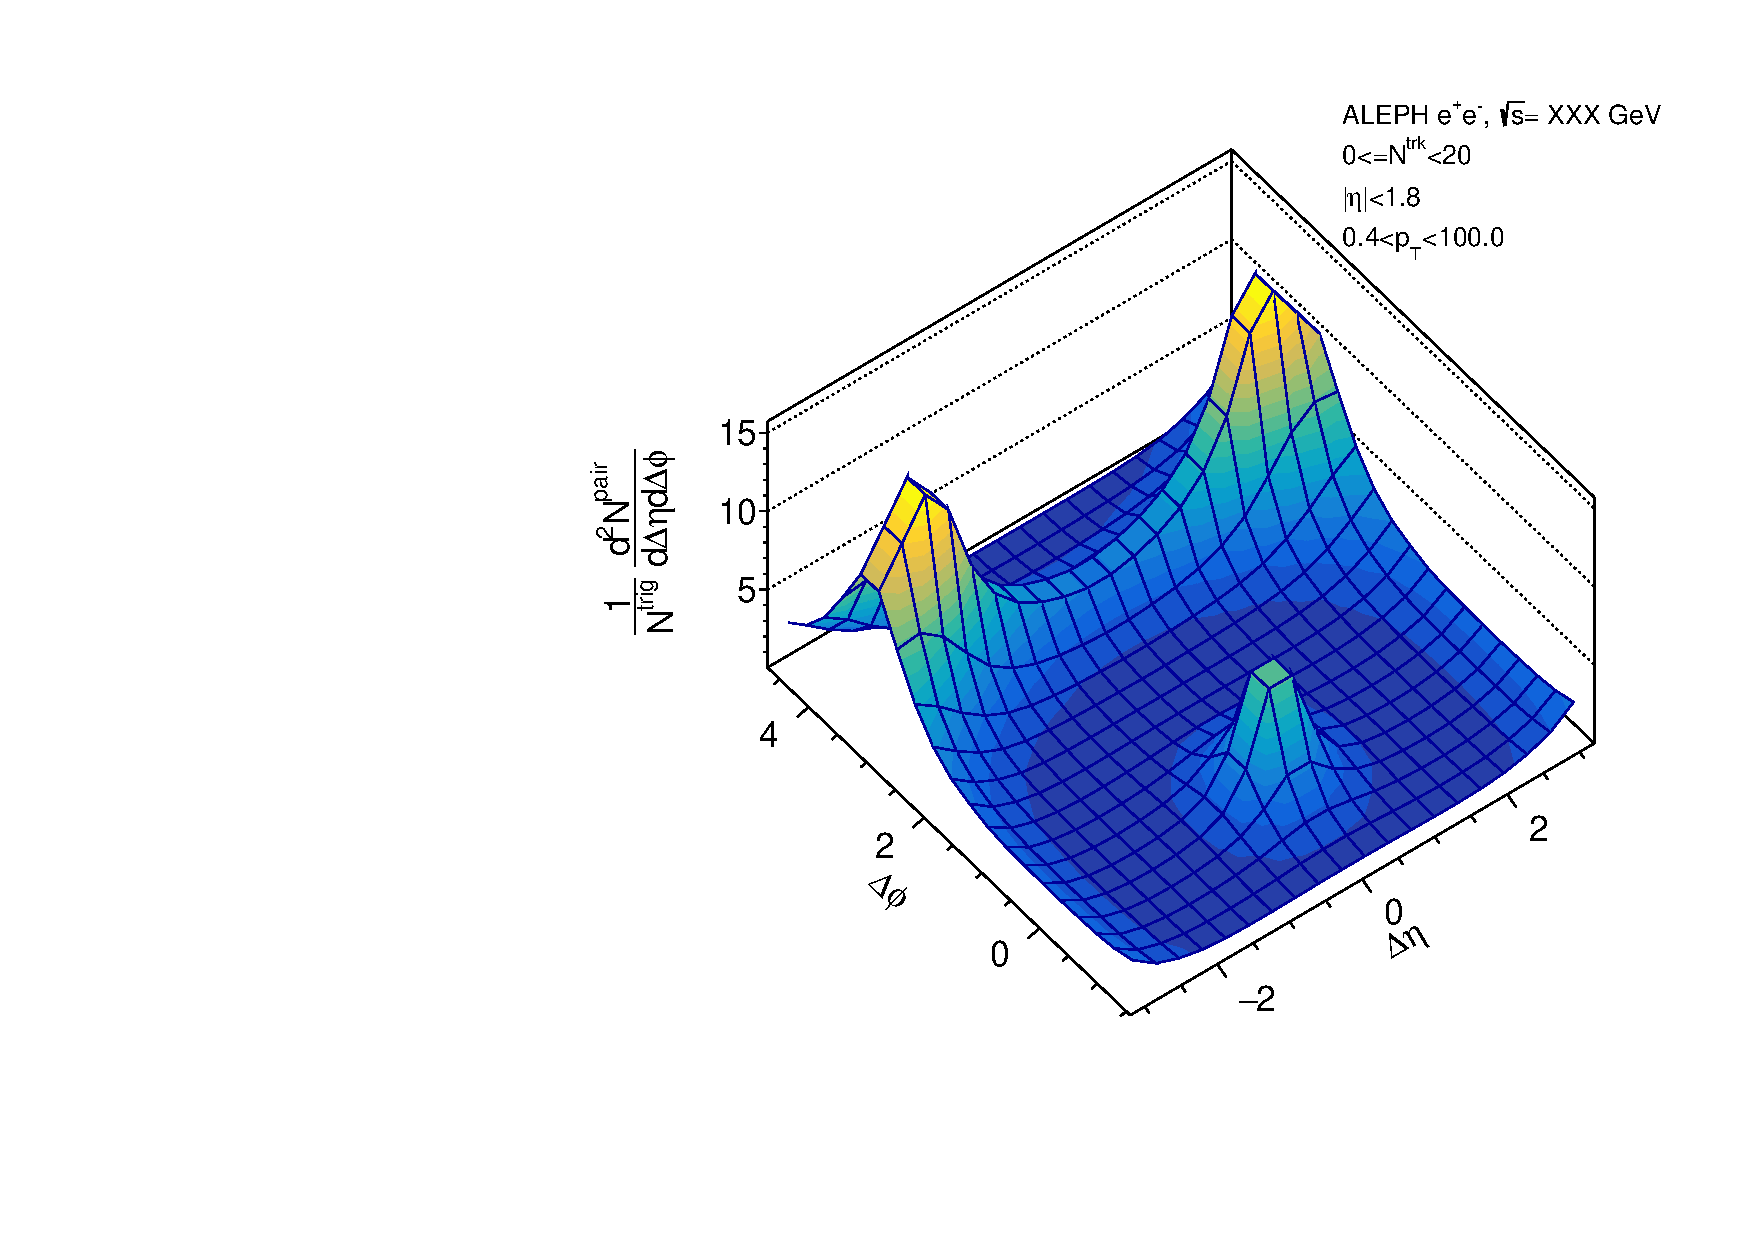
\includegraphics[width=.32\textwidth]{images/TwoParticleCorrelation/CrossCheck/20180126/LEP1_BEAM/LEP1_BEAM_ratio2_0_20.pdf}}\hfill
\subfloat{\label{sfig:b}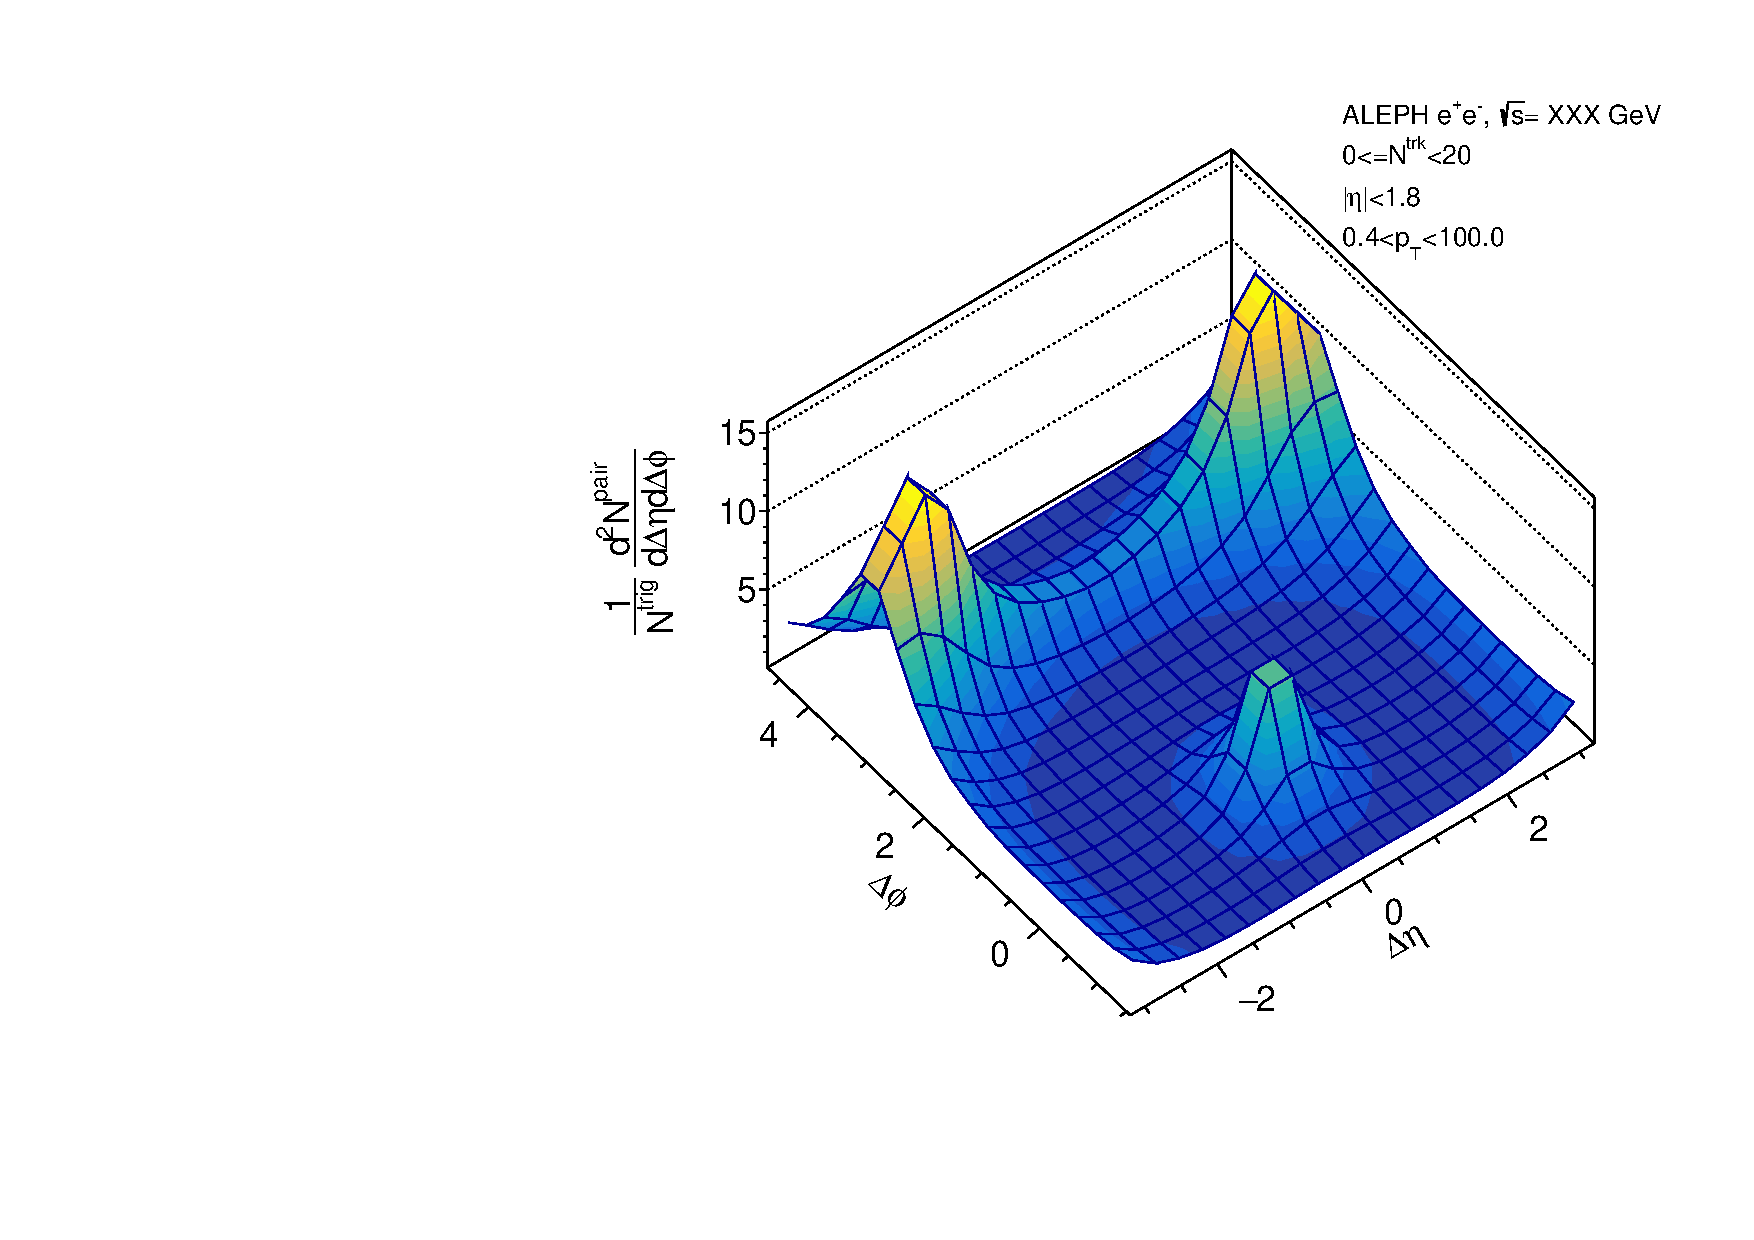
\includegraphics[width=.32\textwidth]{images/TwoParticleCorrelation/CrossCheck/20180126/LEP1_BEAM/LEP1_BEAM_ratio1_0_20.pdf}}\hfill
\subfloat{\label{sfig:c}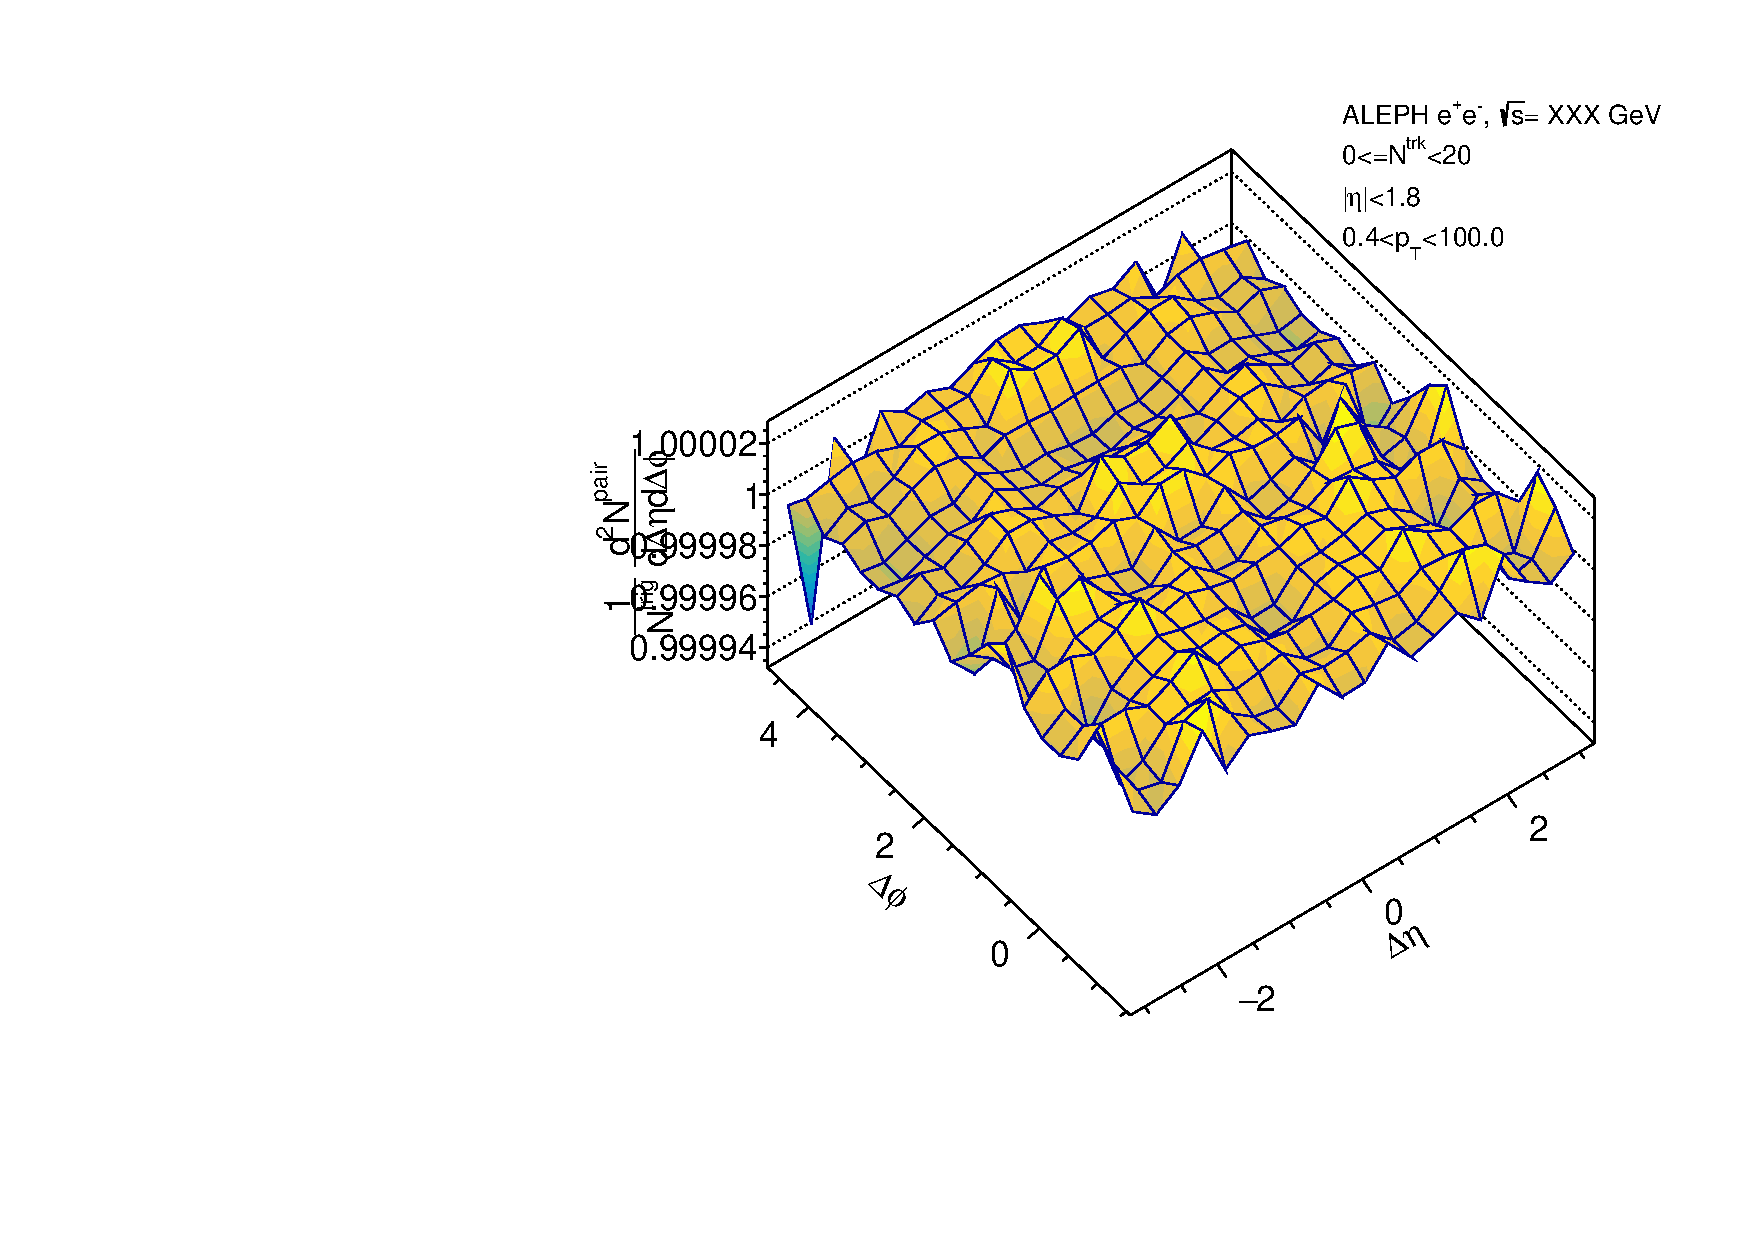
\includegraphics[width=.32\textwidth]{images/TwoParticleCorrelation/CrossCheck/20180126/LEP1_BEAM/LEP1_BEAM_r_ratio_0_20.pdf}}\hfill
\subfloat{\label{sfig:d}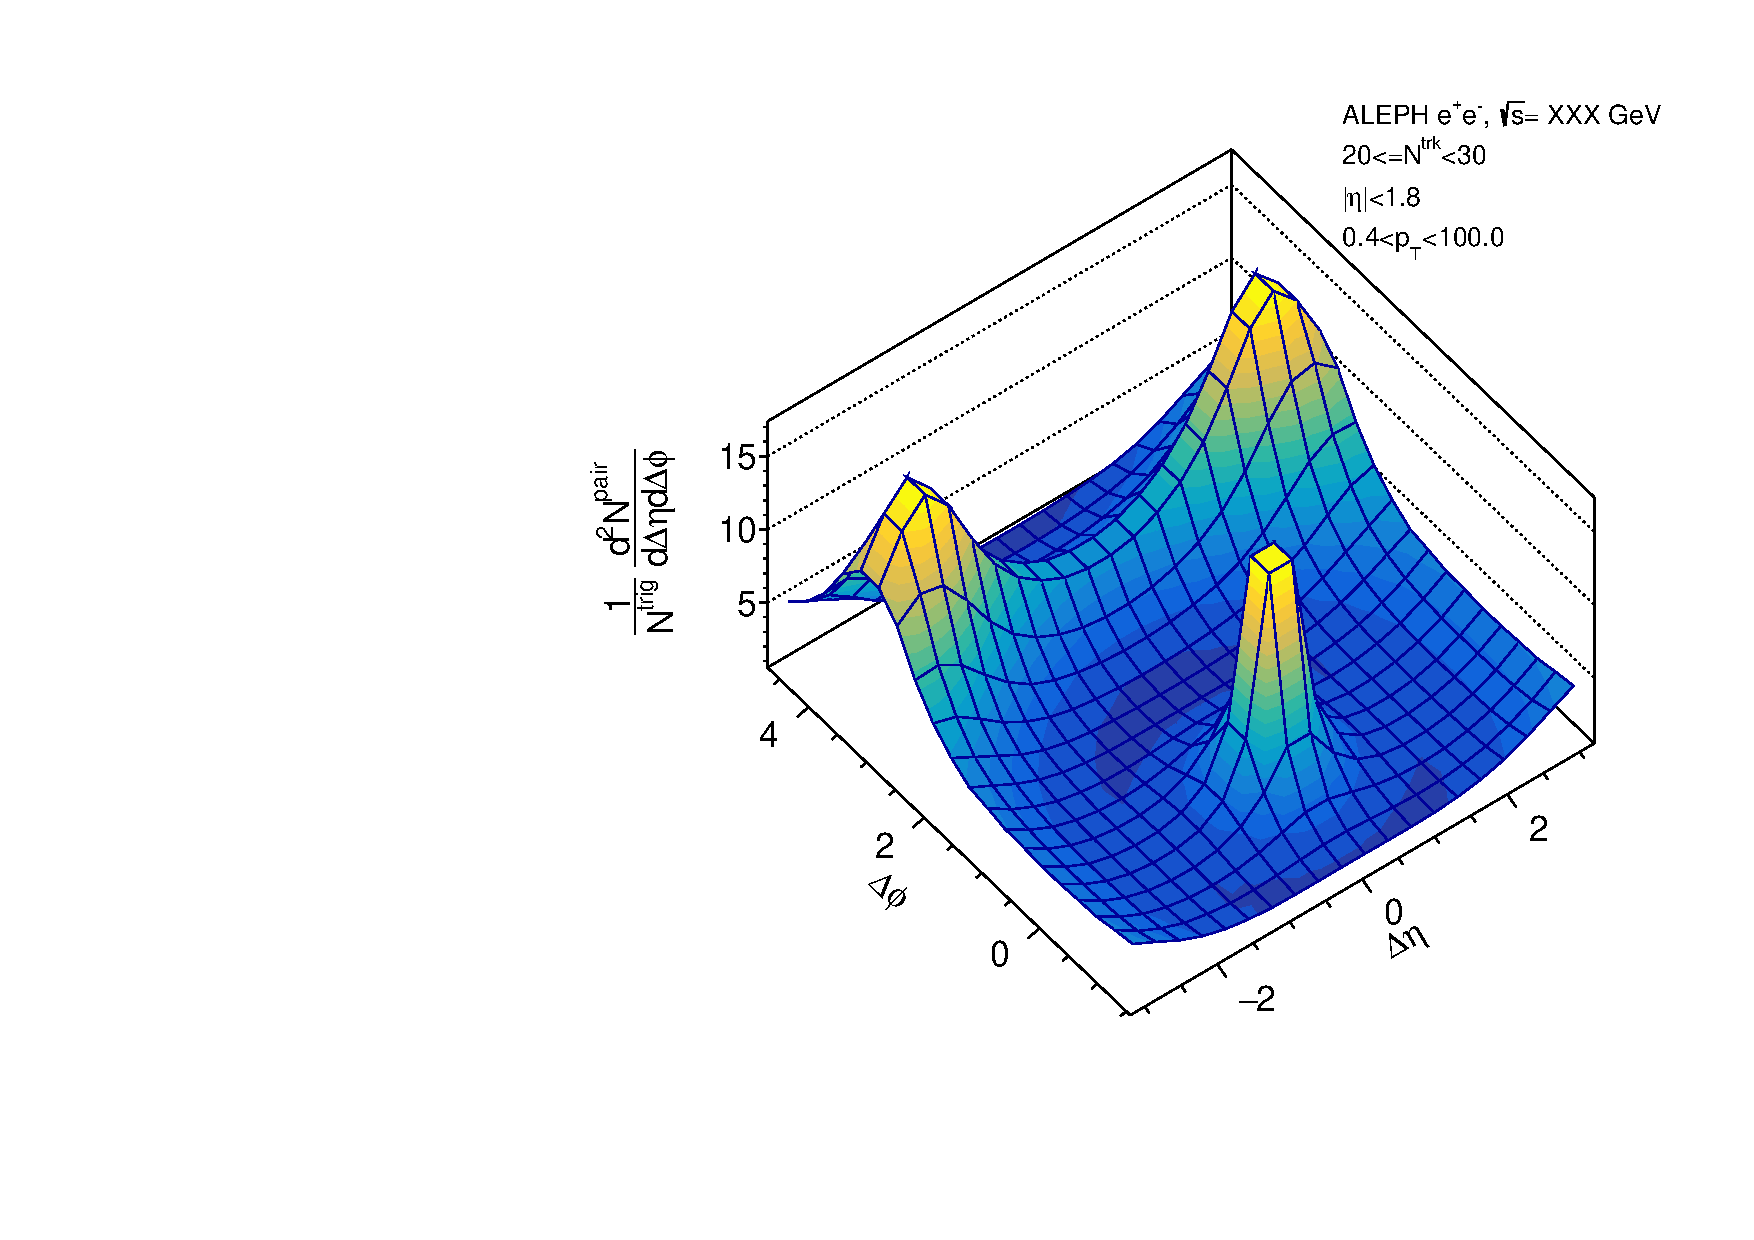
\includegraphics[width=.32\textwidth]{images/TwoParticleCorrelation/CrossCheck/20180126/LEP1_BEAM/LEP1_BEAM_ratio2_20_30.pdf}}\hfill
\subfloat{\label{sfig:e}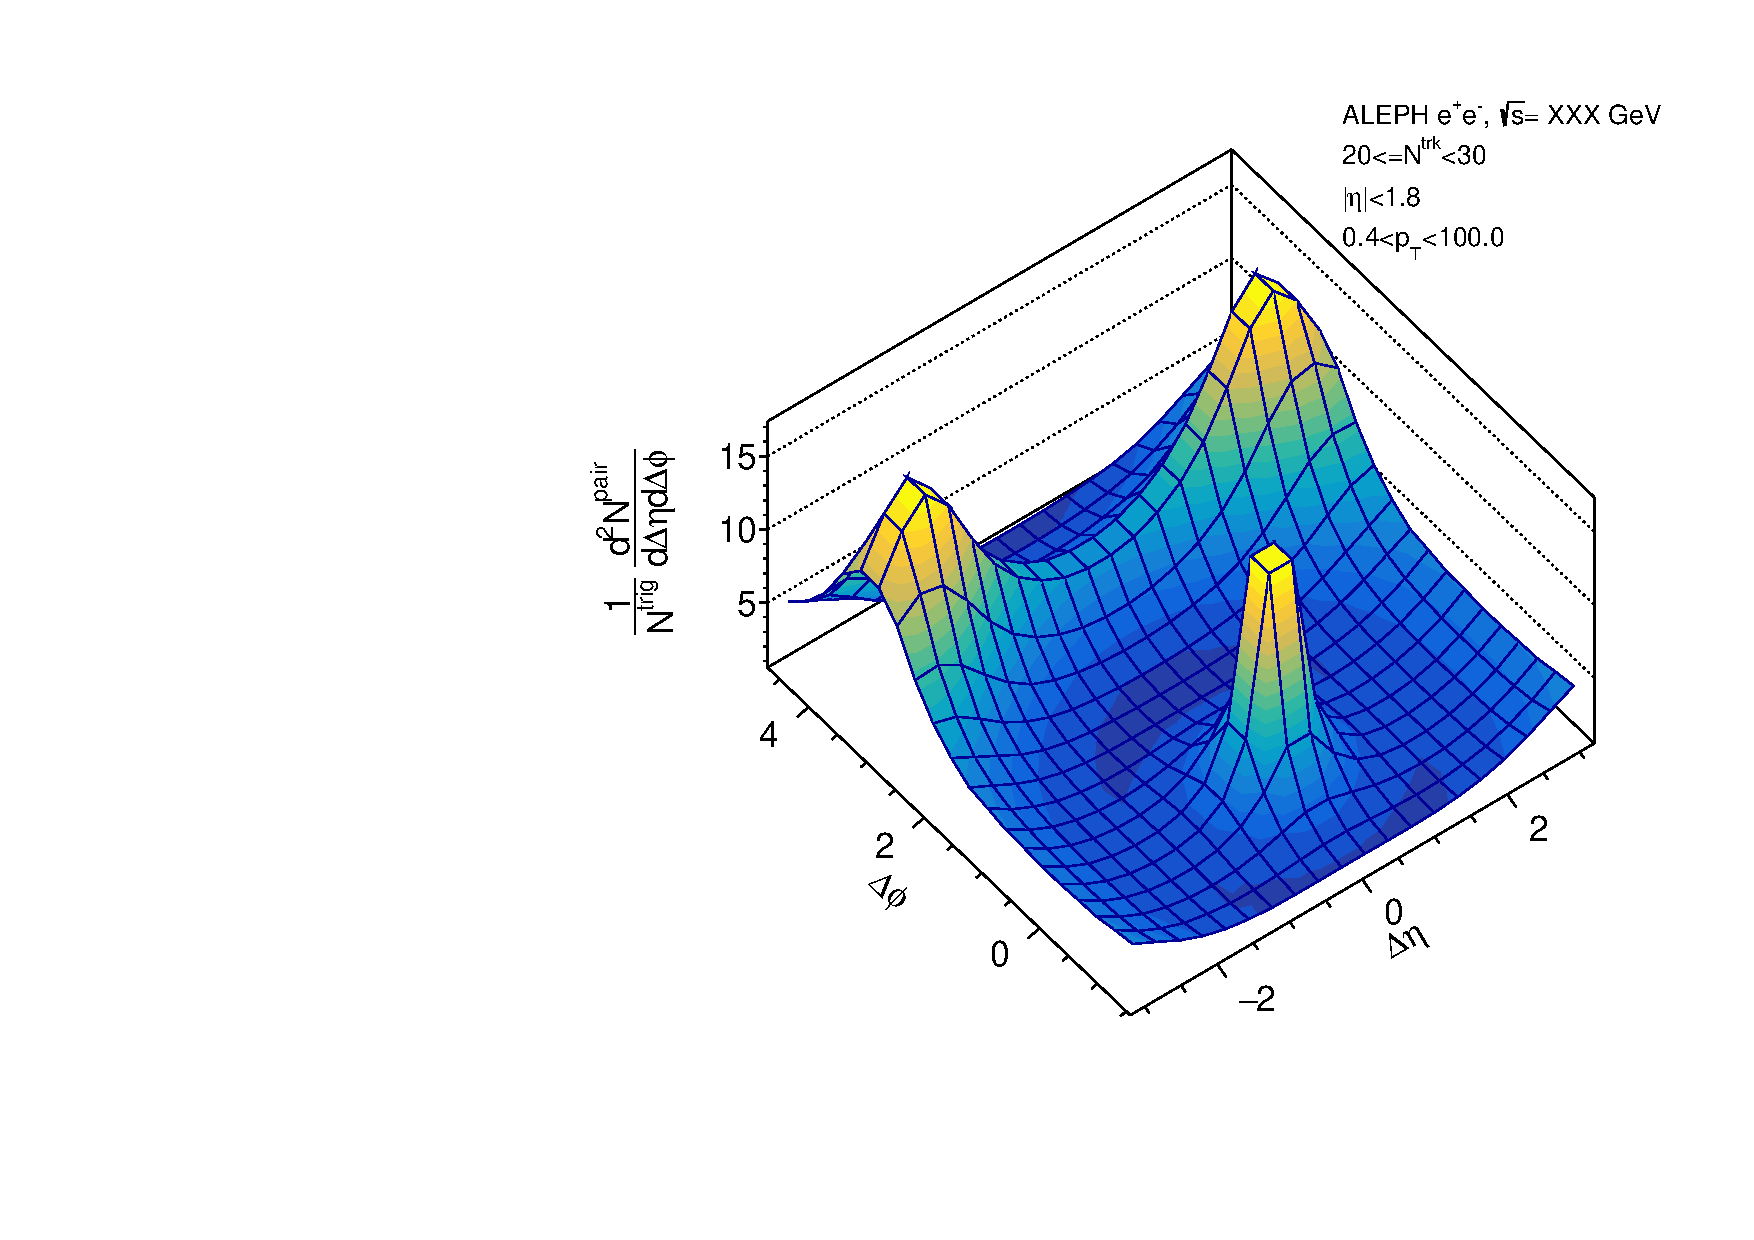
\includegraphics[width=.32\textwidth]{images/TwoParticleCorrelation/CrossCheck/20180126/LEP1_BEAM/LEP1_BEAM_ratio1_20_30.pdf}}\hfill
\subfloat{\label{sfig:f}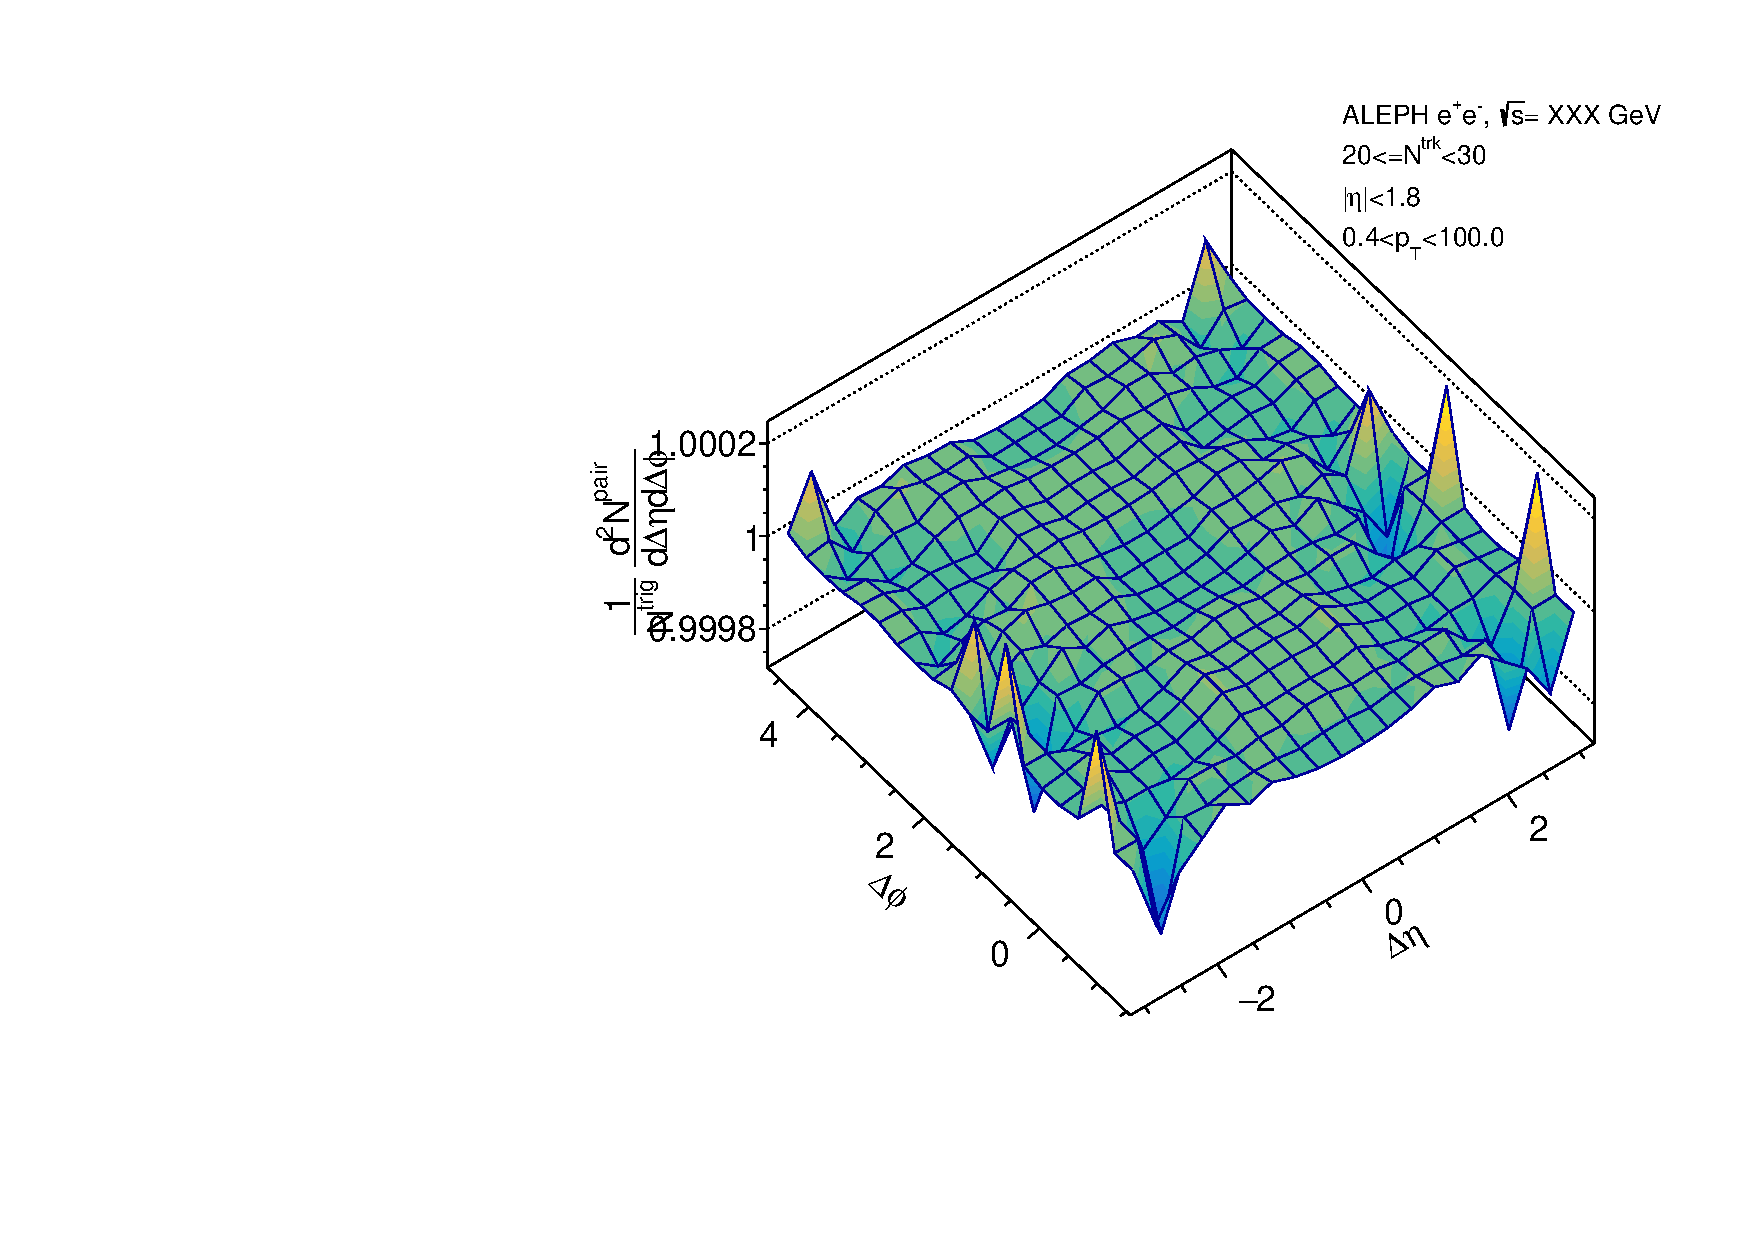
\includegraphics[width=.32\textwidth]{images/TwoParticleCorrelation/CrossCheck/20180126/LEP1_BEAM/LEP1_BEAM_r_ratio_20_30.pdf}}\hfill
\subfloat{\label{sfig:g}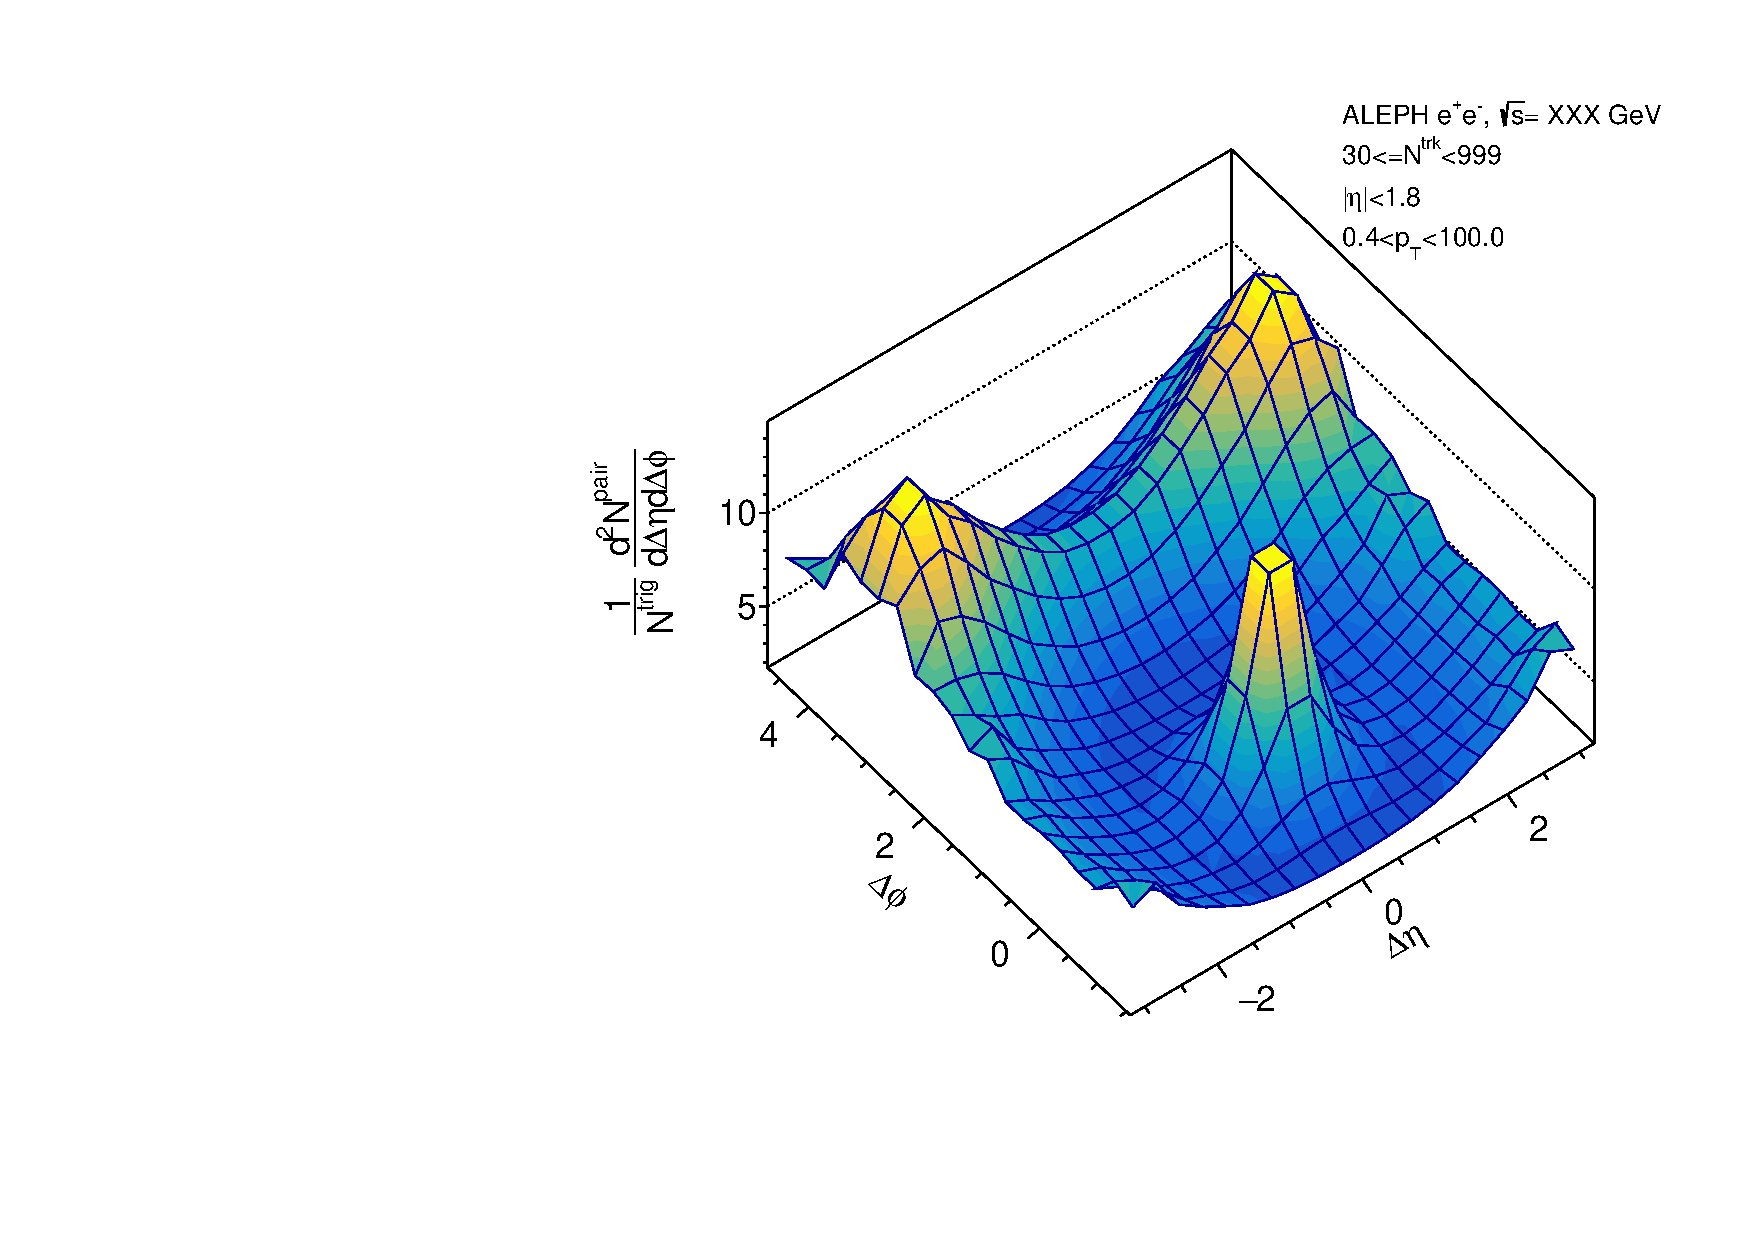
\includegraphics[width=.32\textwidth]{images/TwoParticleCorrelation/CrossCheck/20180126/LEP1_BEAM/LEP1_BEAM_ratio2_30_999.pdf}}\hfill
\subfloat{\label{sfig:h}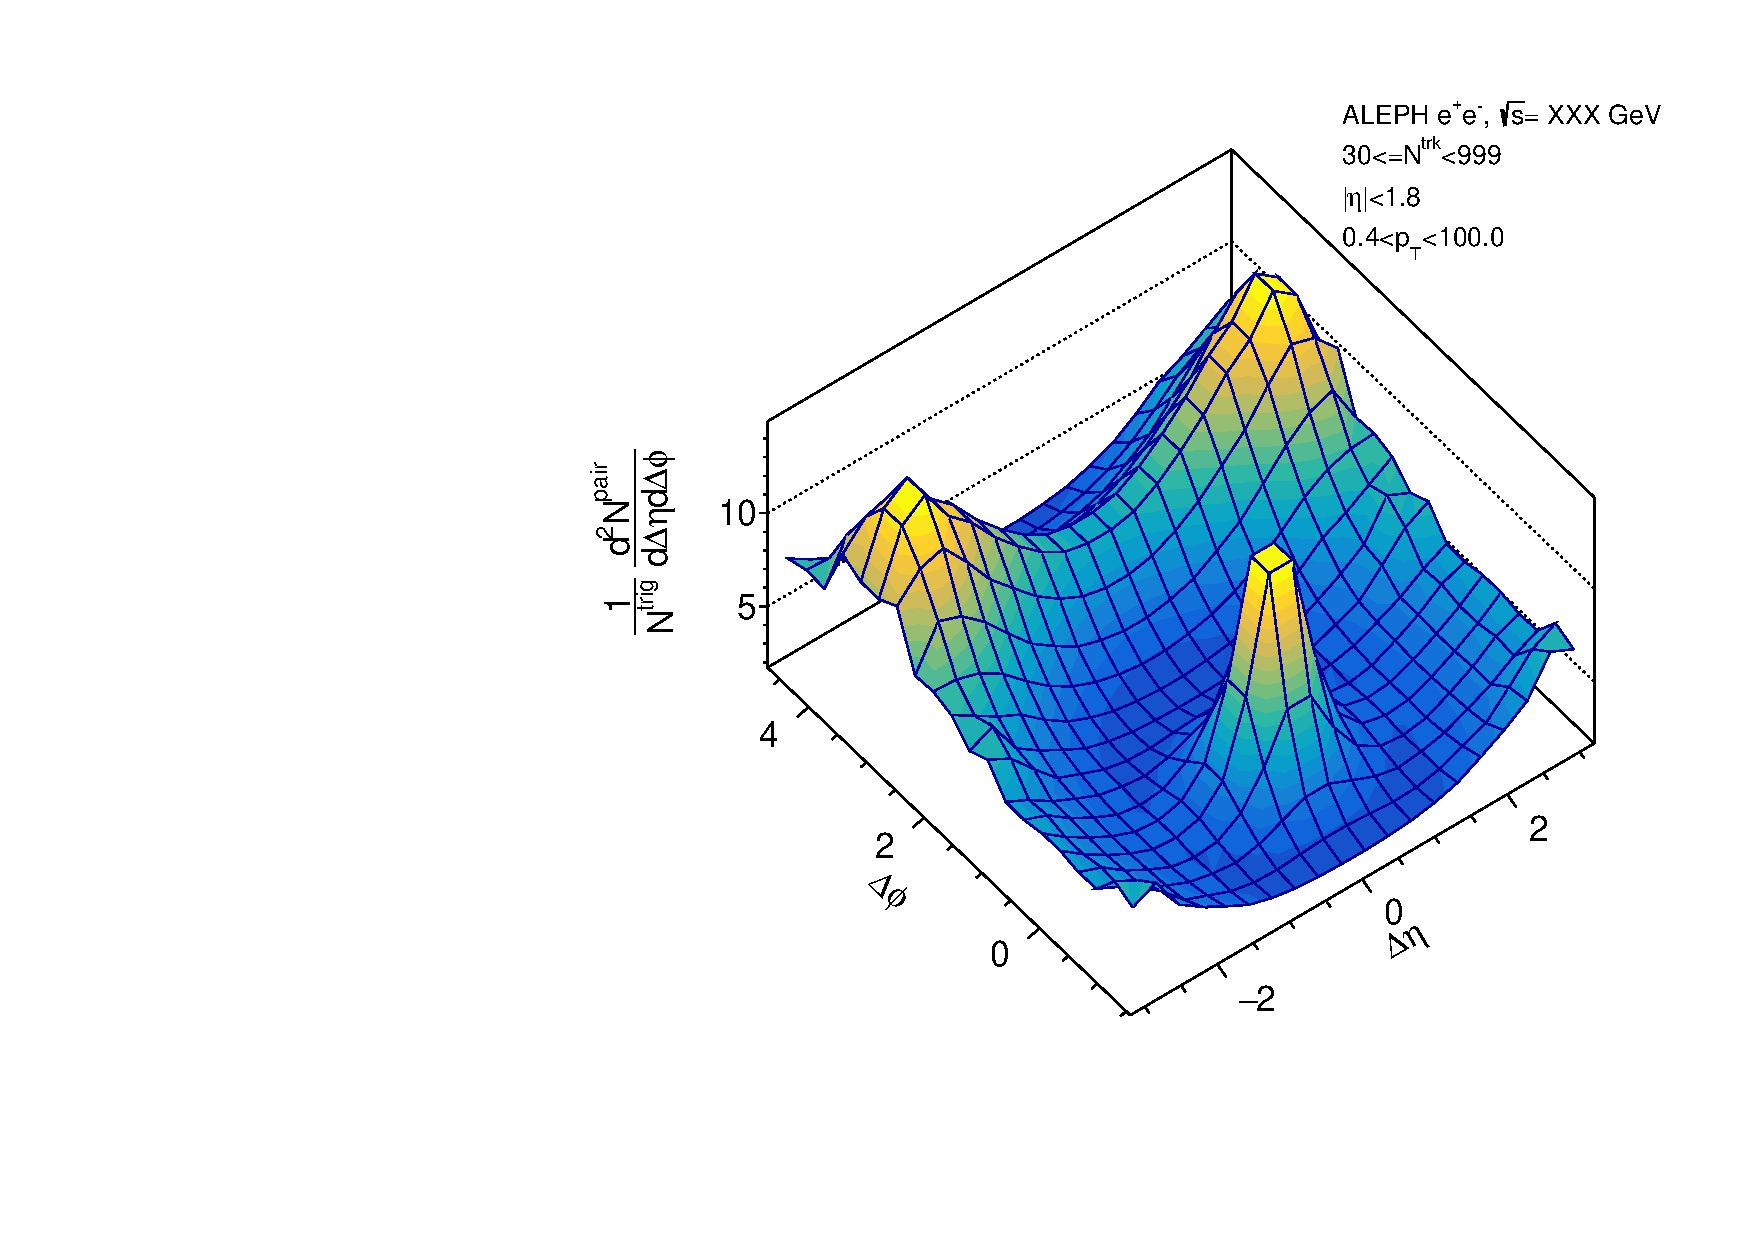
\includegraphics[width=.32\textwidth]{images/TwoParticleCorrelation/CrossCheck/20180126/LEP1_BEAM/LEP1_BEAM_ratio1_30_999.pdf}}\hfill
\subfloat{\label{sfig:i}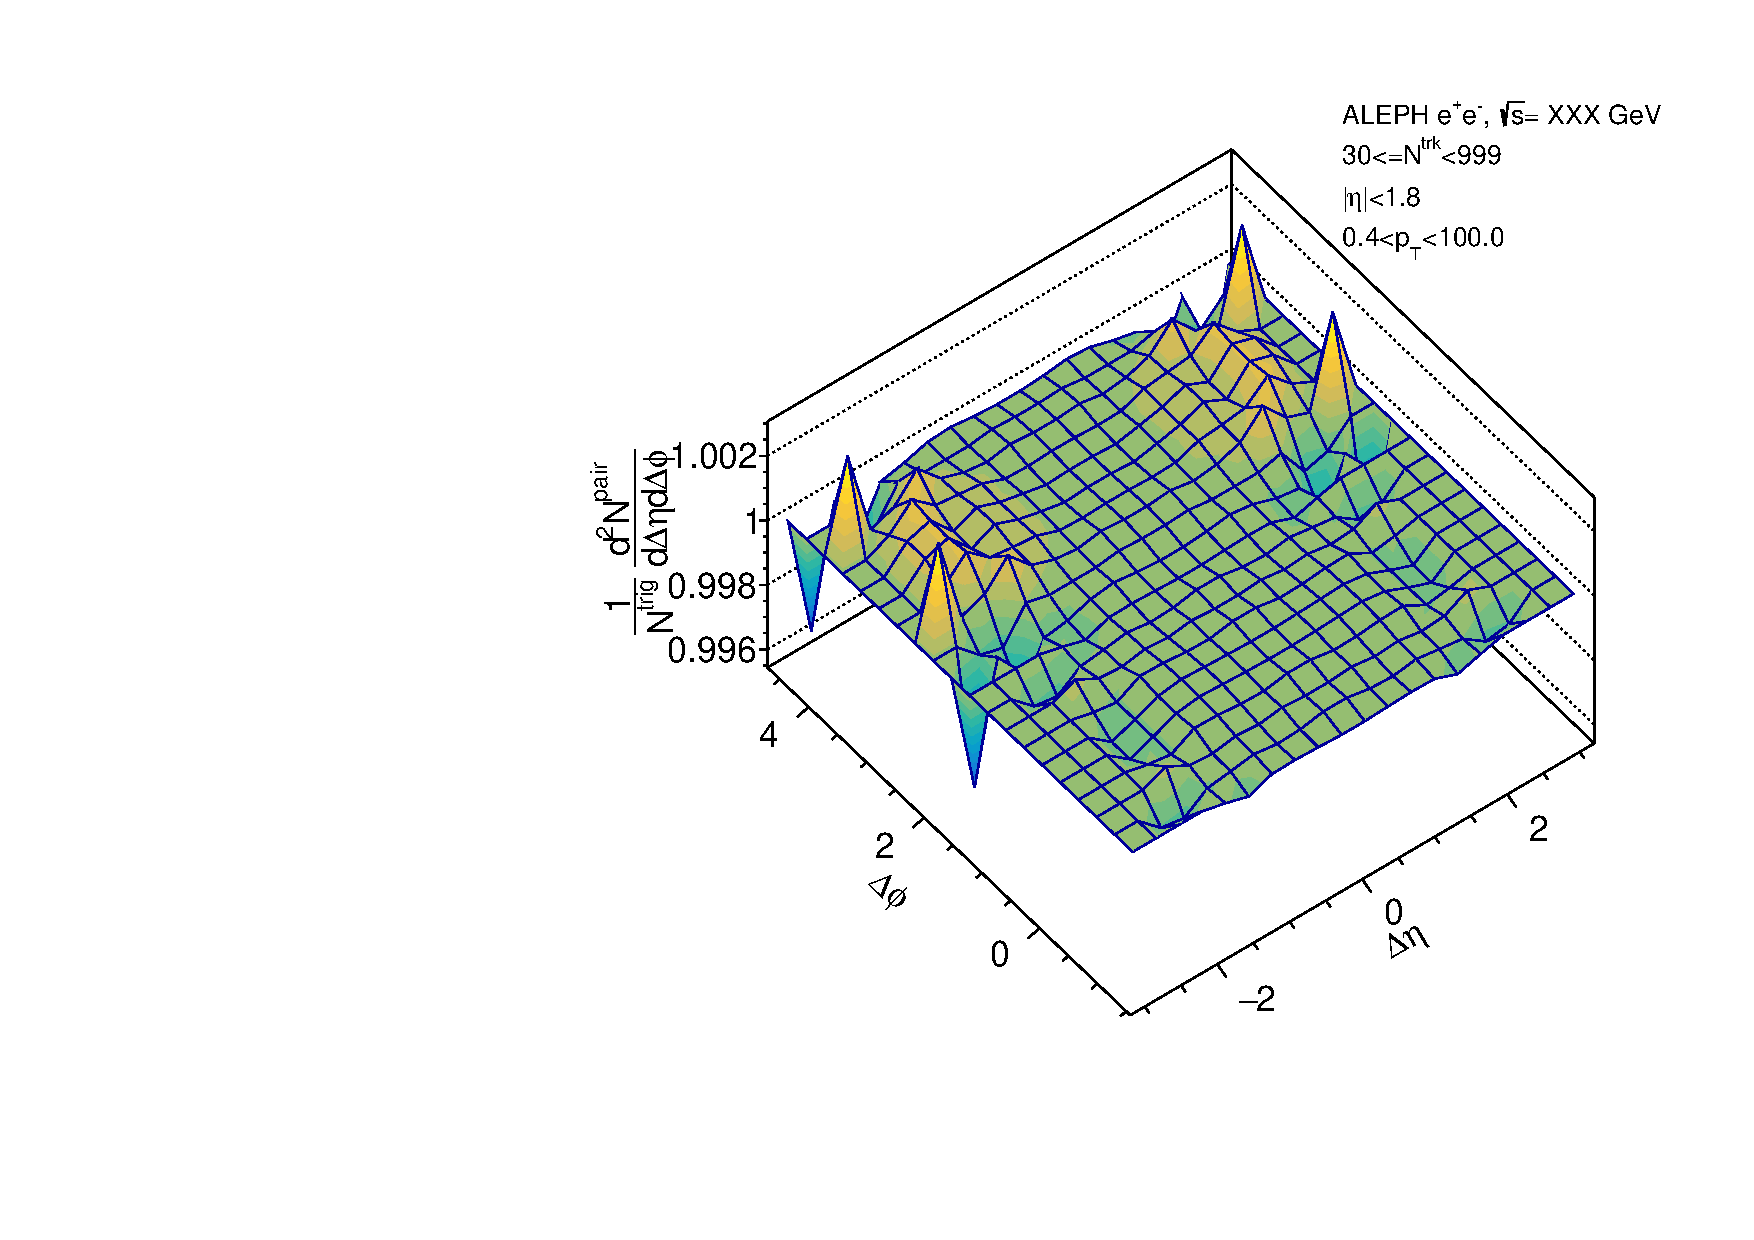
\includegraphics[width=.32\textwidth]{images/TwoParticleCorrelation/CrossCheck/20180126/LEP1_BEAM/LEP1_BEAM_r_ratio_30_999.pdf}} \\
\caption{Two particle correlation fuctions for the LEP1 data set analyzed in the beam axis.}
\label{fig:test}
\end{figure}

\begin{figure}[H]
\centering
\subfloat{\label{sfig:a}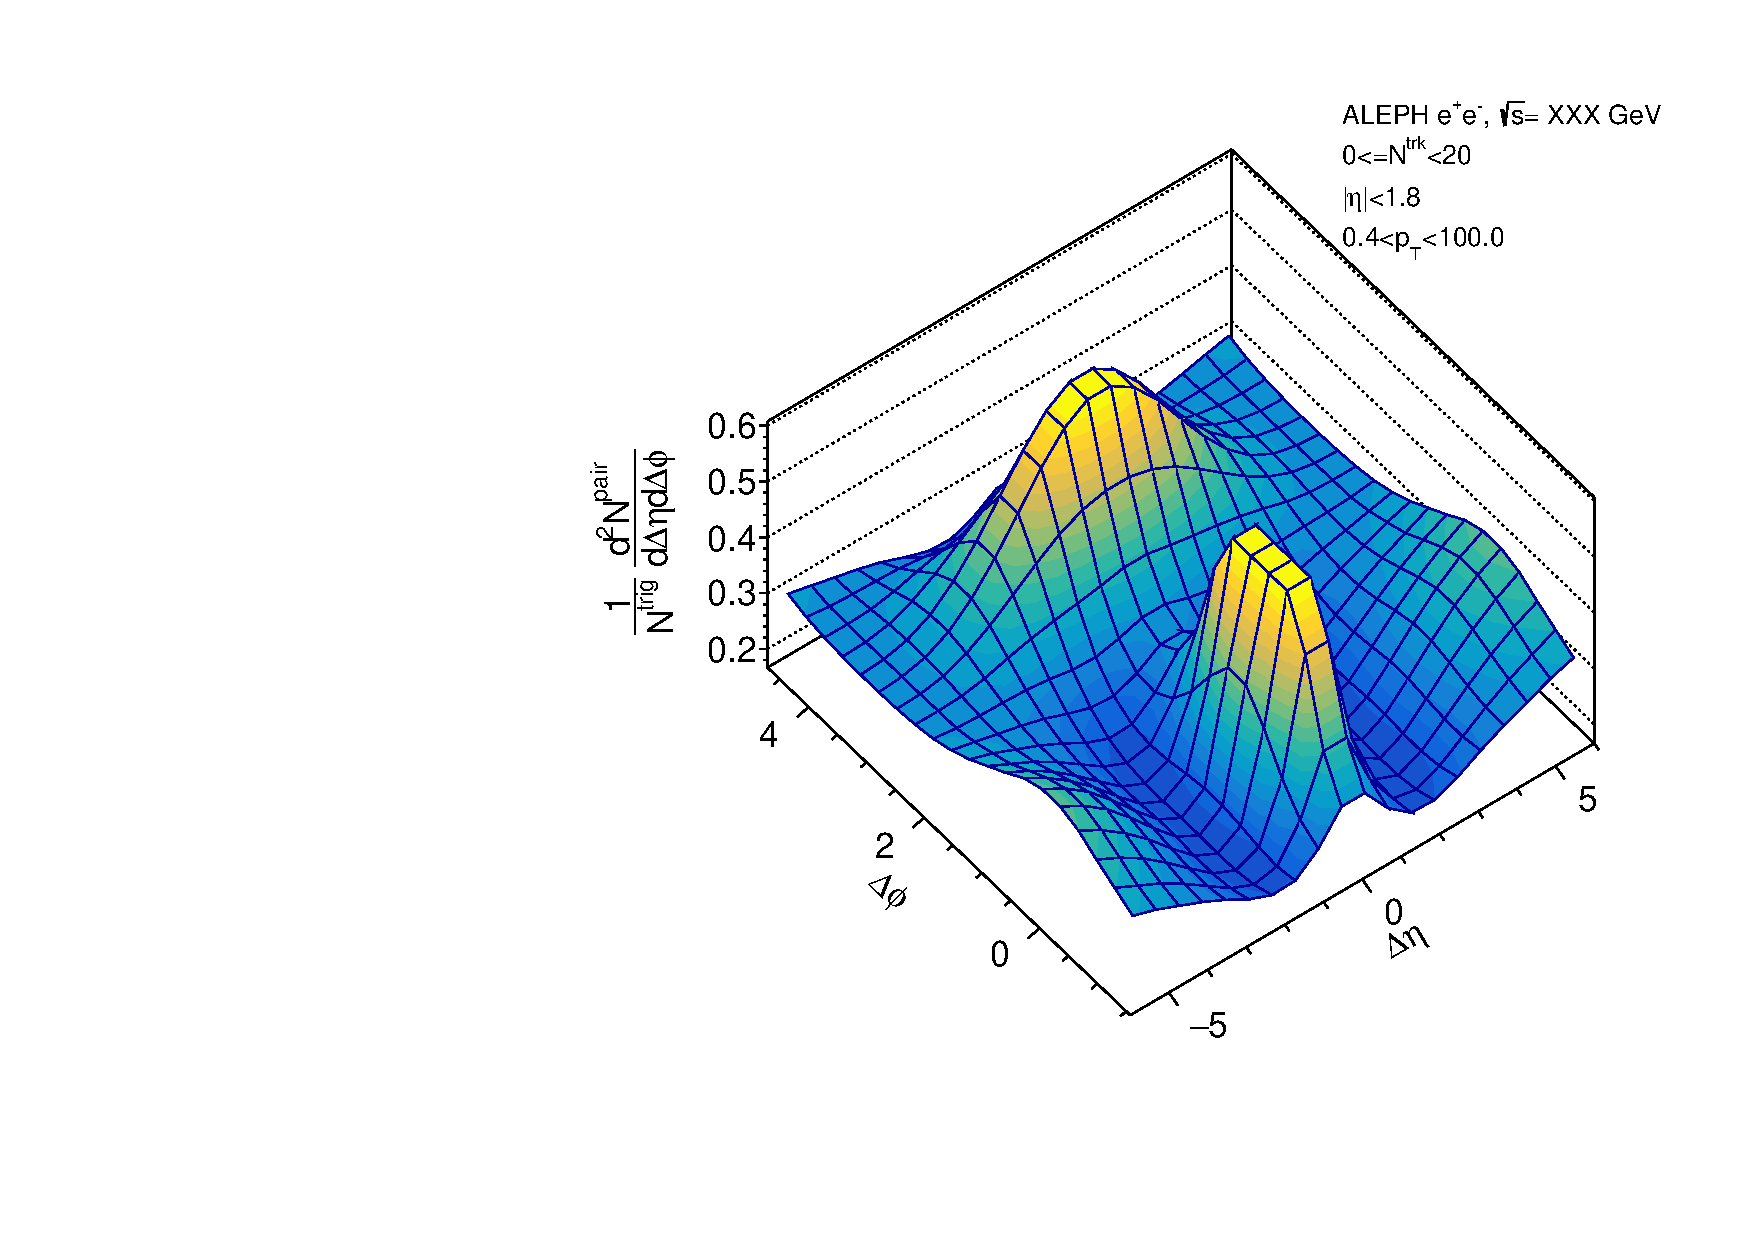
\includegraphics[width=.32\textwidth]{images/TwoParticleCorrelation/CrossCheck/20180126/LEP1_THRUST/LEP1_THRUST_ratio2_0_20.pdf}}\hfill
\subfloat{\label{sfig:b}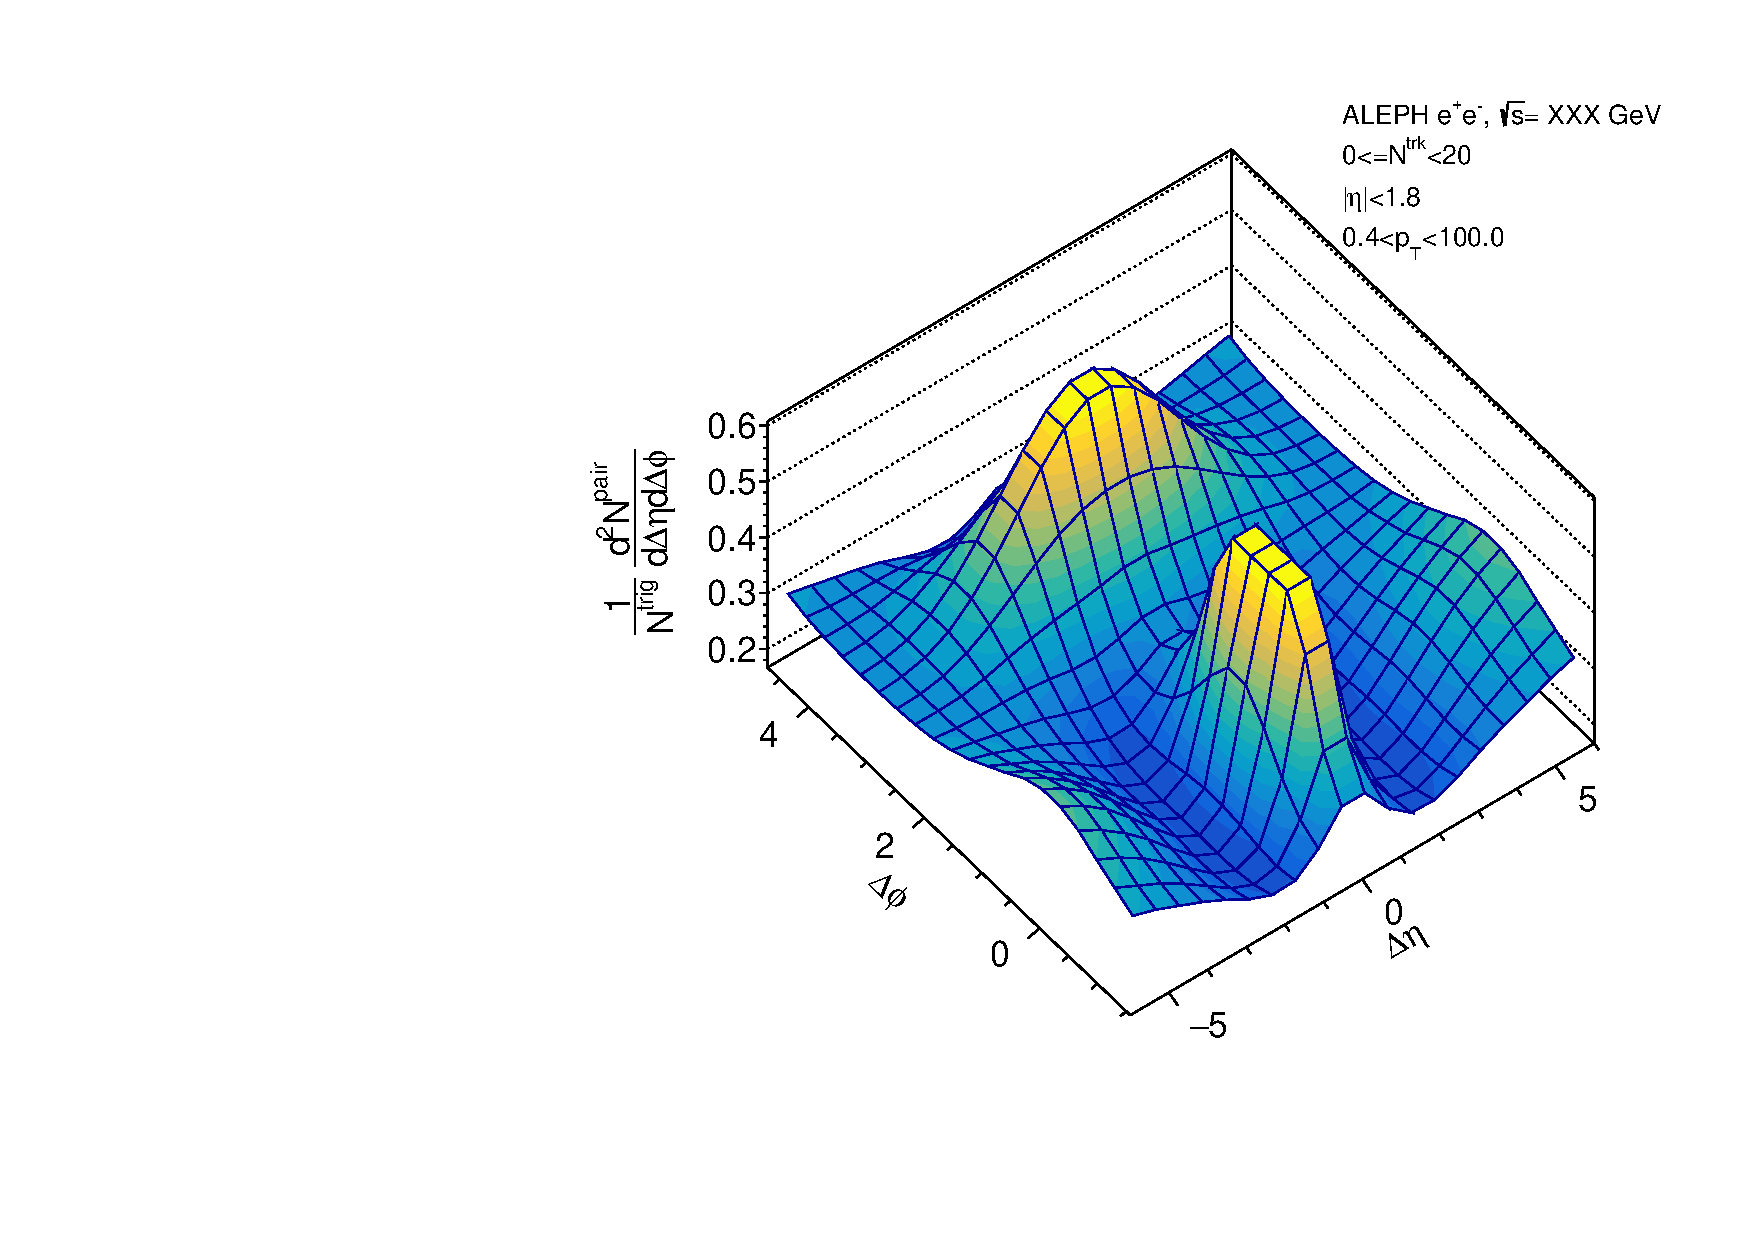
\includegraphics[width=.32\textwidth]{images/TwoParticleCorrelation/CrossCheck/20180126/LEP1_THRUST/LEP1_THRUST_ratio1_0_20.pdf}}\hfill
\subfloat{\label{sfig:c}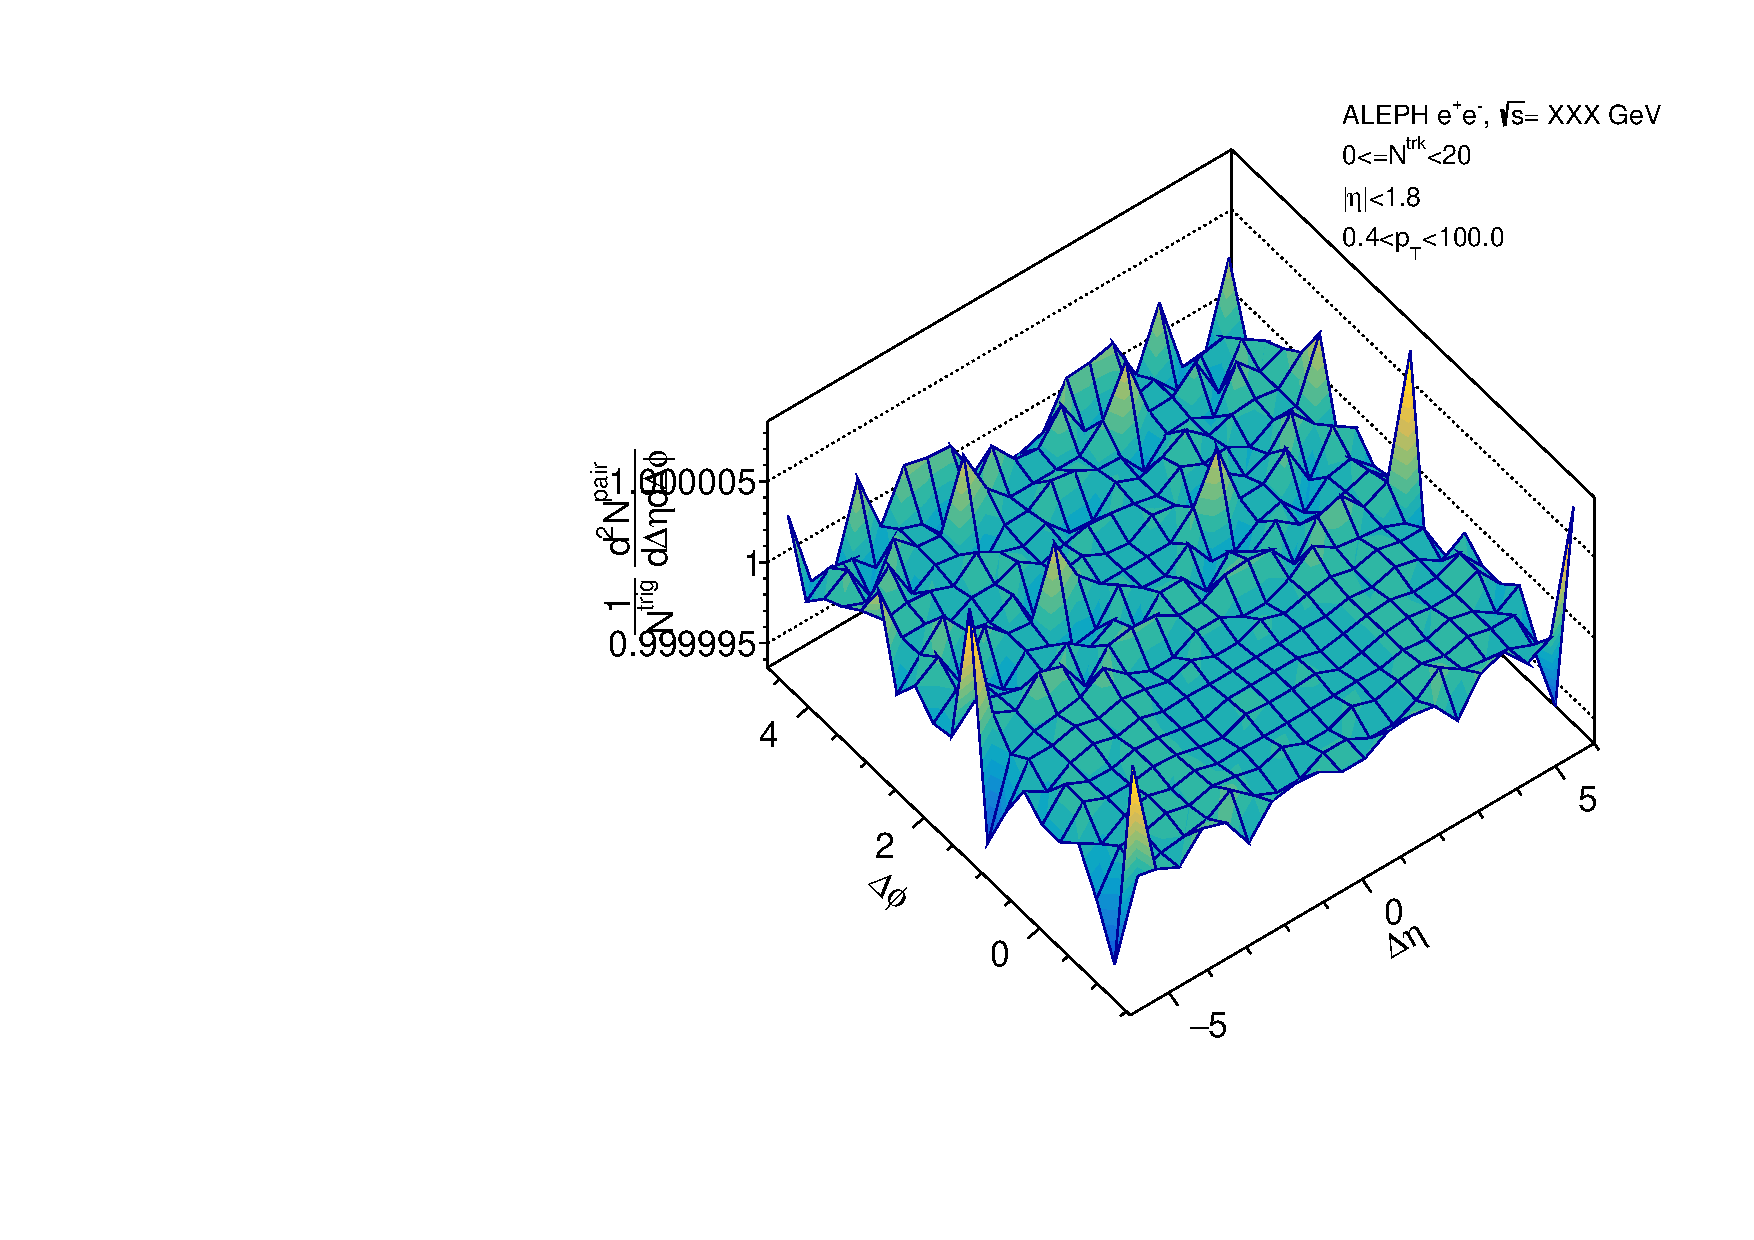
\includegraphics[width=.32\textwidth]{images/TwoParticleCorrelation/CrossCheck/20180126/LEP1_THRUST/LEP1_THRUST_r_ratio_0_20.pdf}}\hfill
\subfloat{\label{sfig:d}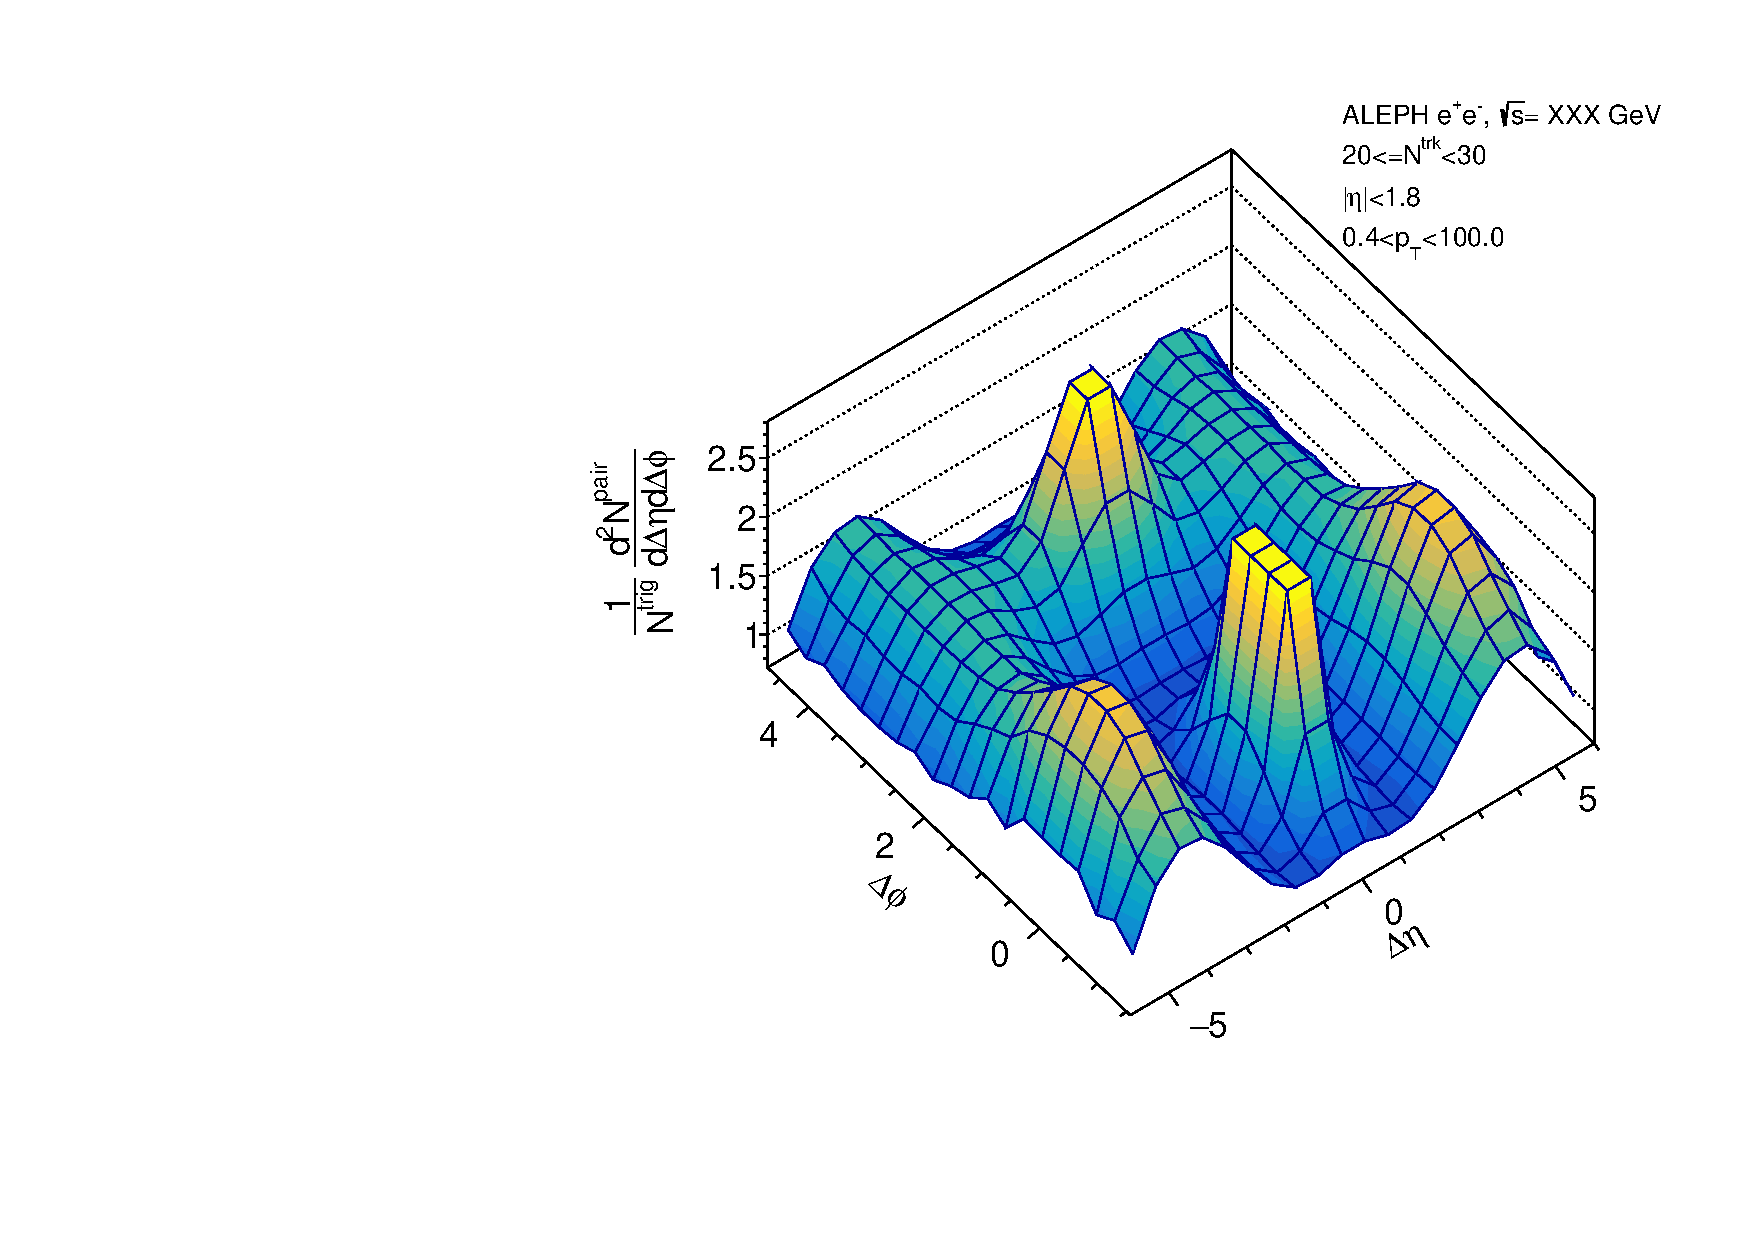
\includegraphics[width=.32\textwidth]{images/TwoParticleCorrelation/CrossCheck/20180126/LEP1_THRUST/LEP1_THRUST_ratio2_20_30.pdf}}\hfill
\subfloat{\label{sfig:e}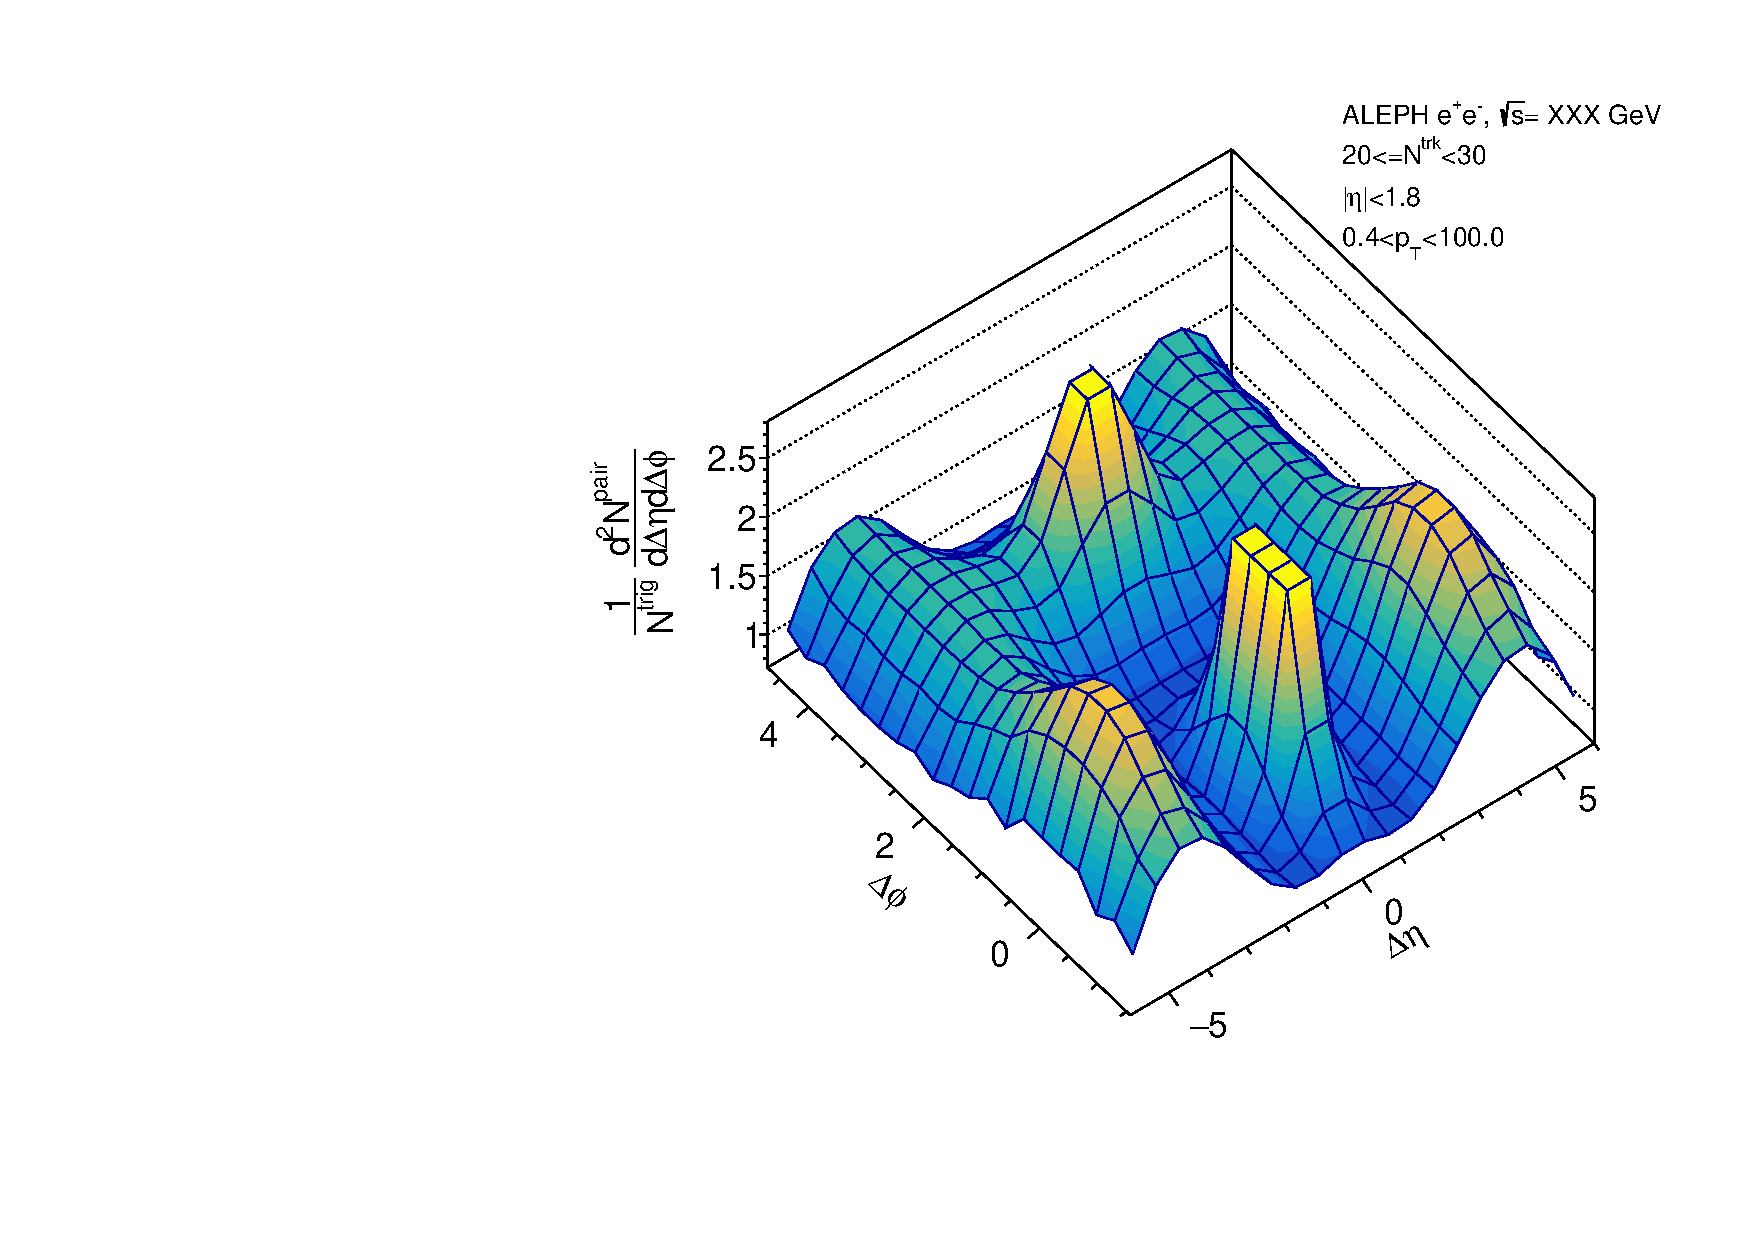
\includegraphics[width=.32\textwidth]{images/TwoParticleCorrelation/CrossCheck/20180126/LEP1_THRUST/LEP1_THRUST_ratio1_20_30.pdf}}\hfill
\subfloat{\label{sfig:f}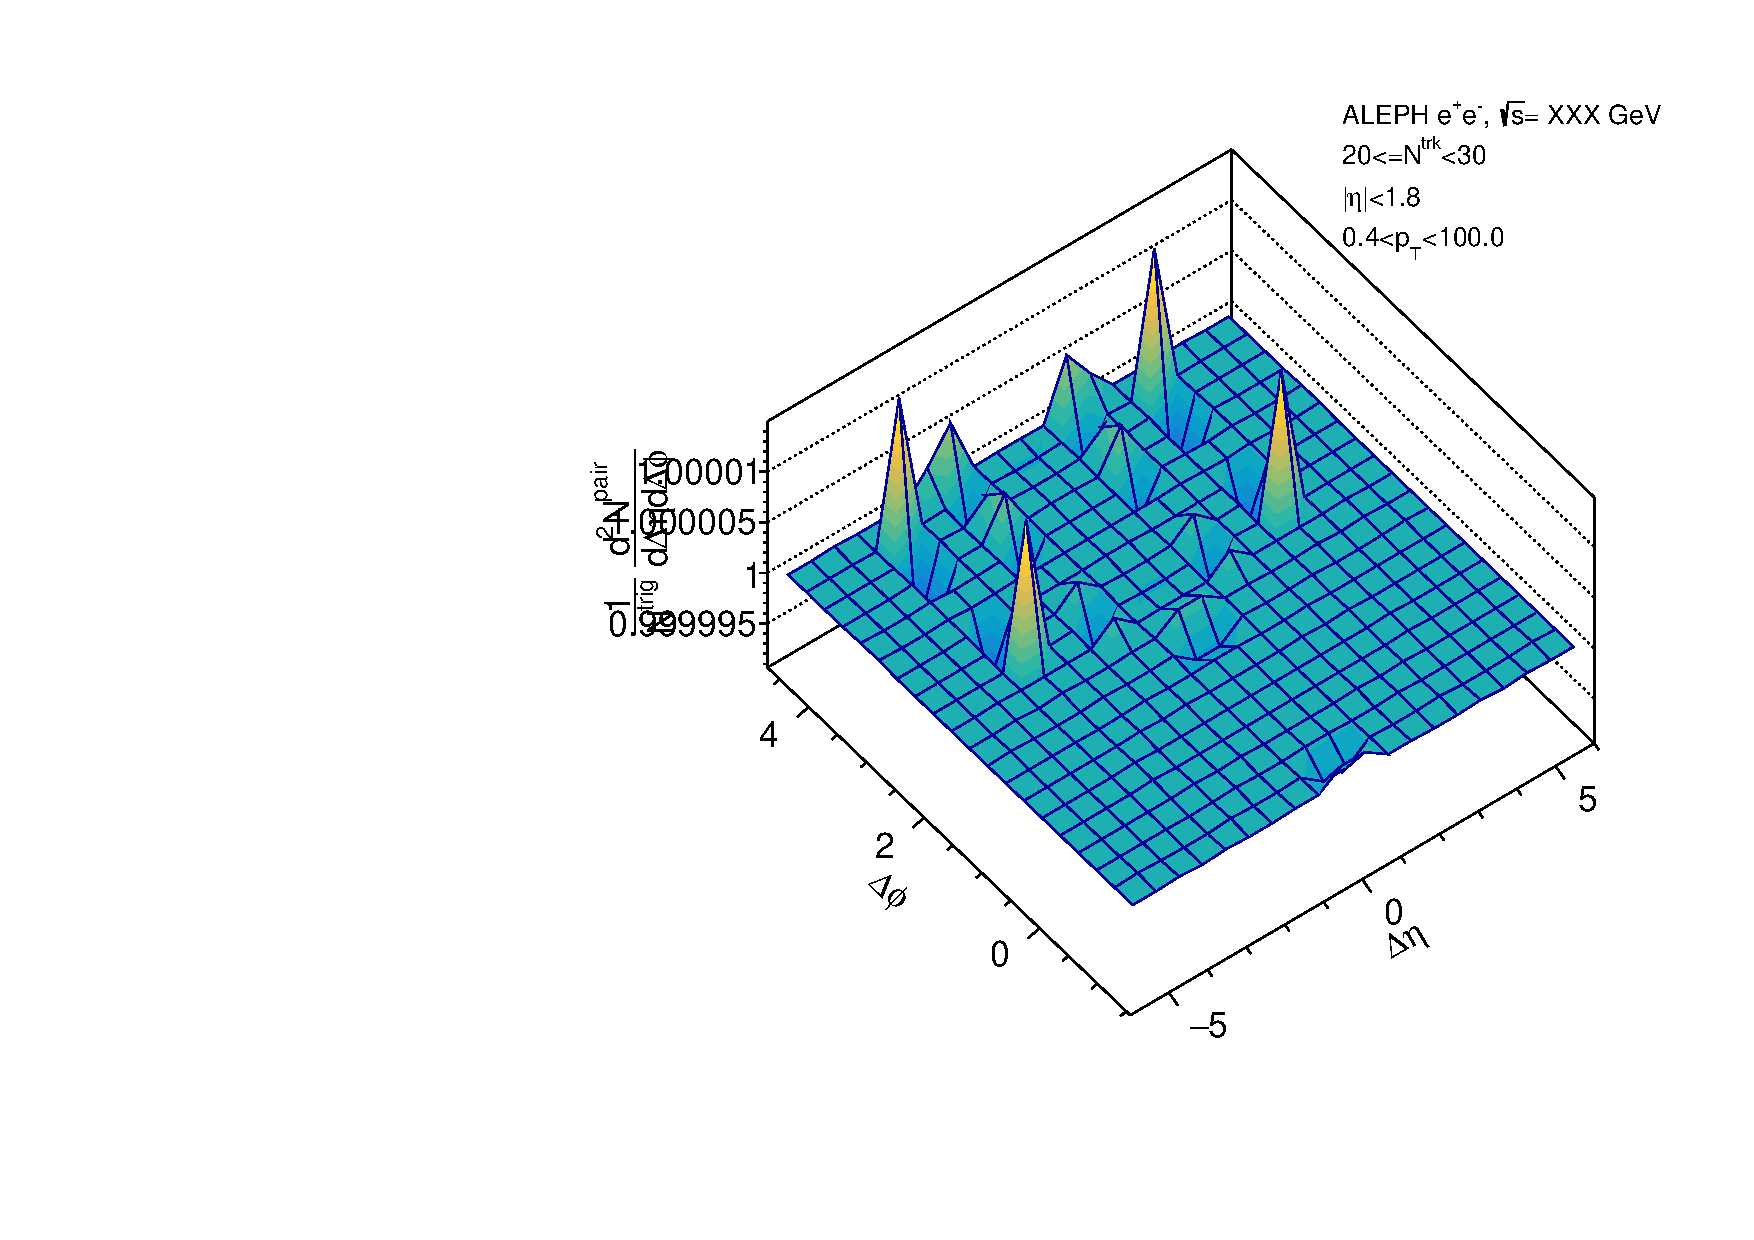
\includegraphics[width=.32\textwidth]{images/TwoParticleCorrelation/CrossCheck/20180126/LEP1_THRUST/LEP1_THRUST_r_ratio_20_30.pdf}}\hfill
\subfloat{\label{sfig:g}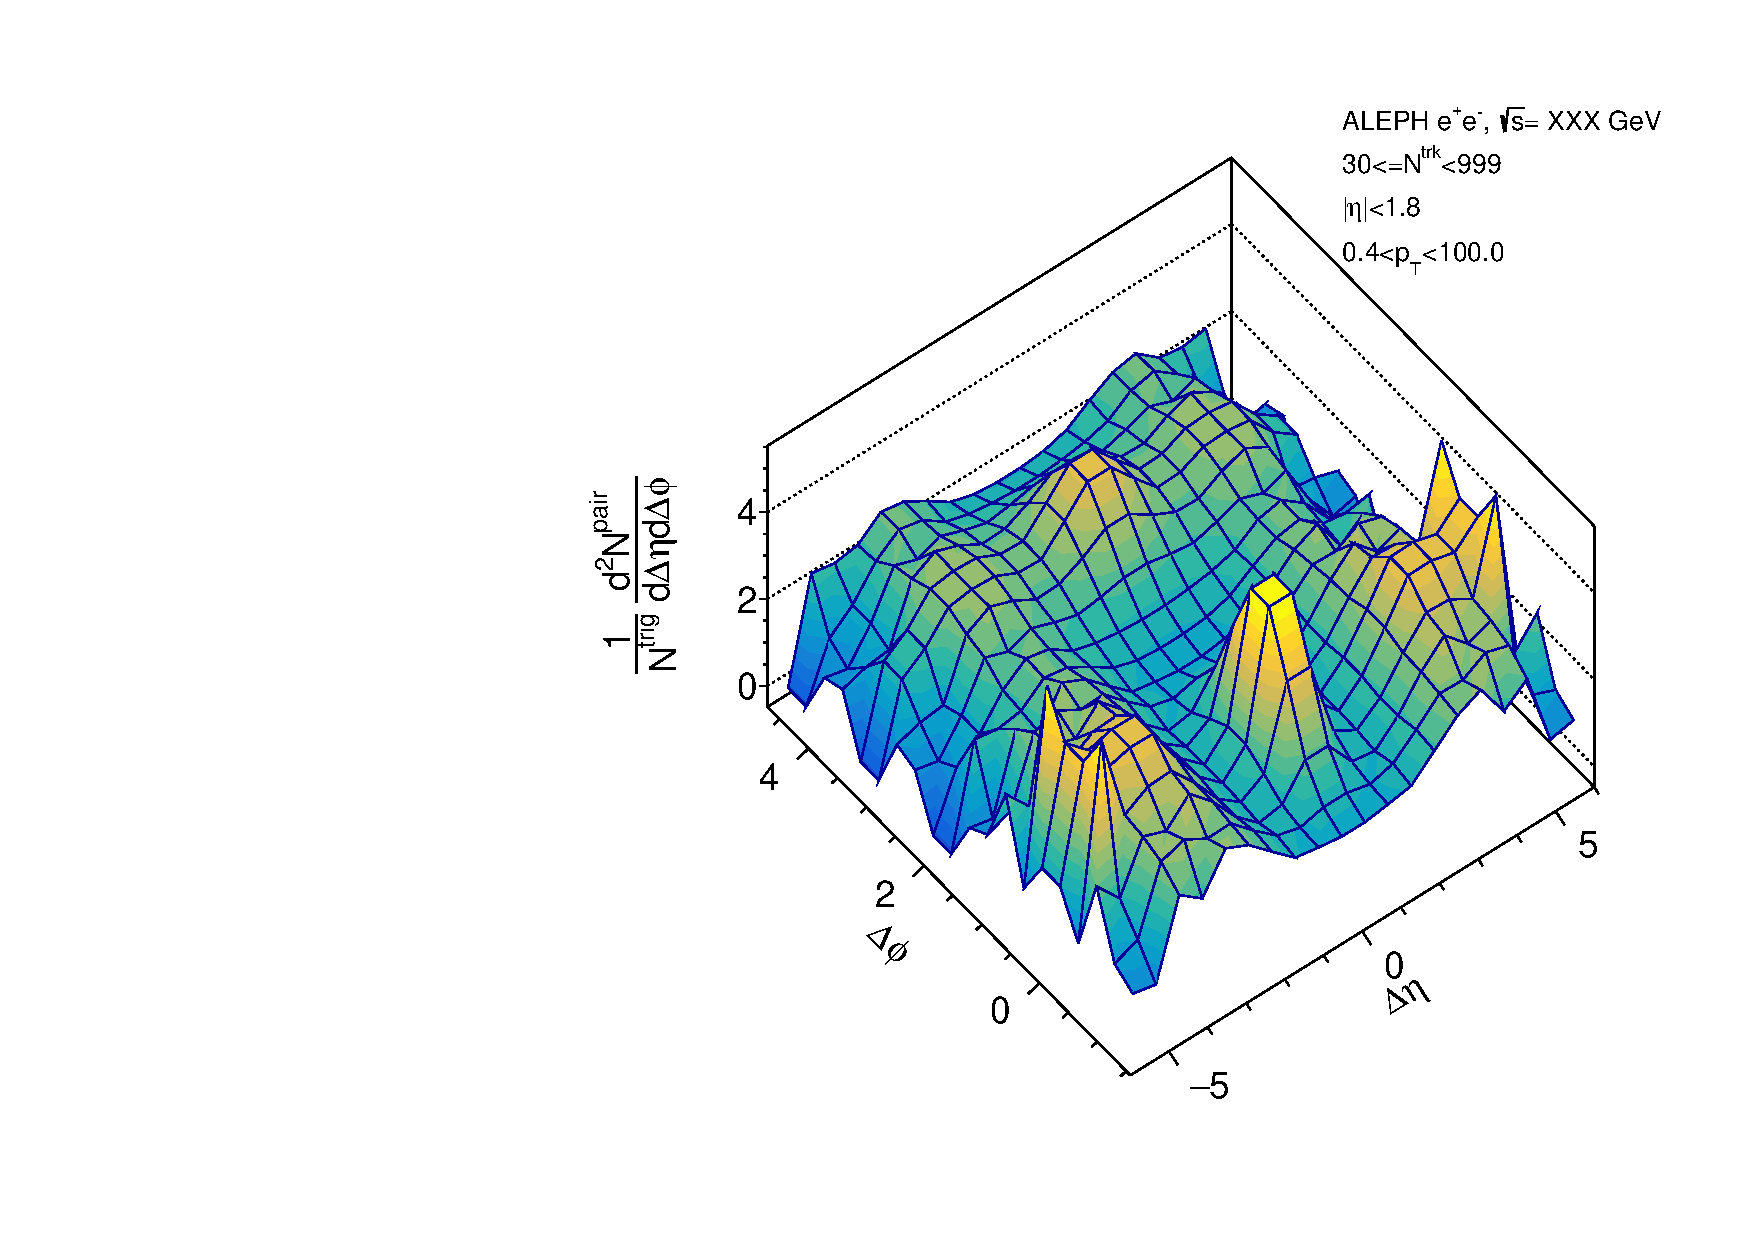
\includegraphics[width=.32\textwidth]{images/TwoParticleCorrelation/CrossCheck/20180126/LEP1_THRUST/LEP1_THRUST_ratio2_30_999.pdf}}\hfill
\subfloat{\label{sfig:h}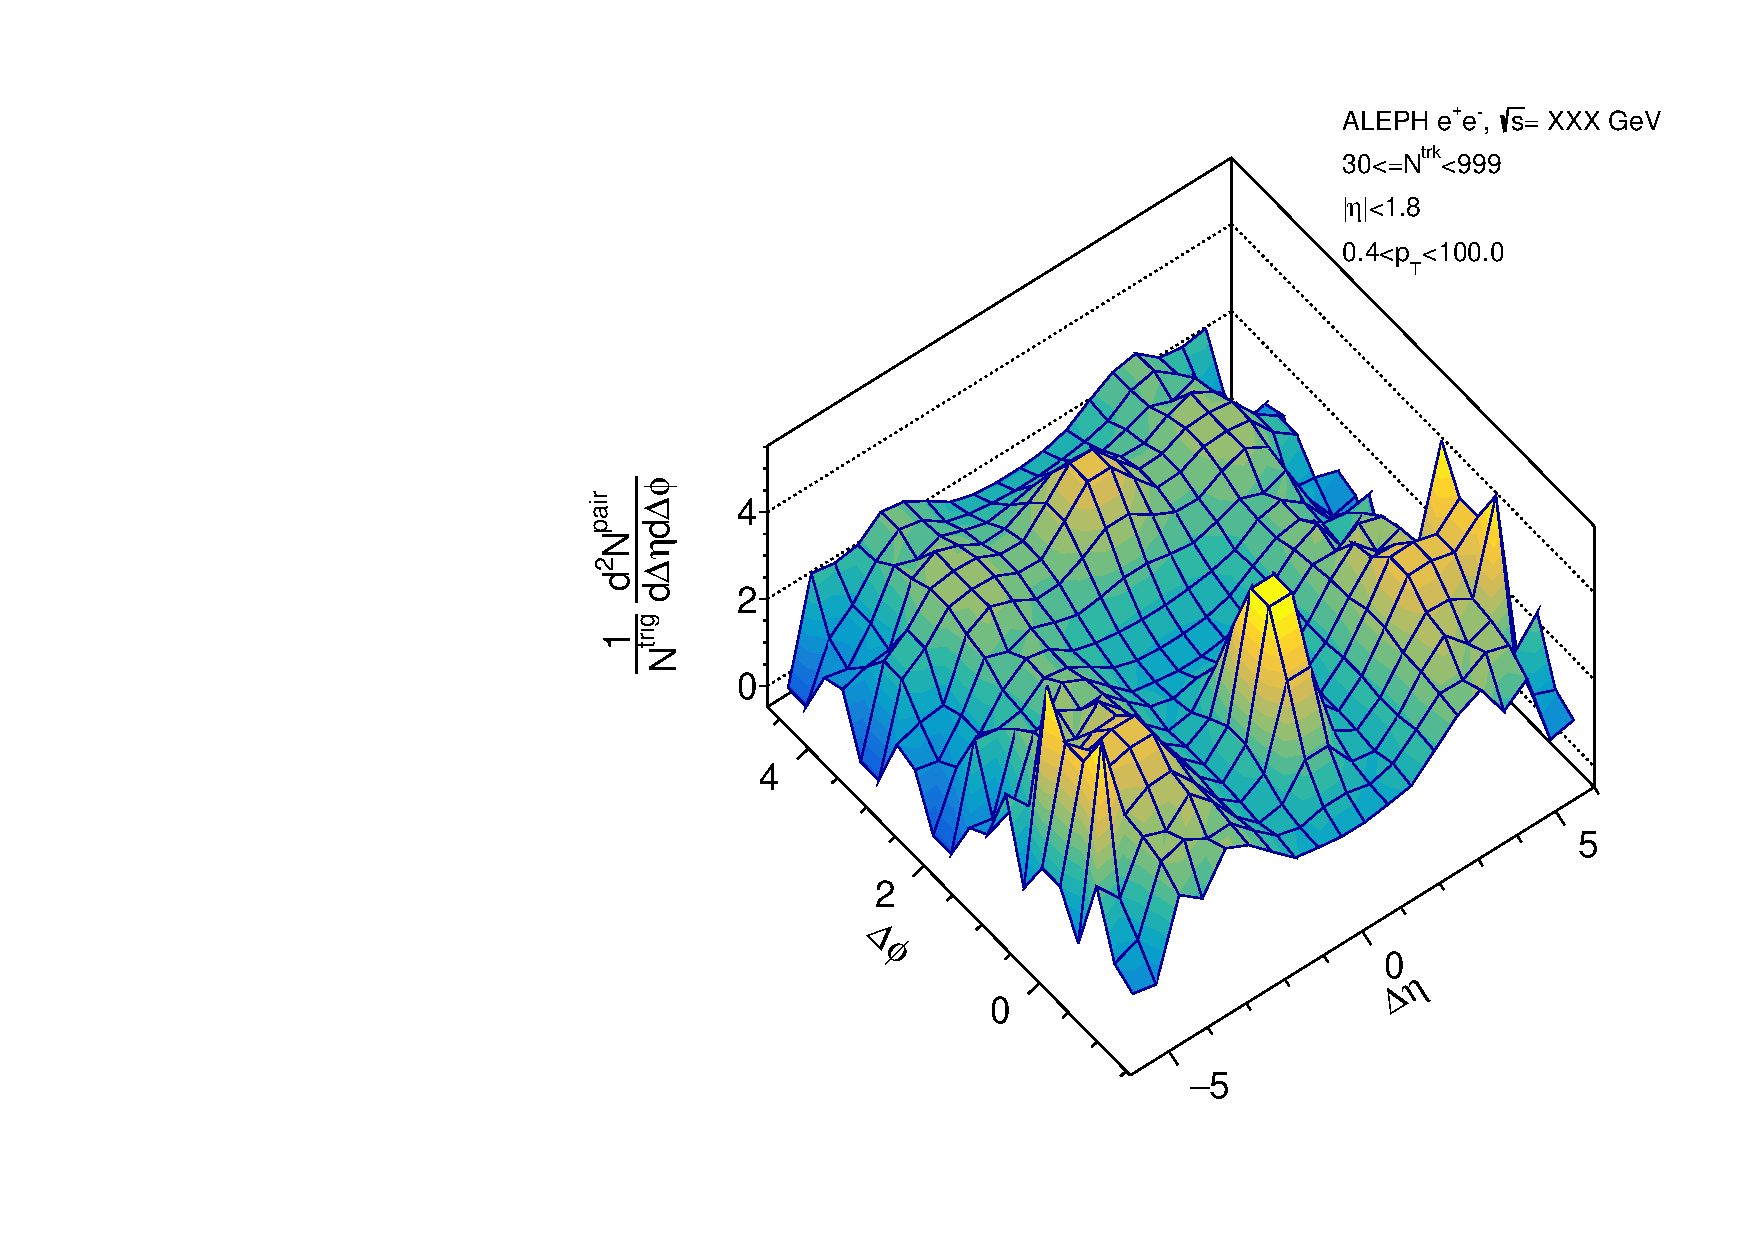
\includegraphics[width=.32\textwidth]{images/TwoParticleCorrelation/CrossCheck/20180126/LEP1_THRUST/LEP1_THRUST_ratio1_30_999.pdf}}\hfill
\subfloat{\label{sfig:i}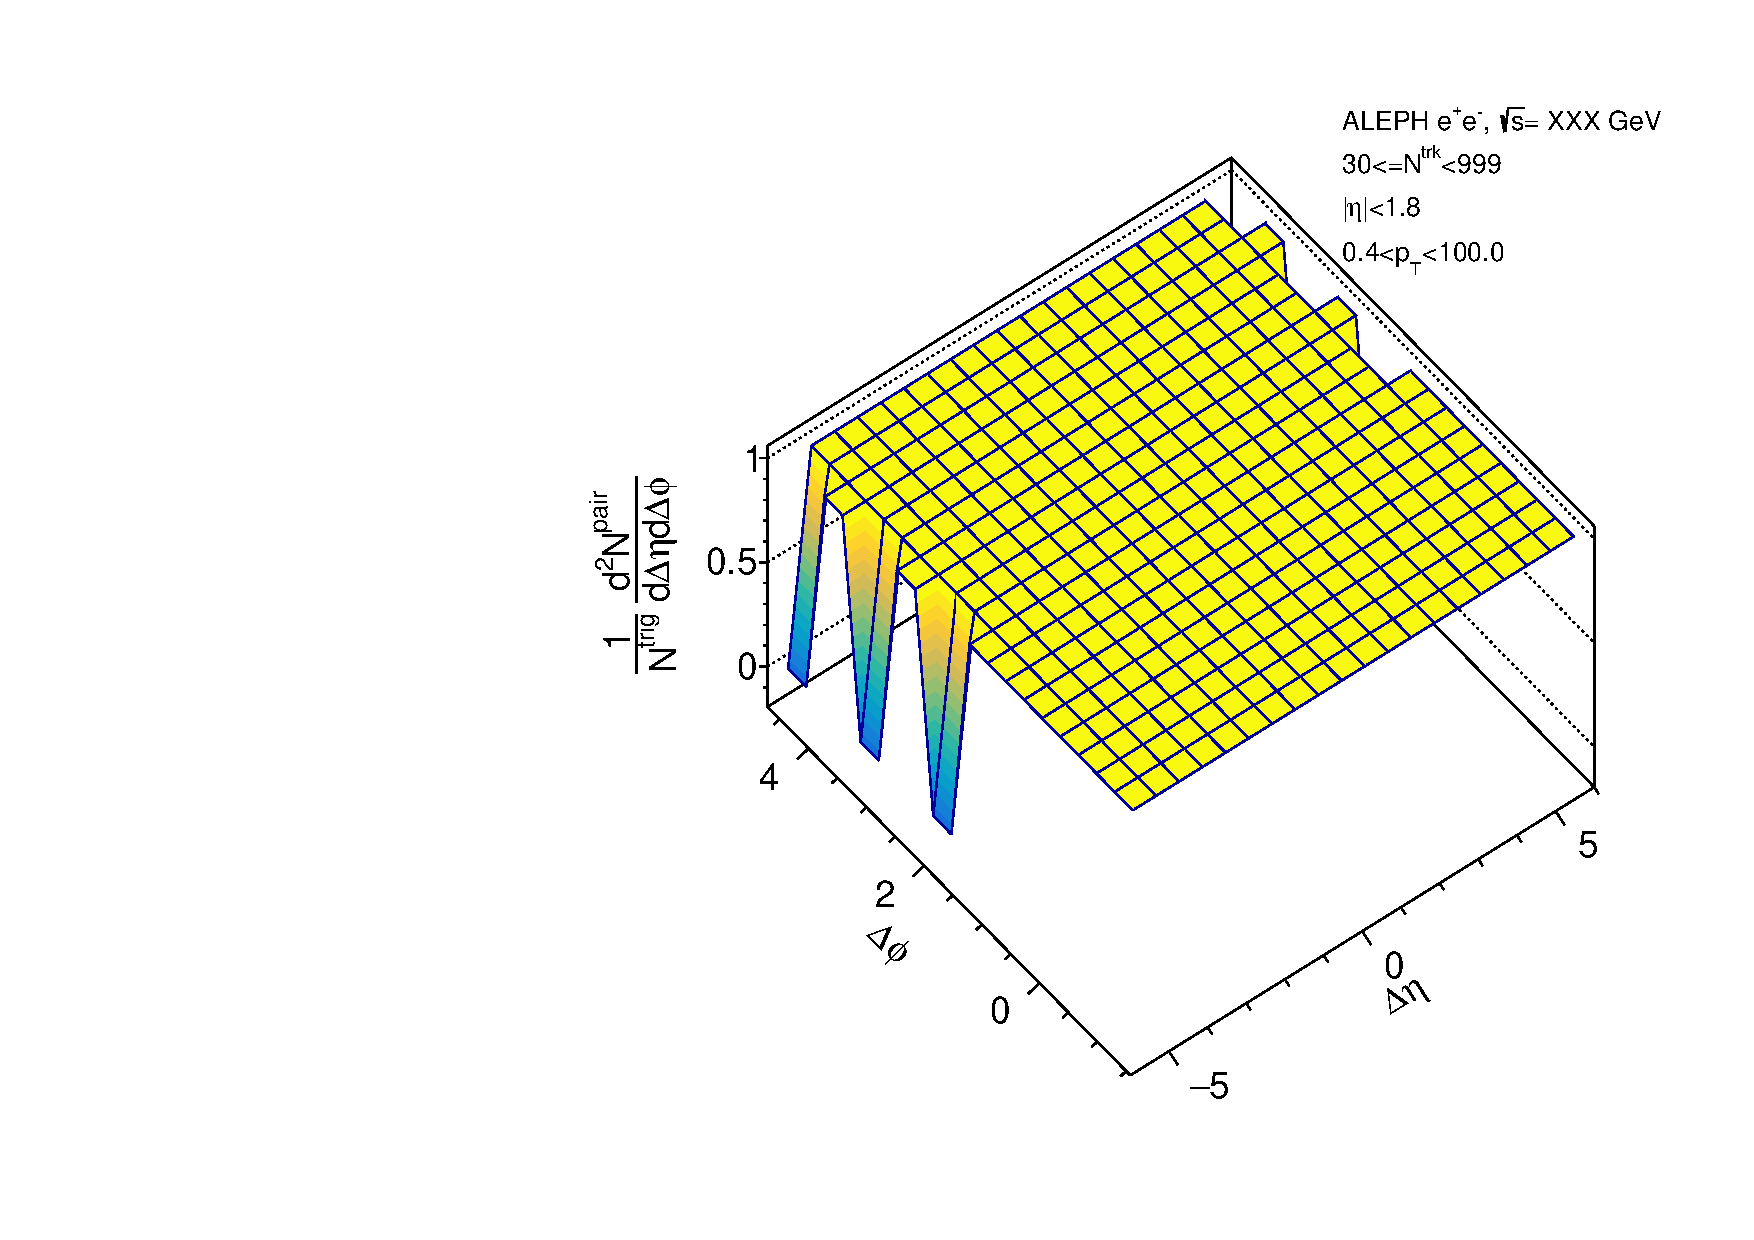
\includegraphics[width=.32\textwidth]{images/TwoParticleCorrelation/CrossCheck/20180126/LEP1_THRUST/LEP1_THRUST_r_ratio_30_999.pdf}} \\
\caption{Two particle correlation fuctions for the LEP1 data set analyzed in the thrust axis.}
\label{fig:test}
\end{figure}

\begin{figure}[H]
\centering
\subfloat{\label{sfig:a}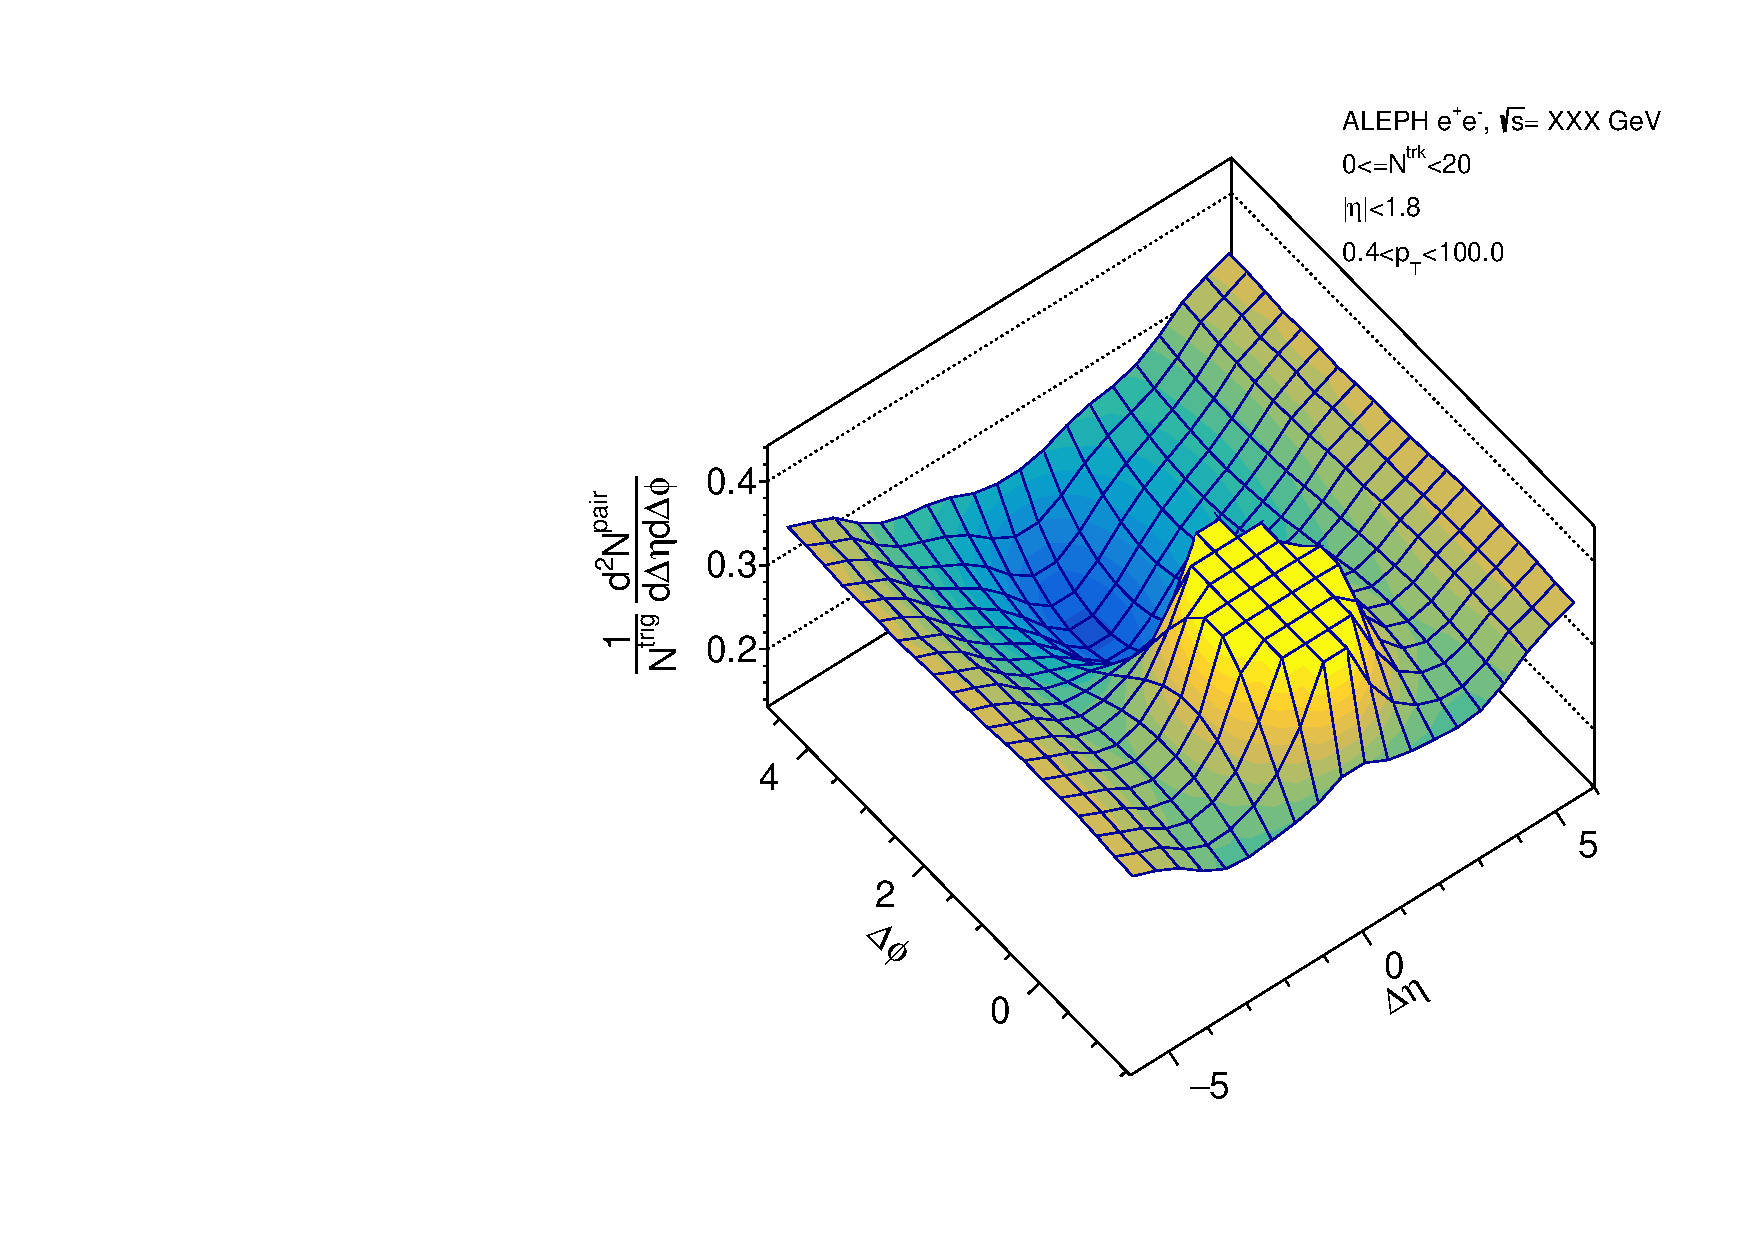
\includegraphics[width=.32\textwidth]{images/TwoParticleCorrelation/CrossCheck/20180126/LEP1_WTA/LEP1_WTA_ratio2_0_20.pdf}}\hfill
\subfloat{\label{sfig:b}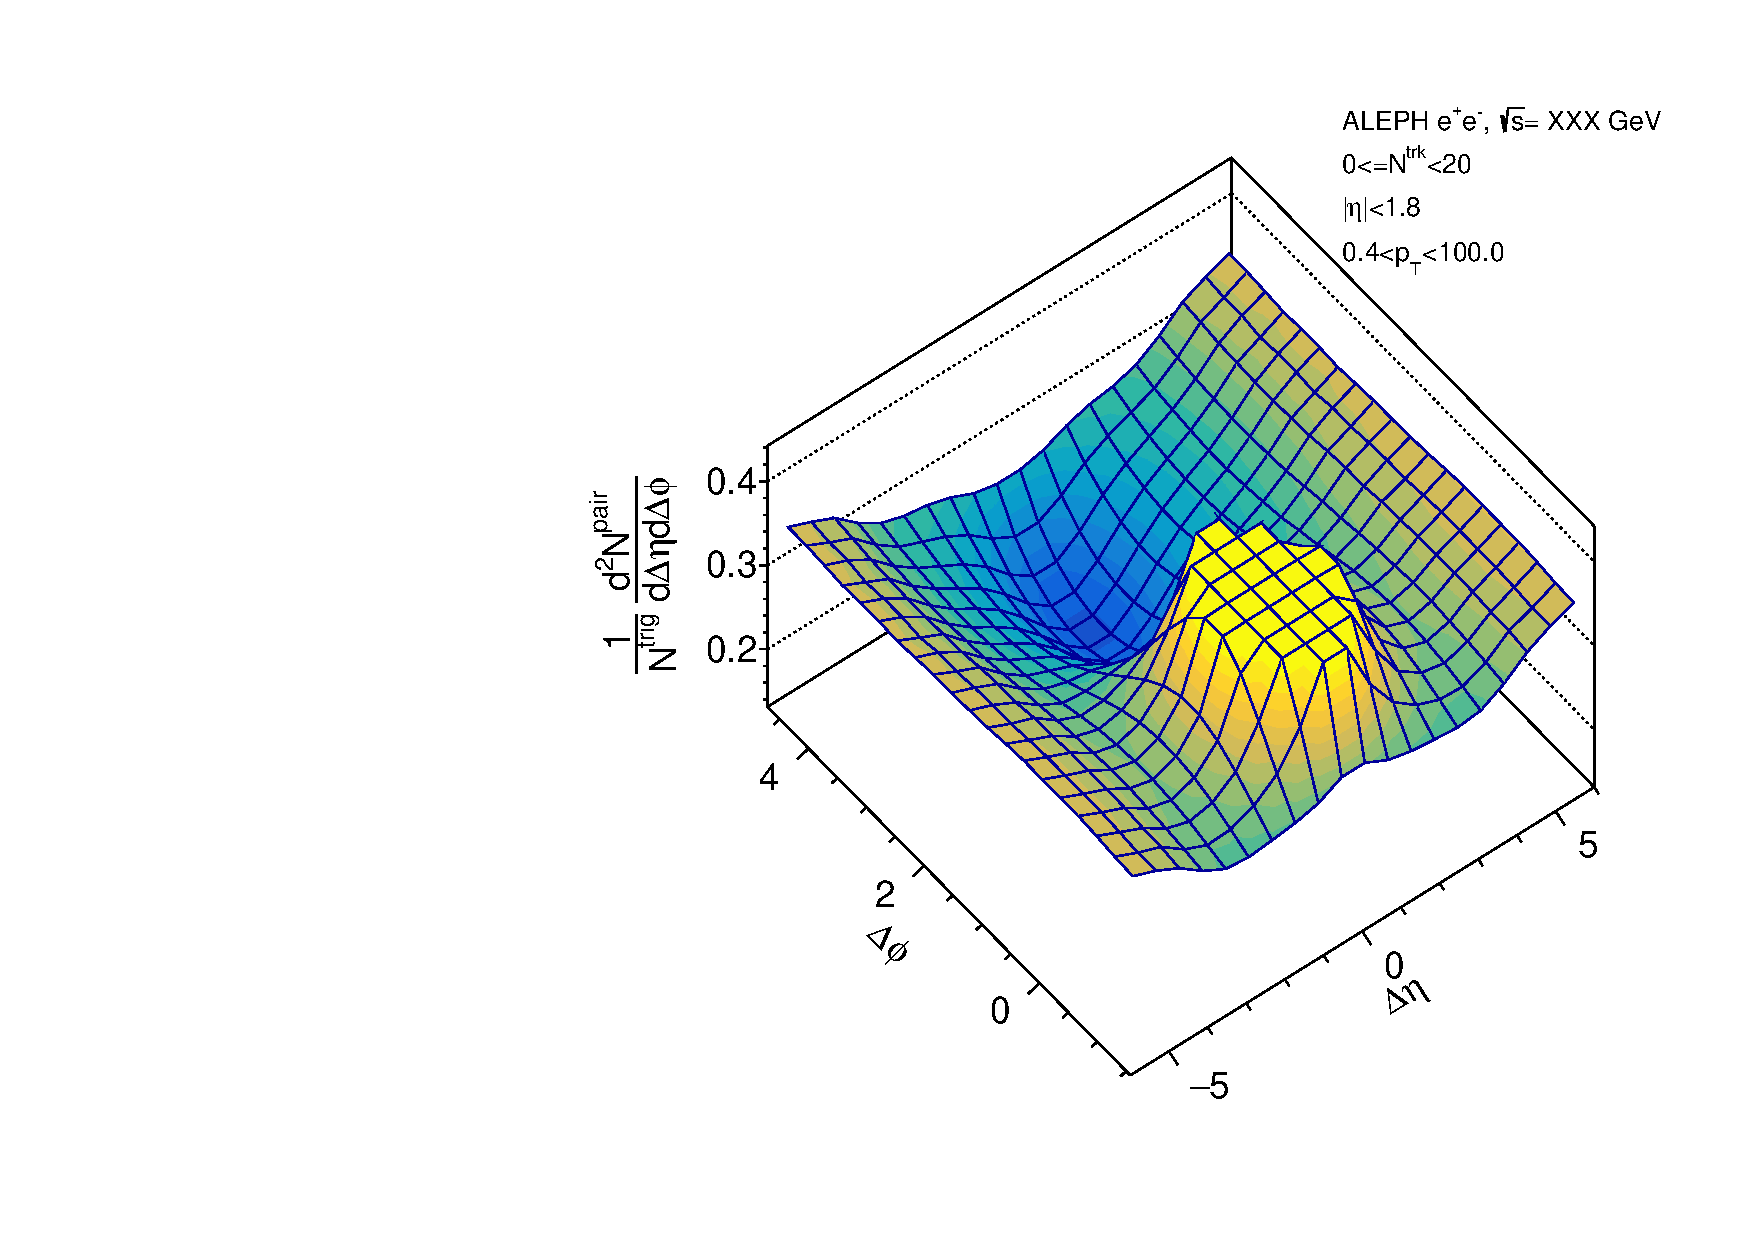
\includegraphics[width=.32\textwidth]{images/TwoParticleCorrelation/CrossCheck/20180126/LEP1_WTA/LEP1_WTA_ratio1_0_20.pdf}}\hfill
\subfloat{\label{sfig:c}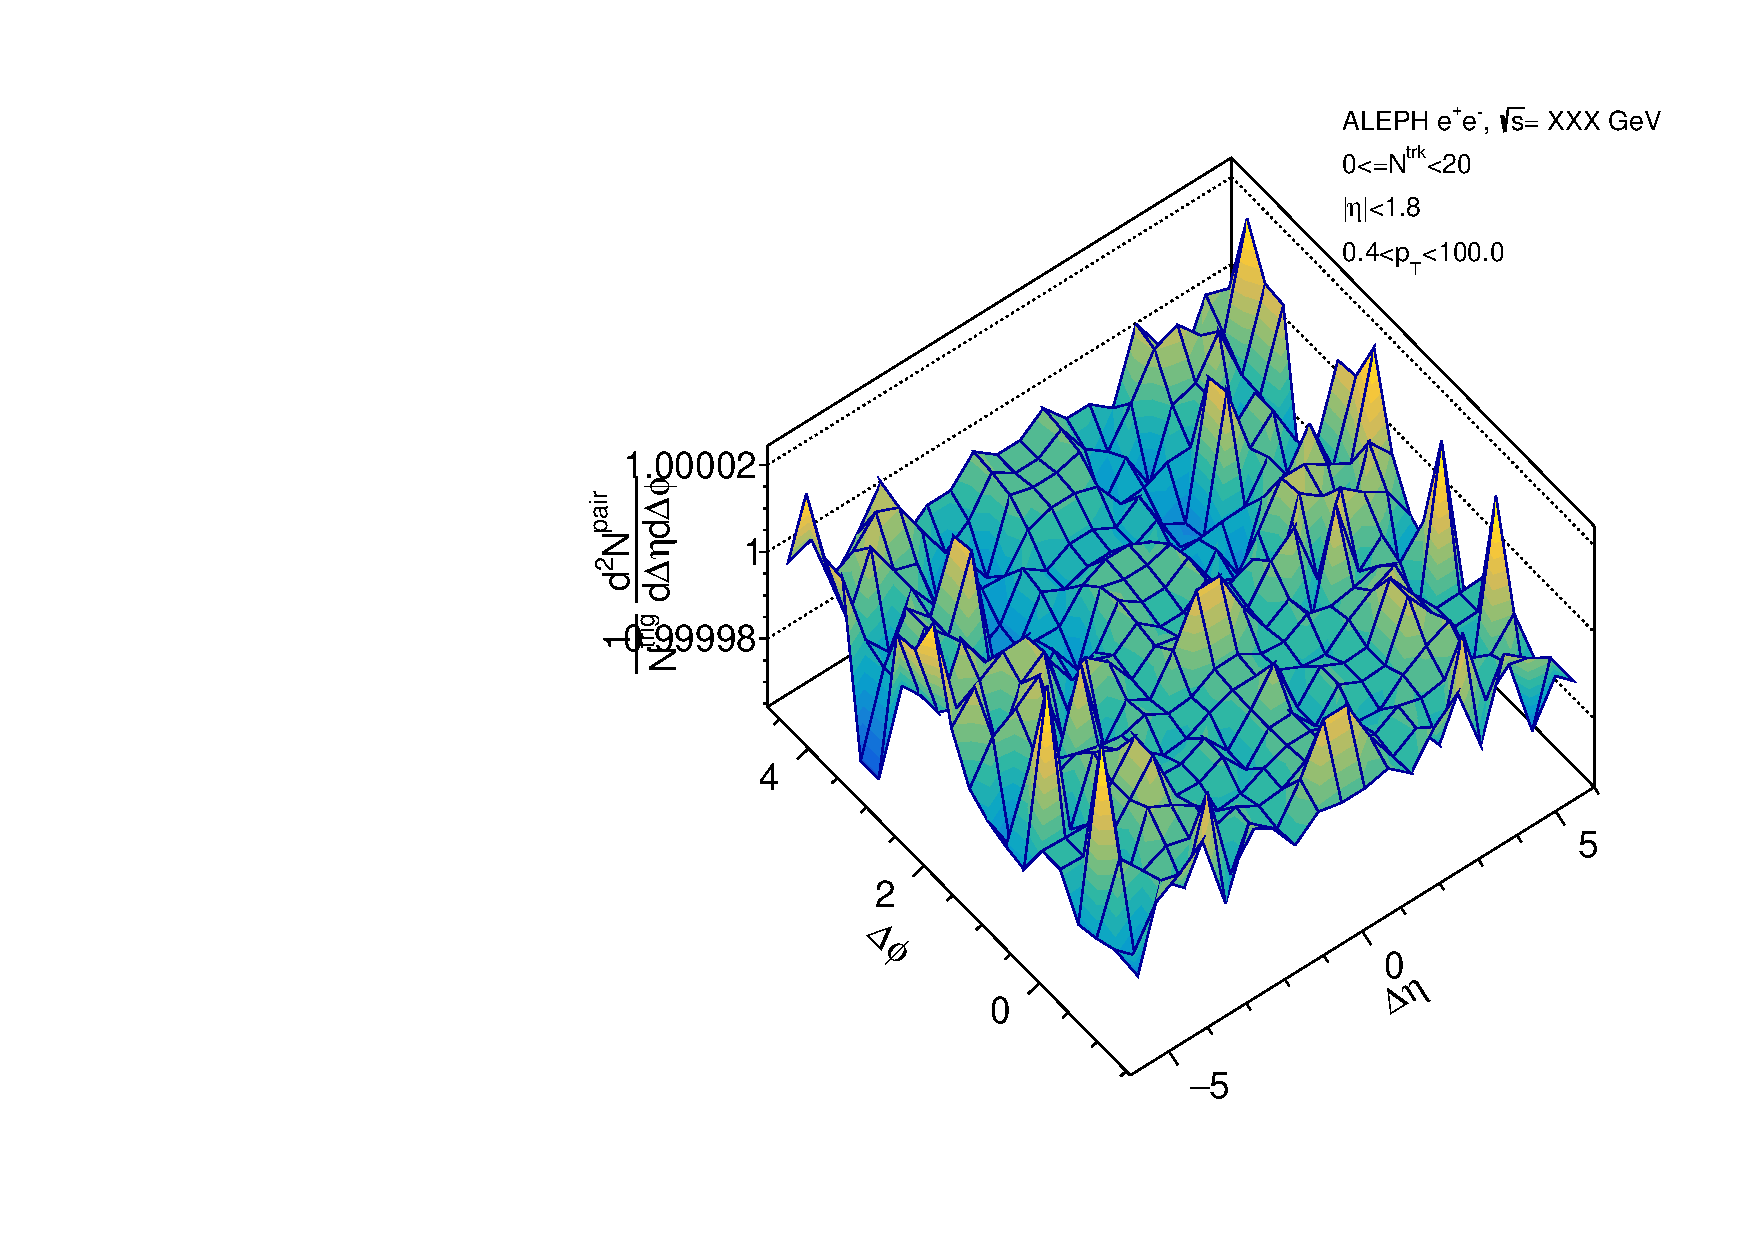
\includegraphics[width=.32\textwidth]{images/TwoParticleCorrelation/CrossCheck/20180126/LEP1_WTA/LEP1_WTA_r_ratio_0_20.pdf}}\hfill
\subfloat{\label{sfig:d}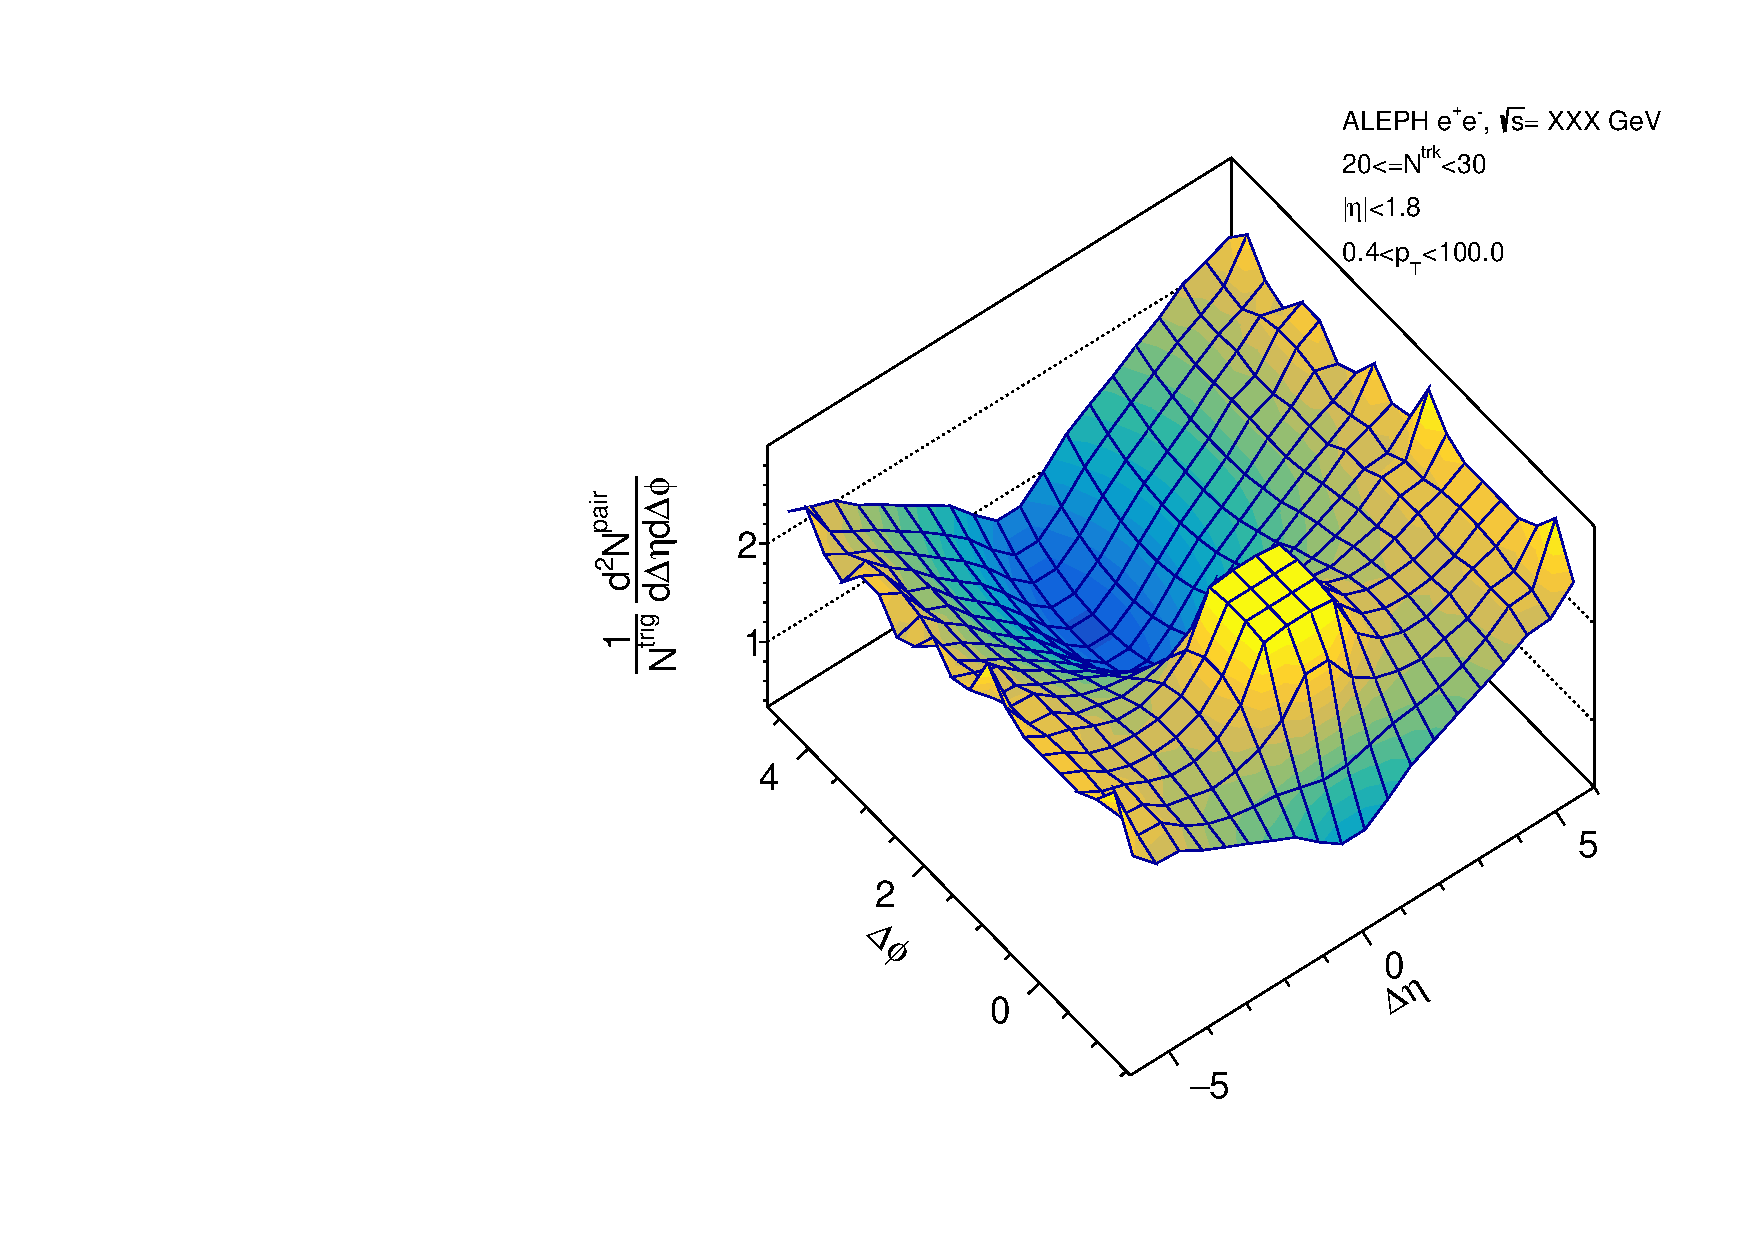
\includegraphics[width=.32\textwidth]{images/TwoParticleCorrelation/CrossCheck/20180126/LEP1_WTA/LEP1_WTA_ratio2_20_30.pdf}}\hfill
\subfloat{\label{sfig:e}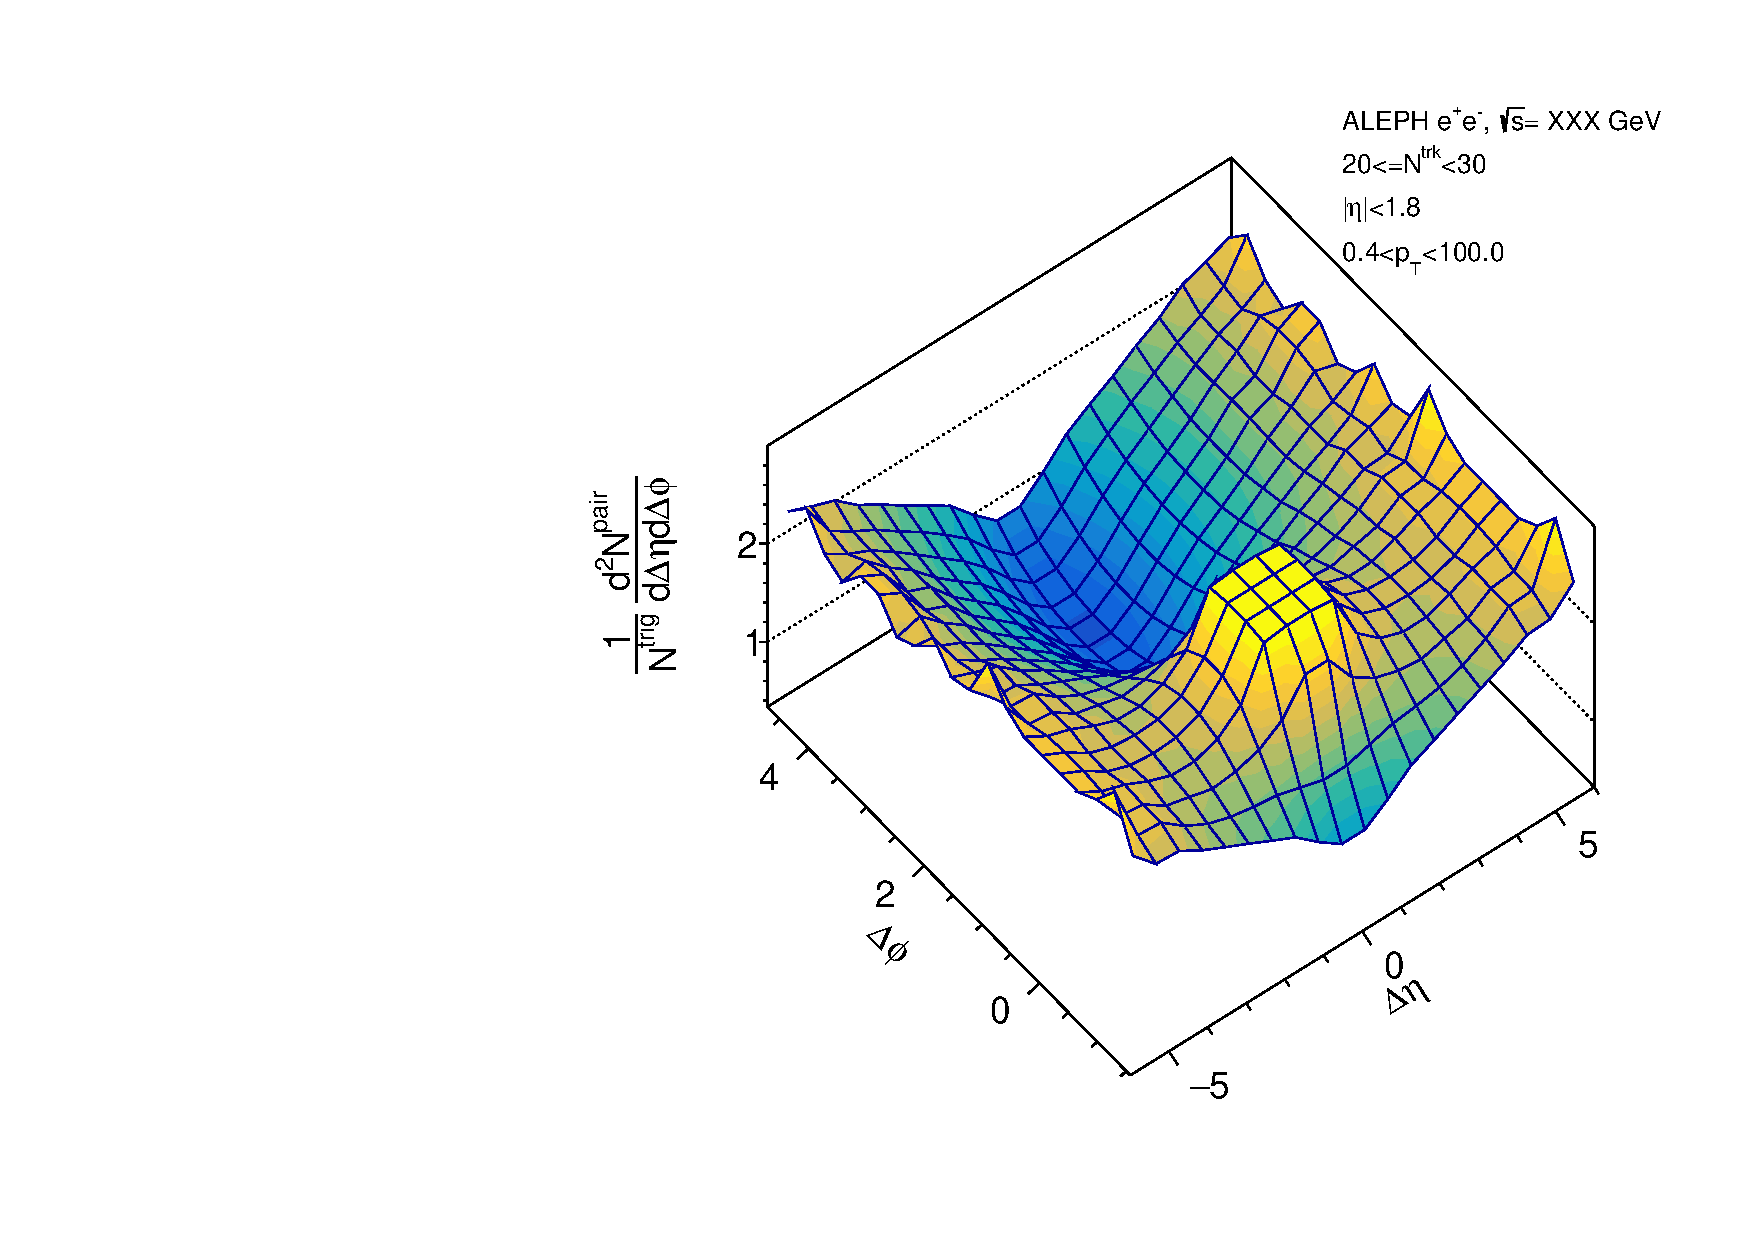
\includegraphics[width=.32\textwidth]{images/TwoParticleCorrelation/CrossCheck/20180126/LEP1_WTA/LEP1_WTA_ratio1_20_30.pdf}}\hfill
\subfloat{\label{sfig:f}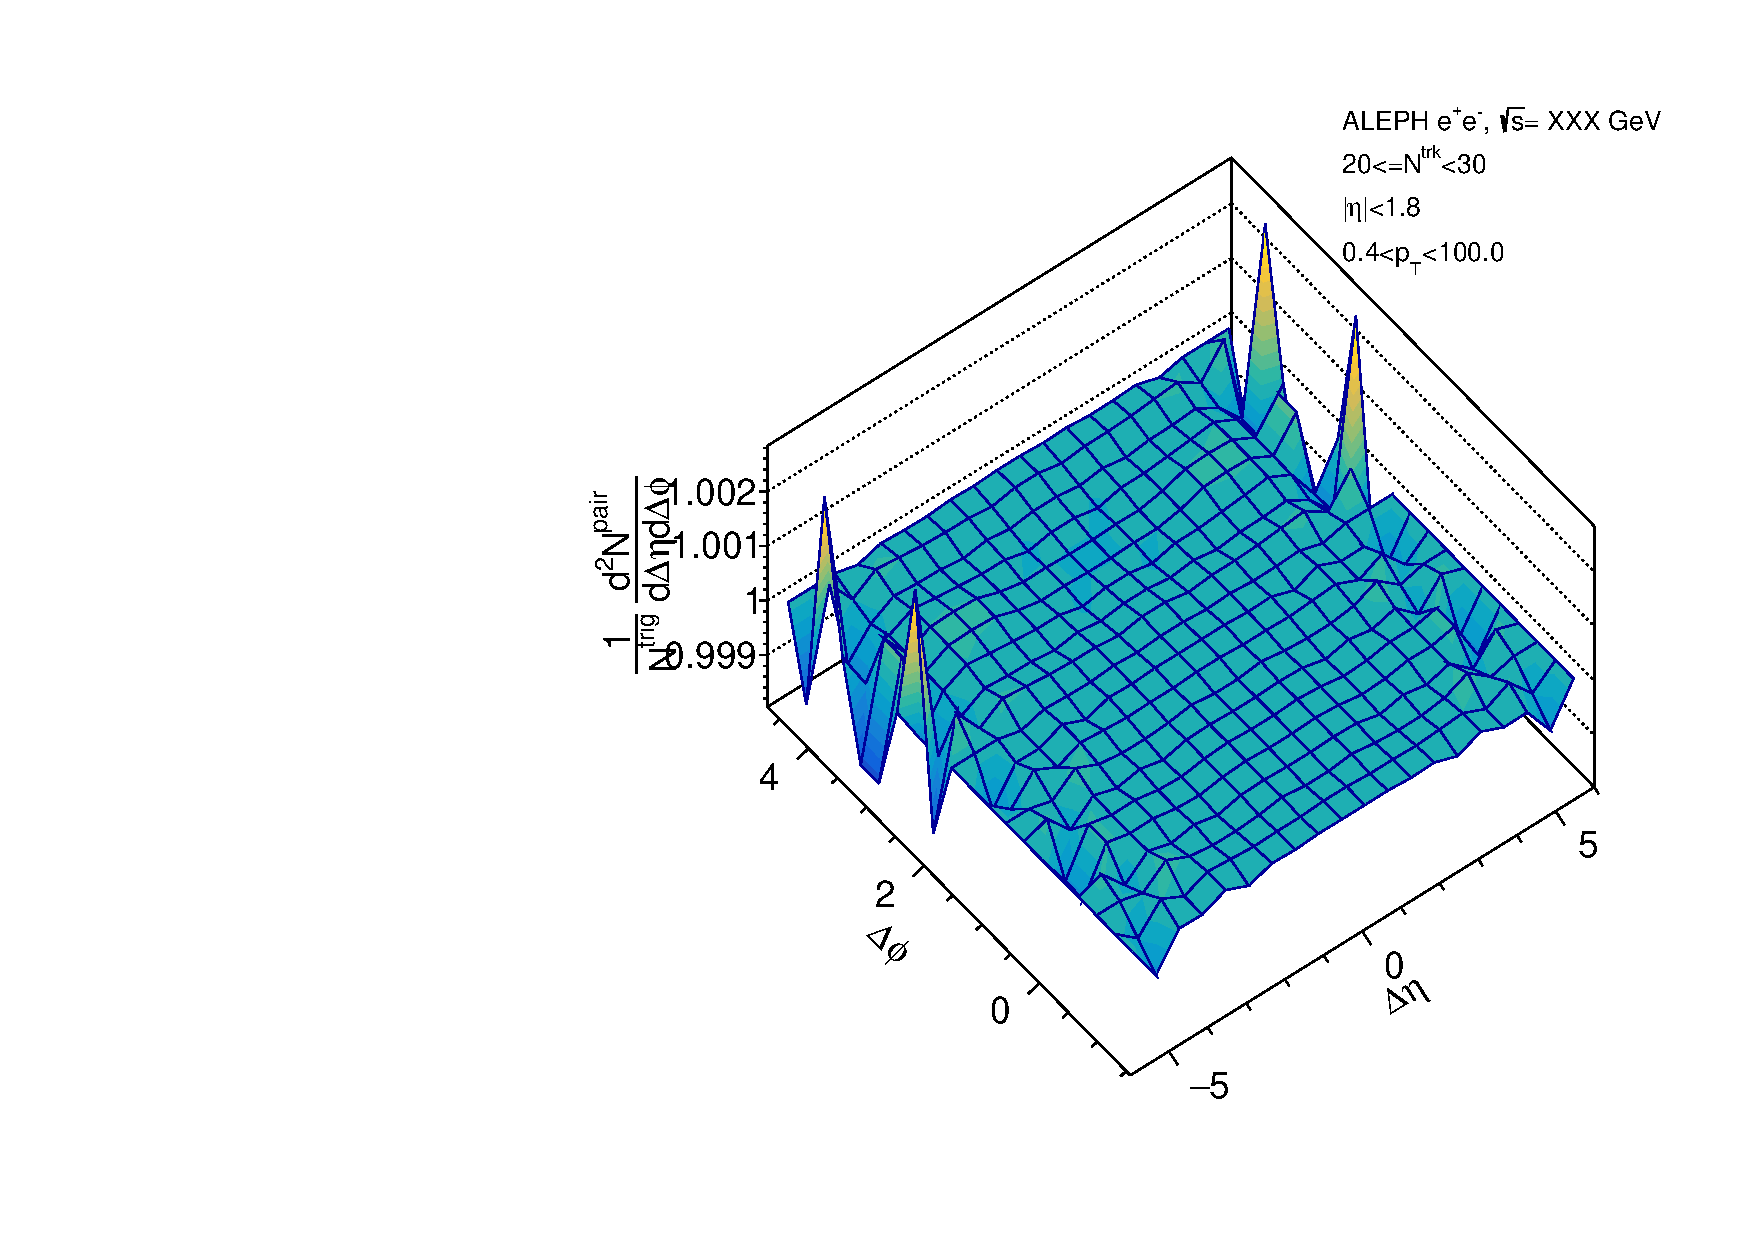
\includegraphics[width=.32\textwidth]{images/TwoParticleCorrelation/CrossCheck/20180126/LEP1_WTA/LEP1_WTA_r_ratio_20_30.pdf}}\hfill
\subfloat{\label{sfig:g}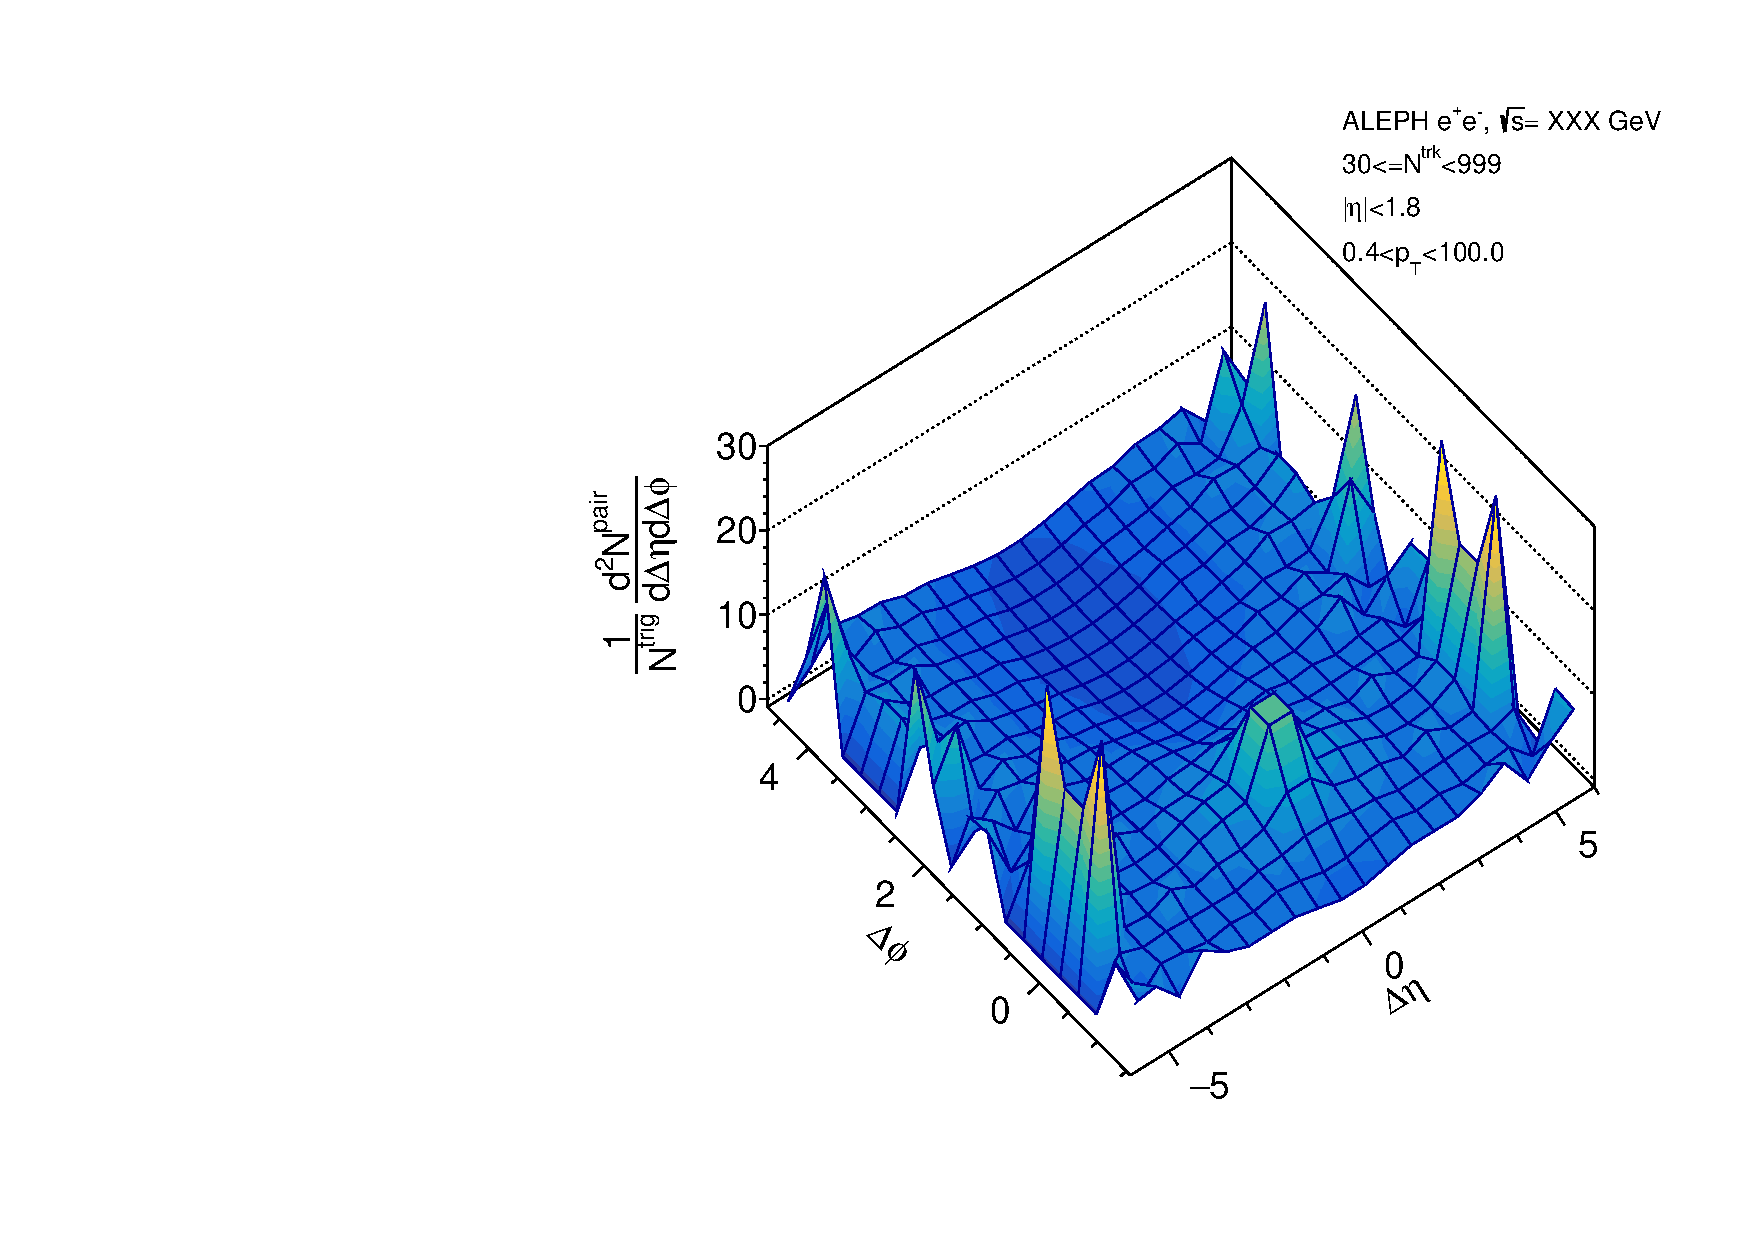
\includegraphics[width=.32\textwidth]{images/TwoParticleCorrelation/CrossCheck/20180126/LEP1_WTA/LEP1_WTA_ratio2_30_999.pdf}}\hfill
\subfloat{\label{sfig:h}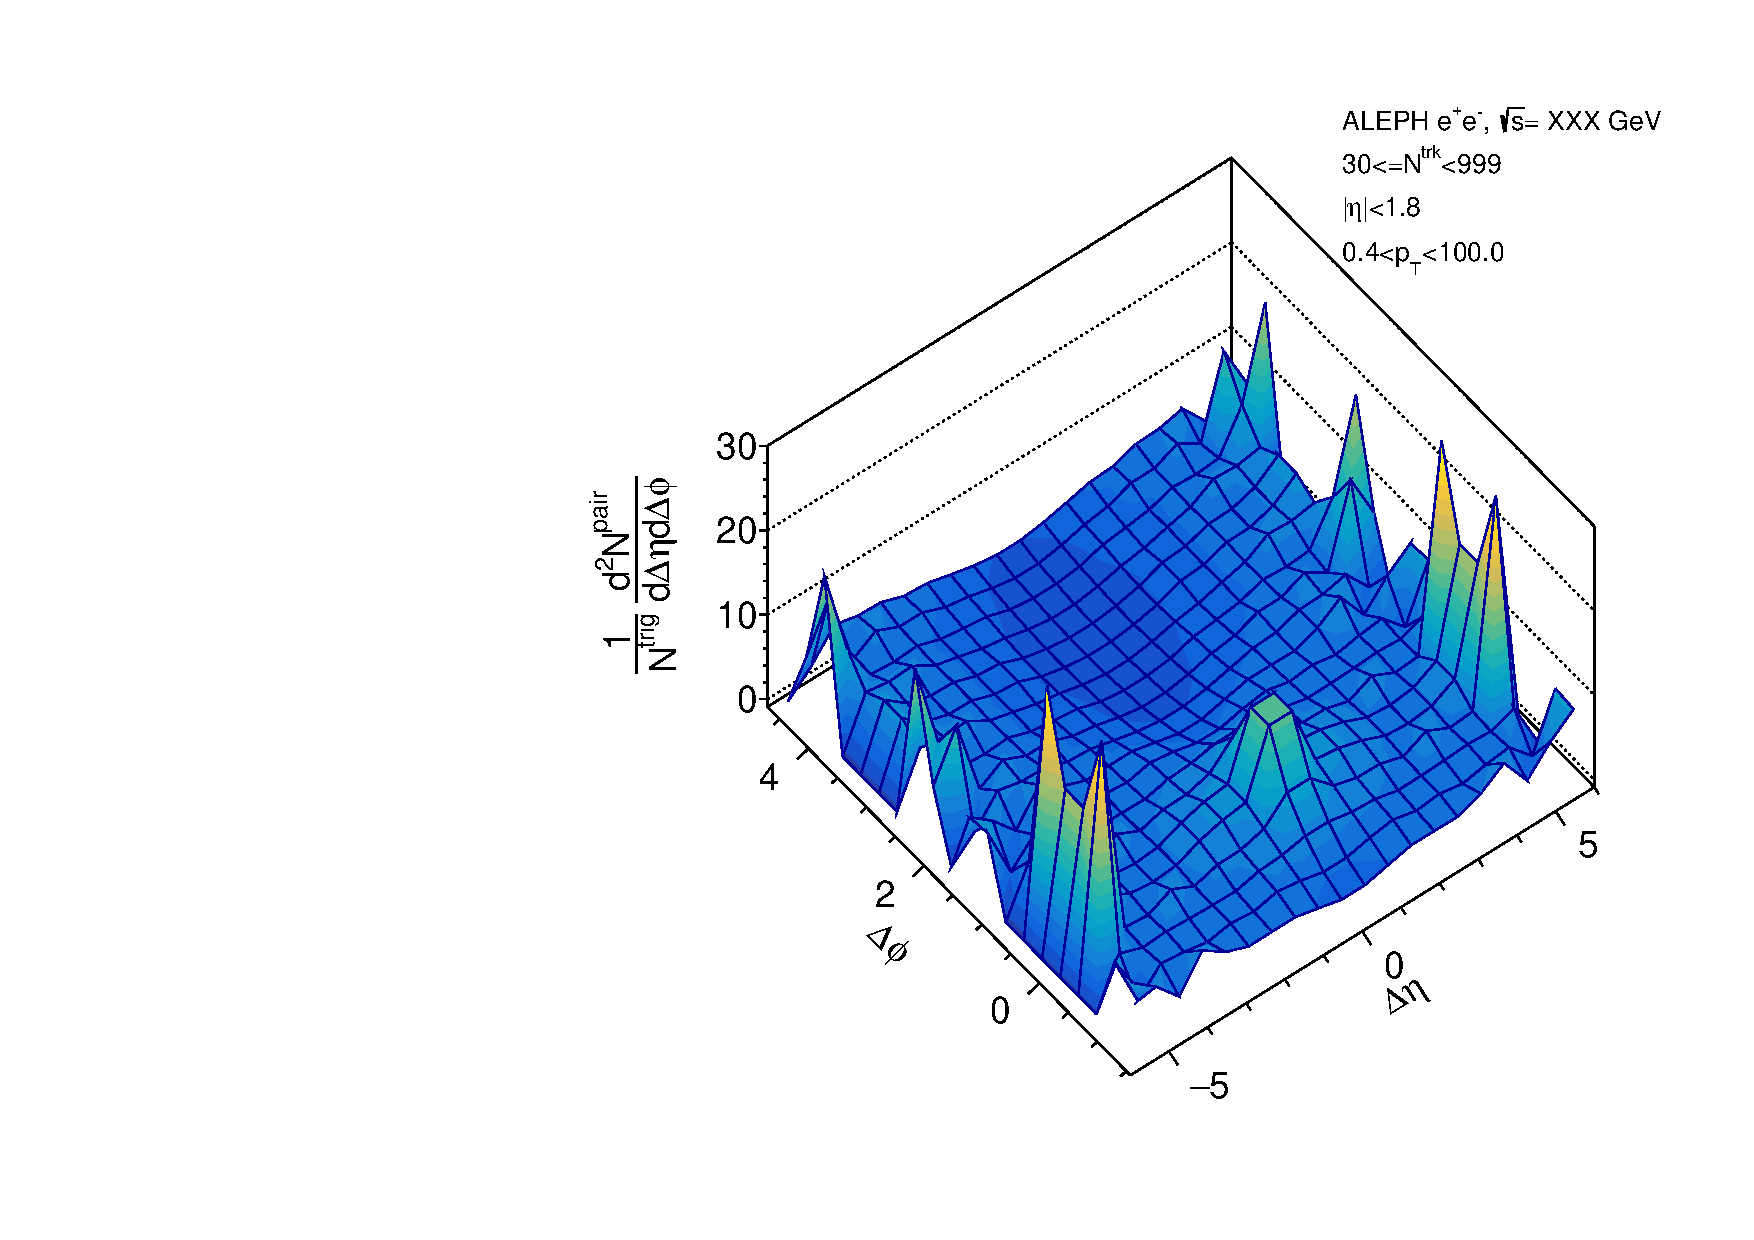
\includegraphics[width=.32\textwidth]{images/TwoParticleCorrelation/CrossCheck/20180126/LEP1_WTA/LEP1_WTA_ratio1_30_999.pdf}}\hfill
\subfloat{\label{sfig:i}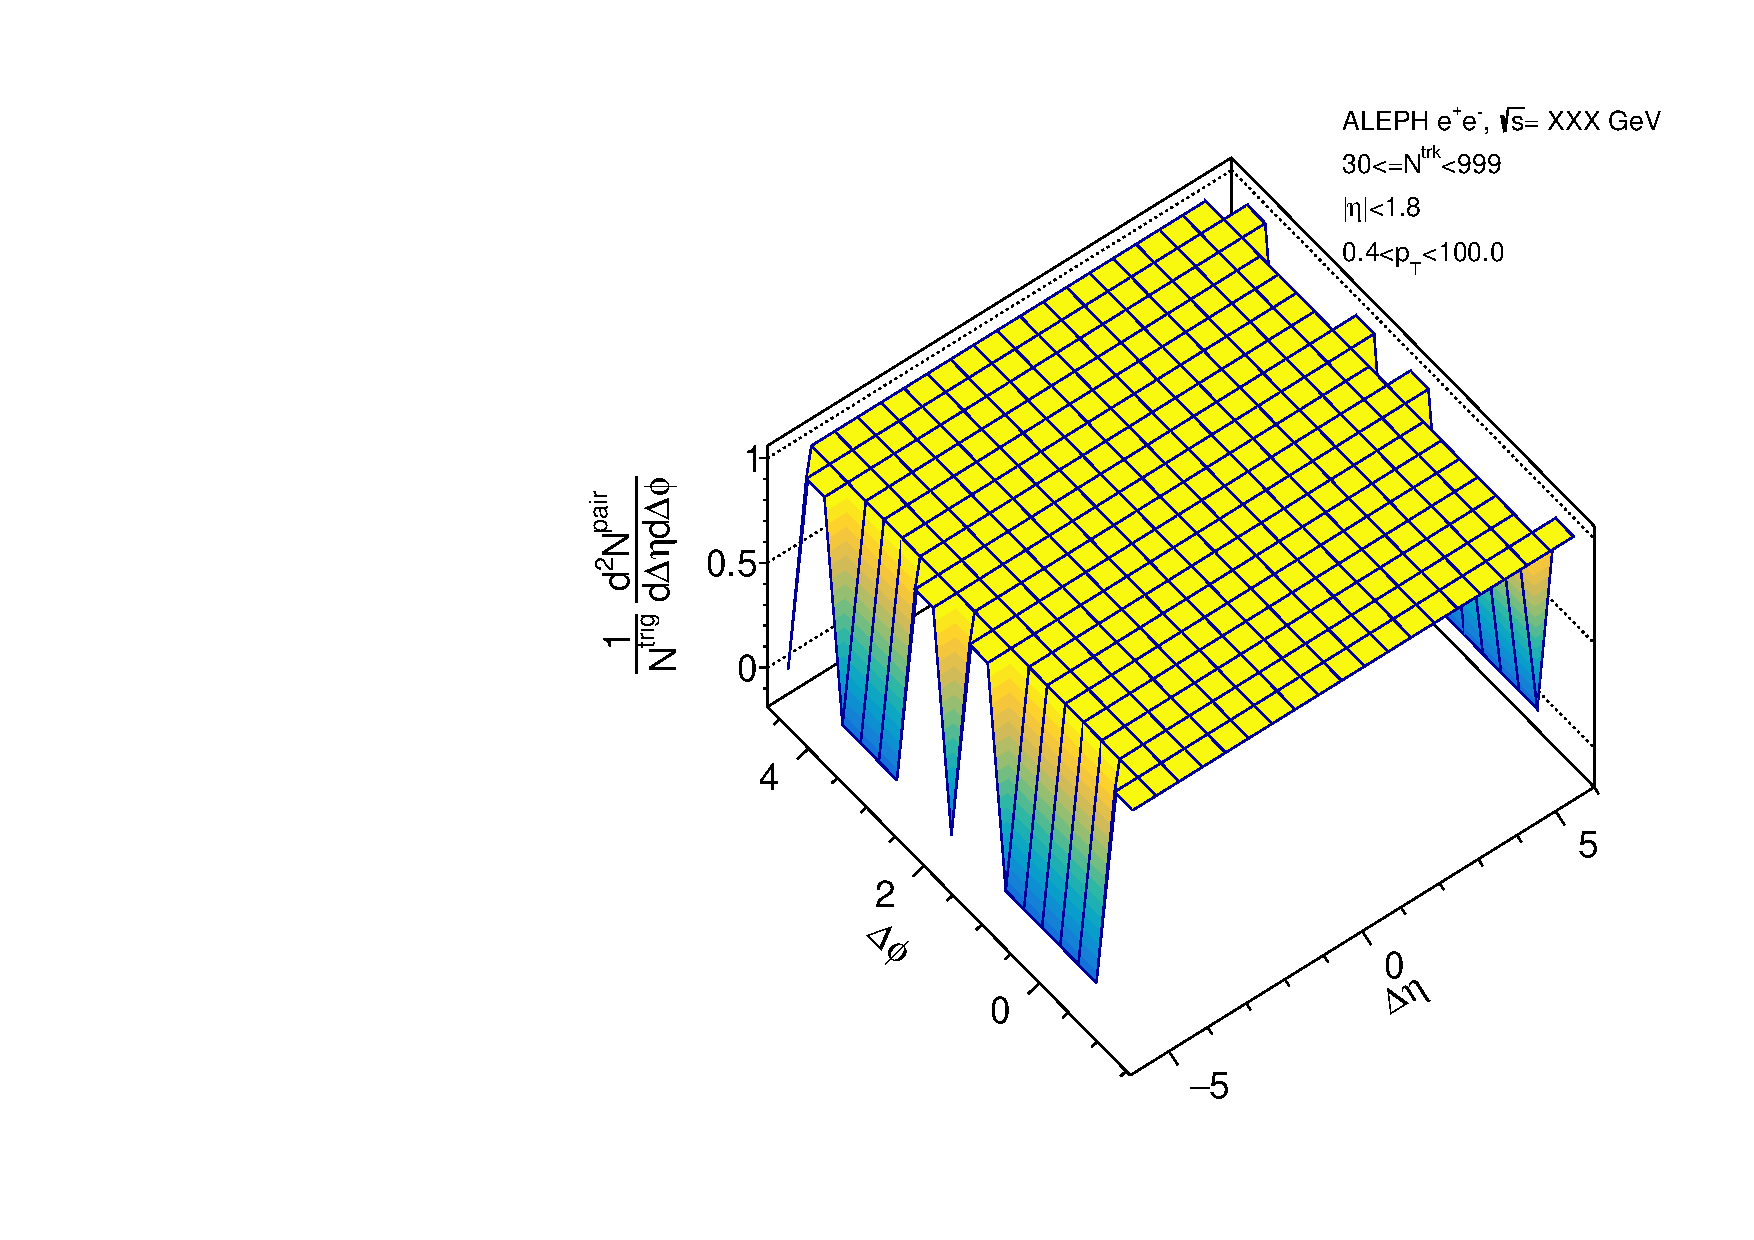
\includegraphics[width=.32\textwidth]{images/TwoParticleCorrelation/CrossCheck/20180126/LEP1_WTA/LEP1_WTA_r_ratio_30_999.pdf}} \\
\caption{Two particle correlation fuctions for the LEP1 data set analyzed in the WTA axis.}
\label{fig:test}
\end{figure}

%%%%%%%%%%% LEP2 %%%%%%%%%%%
\begin{figure}[H]
\centering
\subfloat{\label{sfig:a}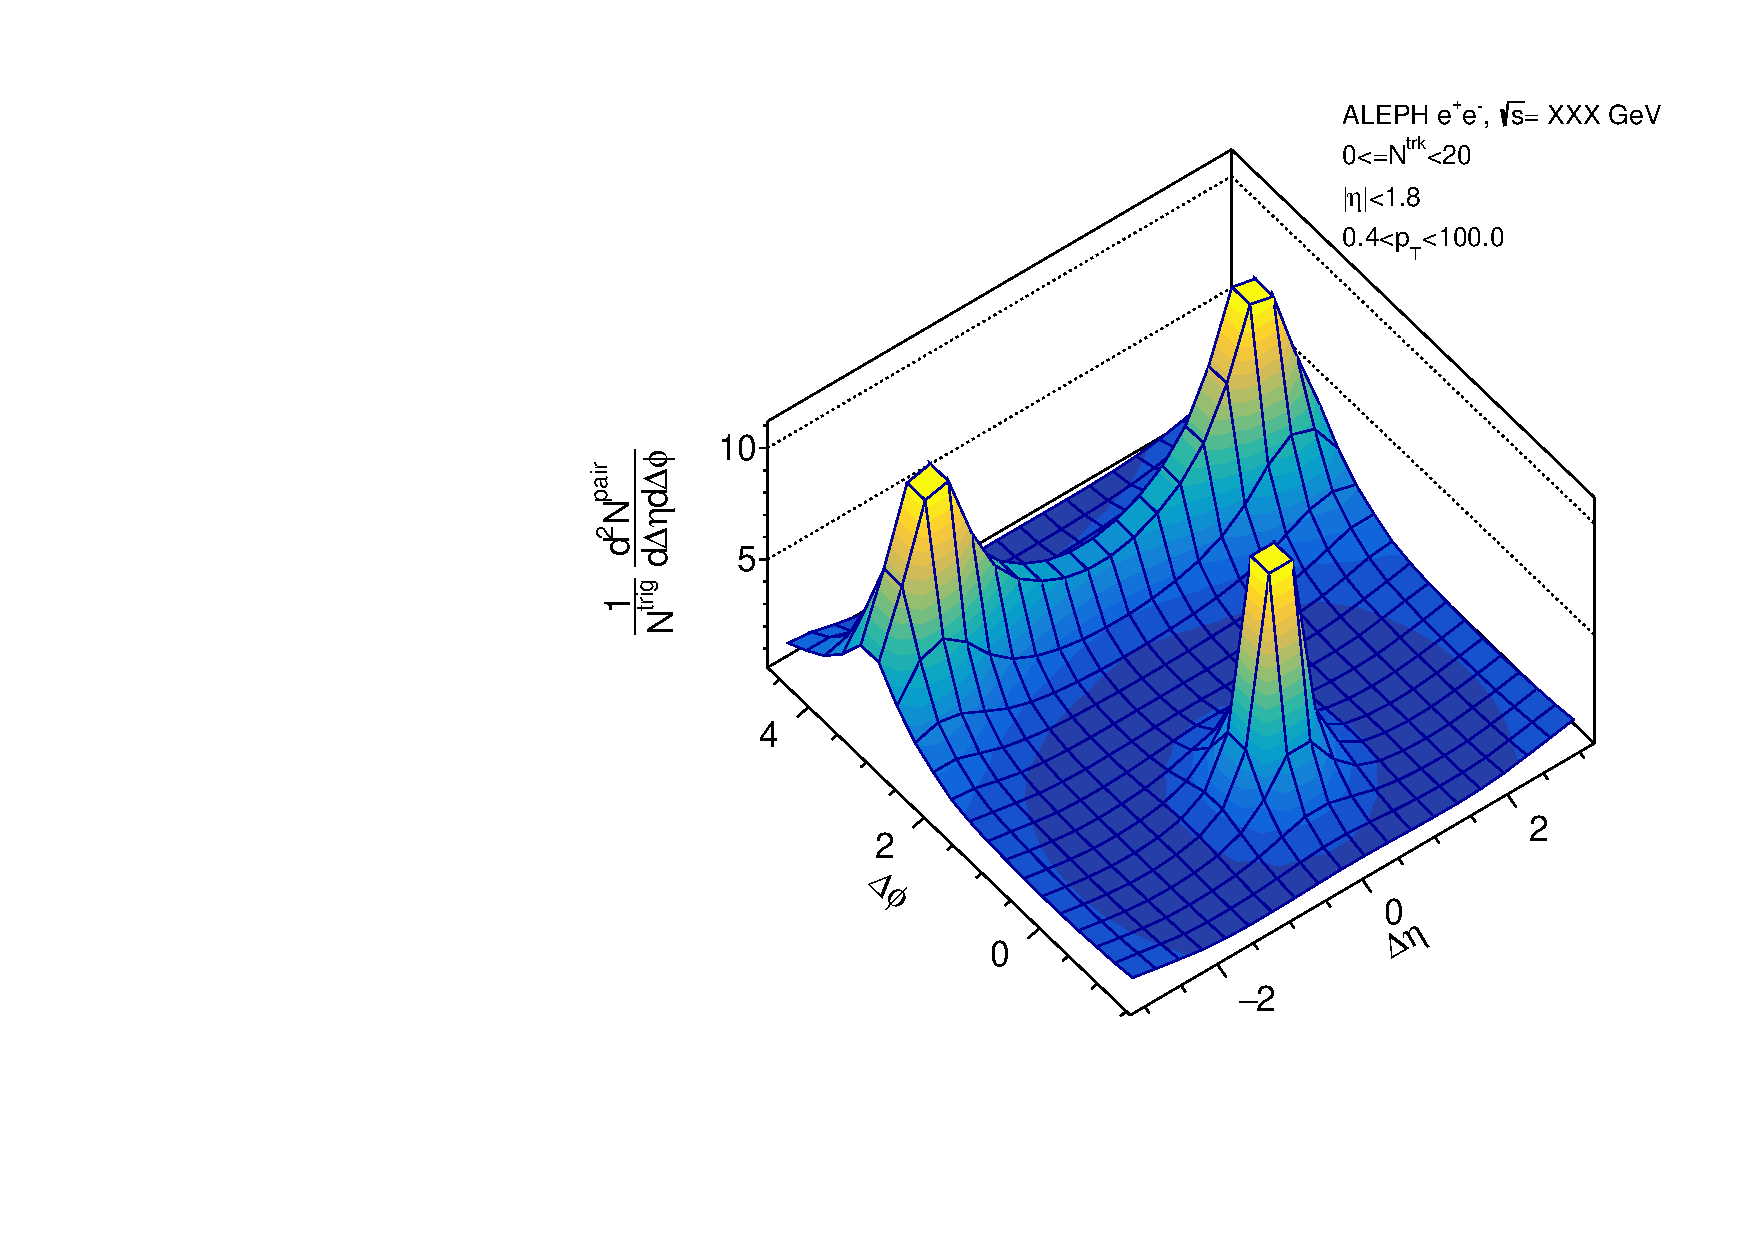
\includegraphics[width=.32\textwidth]{images/TwoParticleCorrelation/CrossCheck/20180126/LEP2_BEAM/LEP2_BEAM_ratio2_0_20.pdf}}\hfill
\subfloat{\label{sfig:b}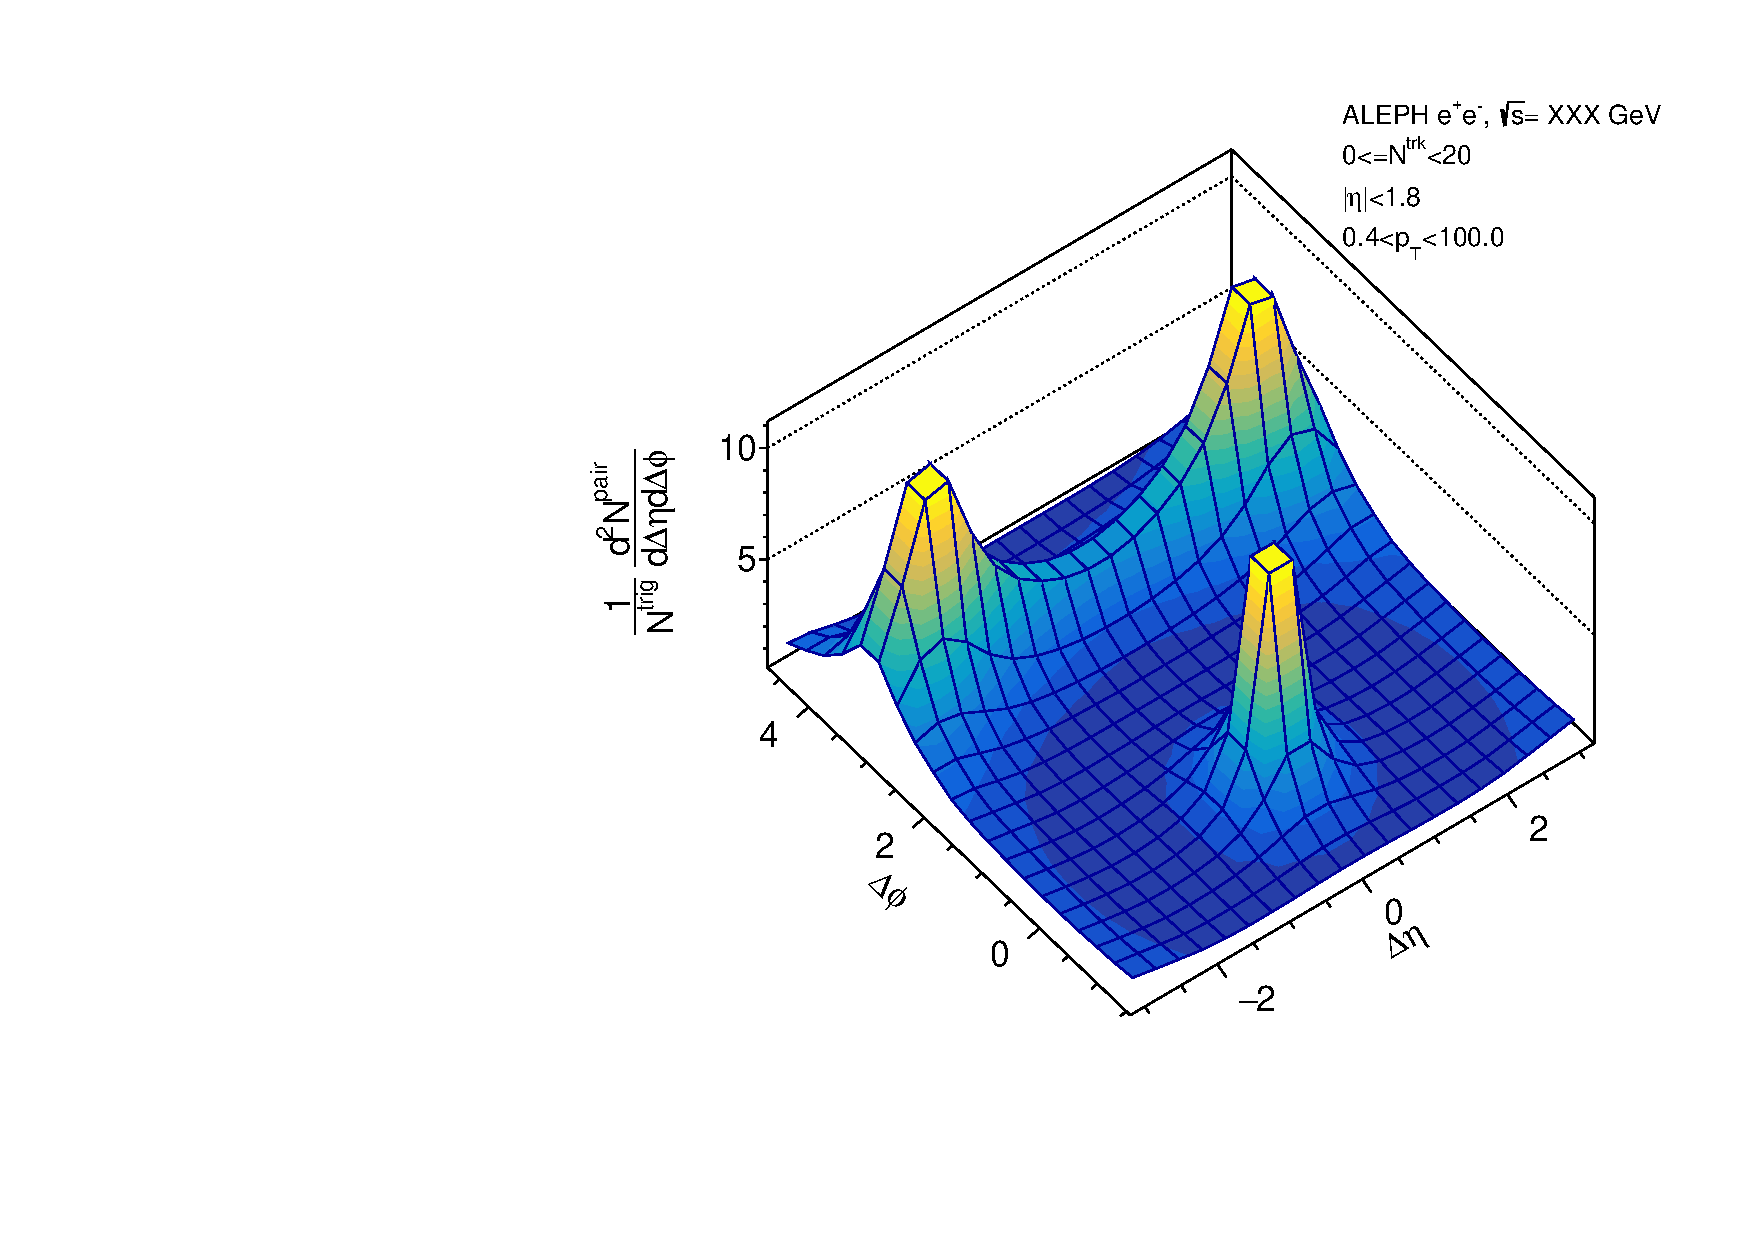
\includegraphics[width=.32\textwidth]{images/TwoParticleCorrelation/CrossCheck/20180126/LEP2_BEAM/LEP2_BEAM_ratio1_0_20.pdf}}\hfill
\subfloat{\label{sfig:c}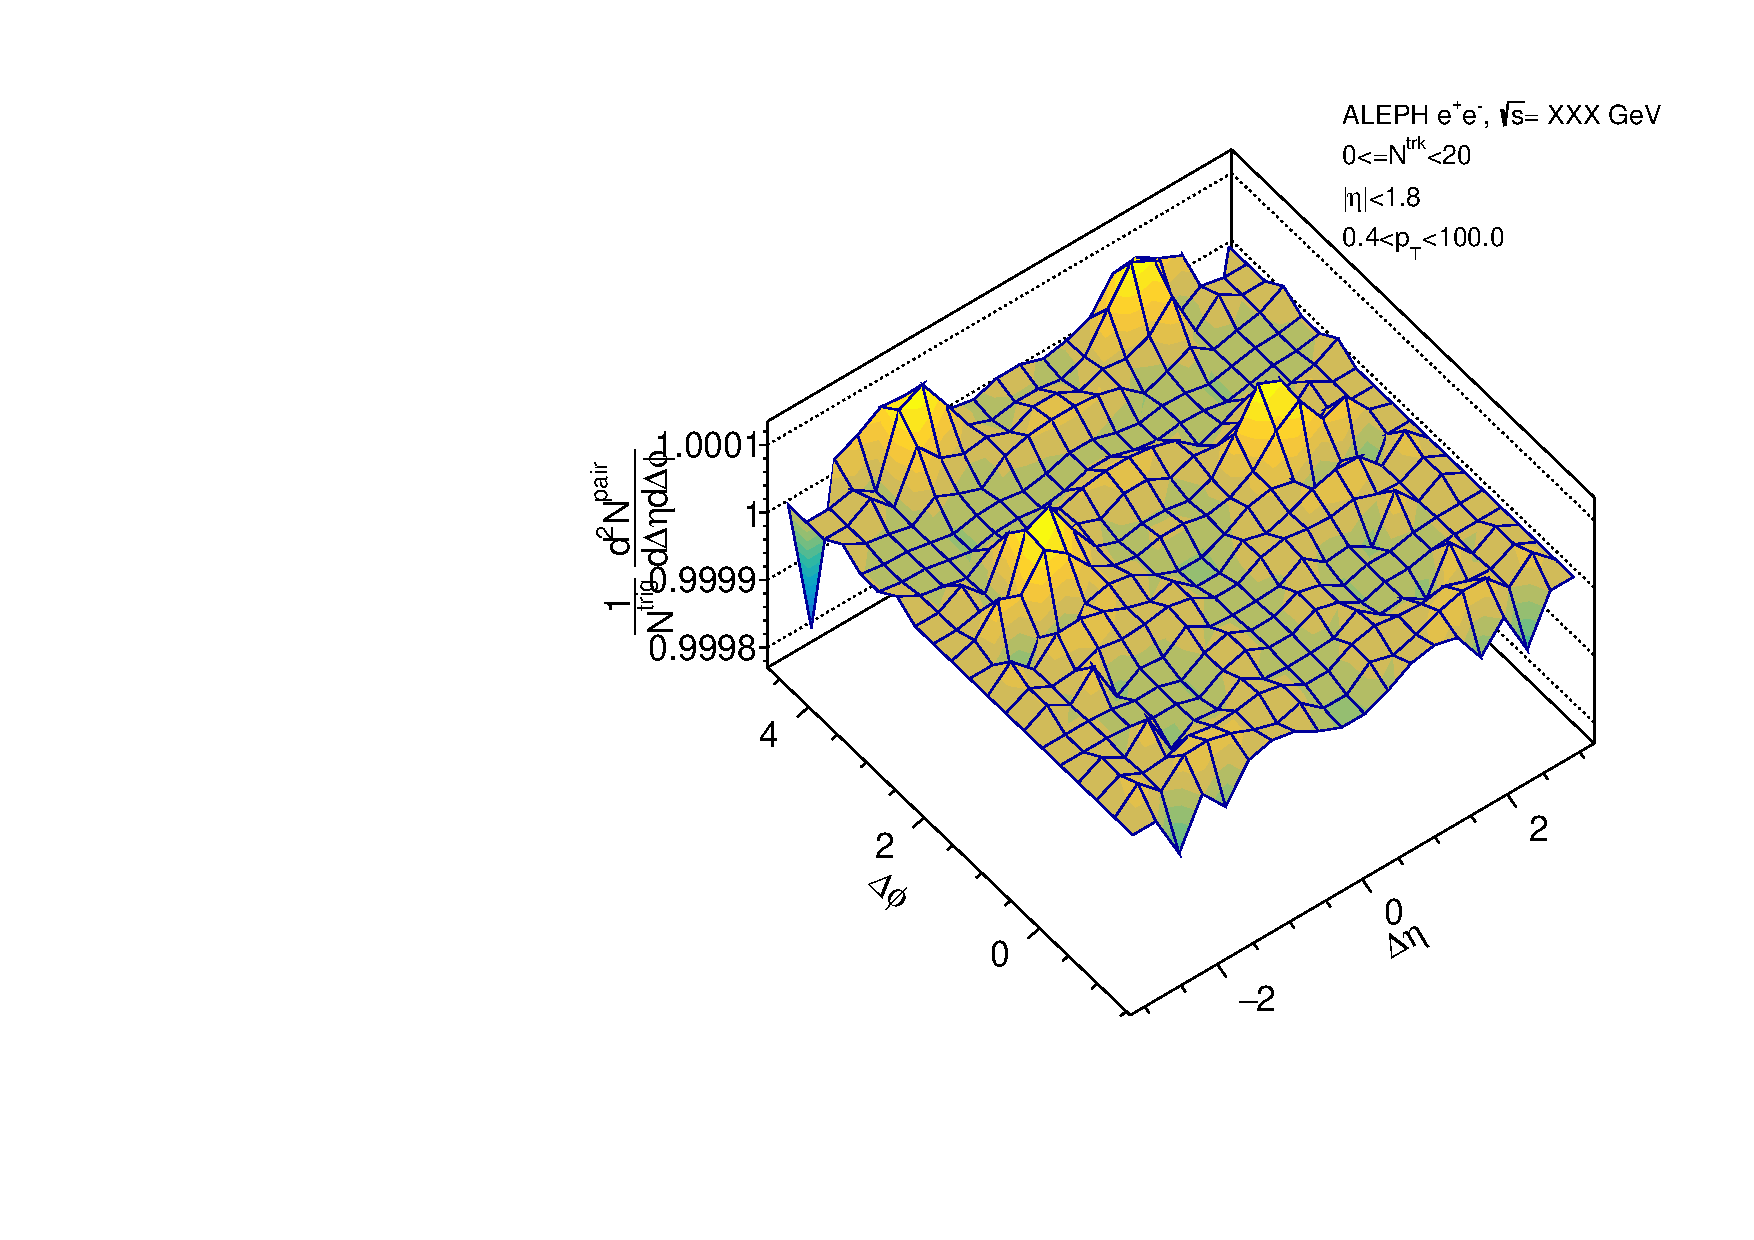
\includegraphics[width=.32\textwidth]{images/TwoParticleCorrelation/CrossCheck/20180126/LEP2_BEAM/LEP2_BEAM_r_ratio_0_20.pdf}}\hfill
\subfloat{\label{sfig:d}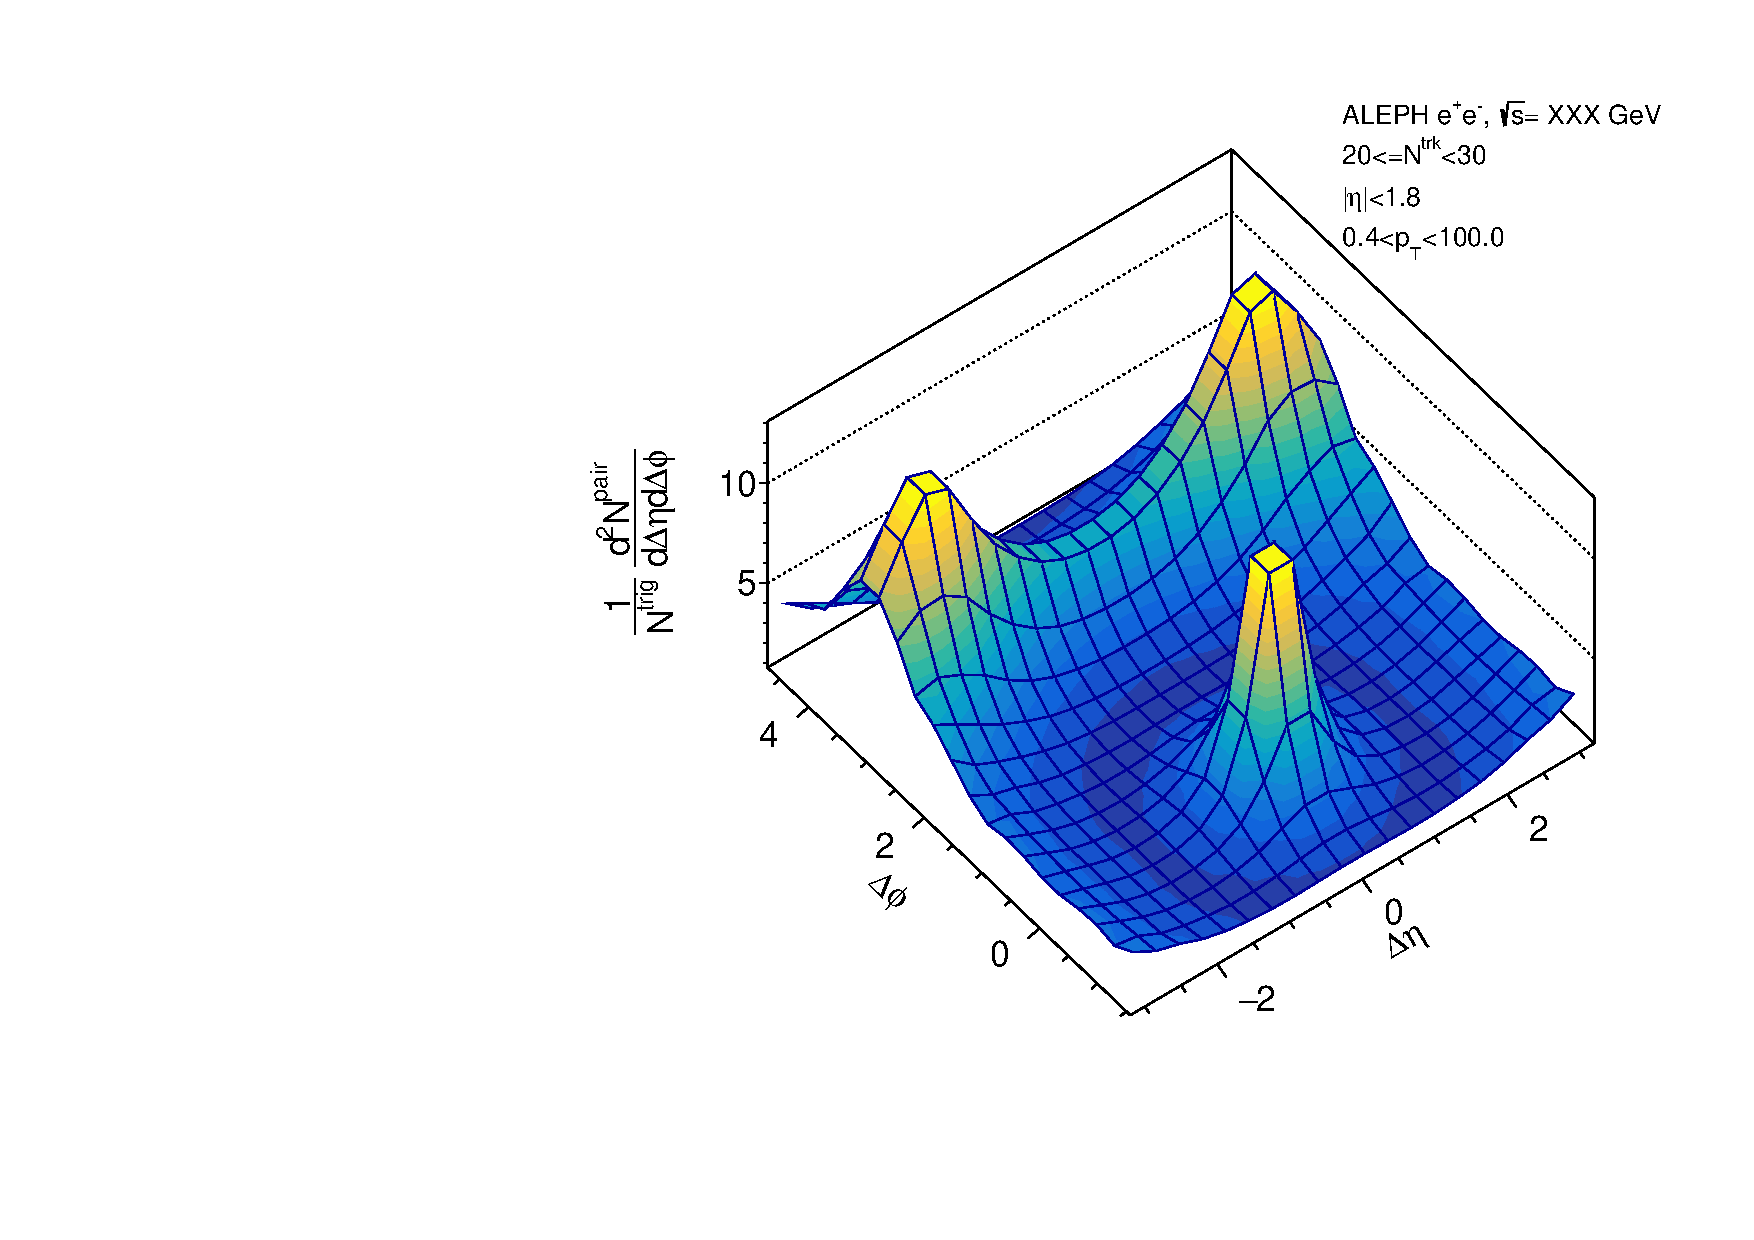
\includegraphics[width=.32\textwidth]{images/TwoParticleCorrelation/CrossCheck/20180126/LEP2_BEAM/LEP2_BEAM_ratio2_20_30.pdf}}\hfill
\subfloat{\label{sfig:e}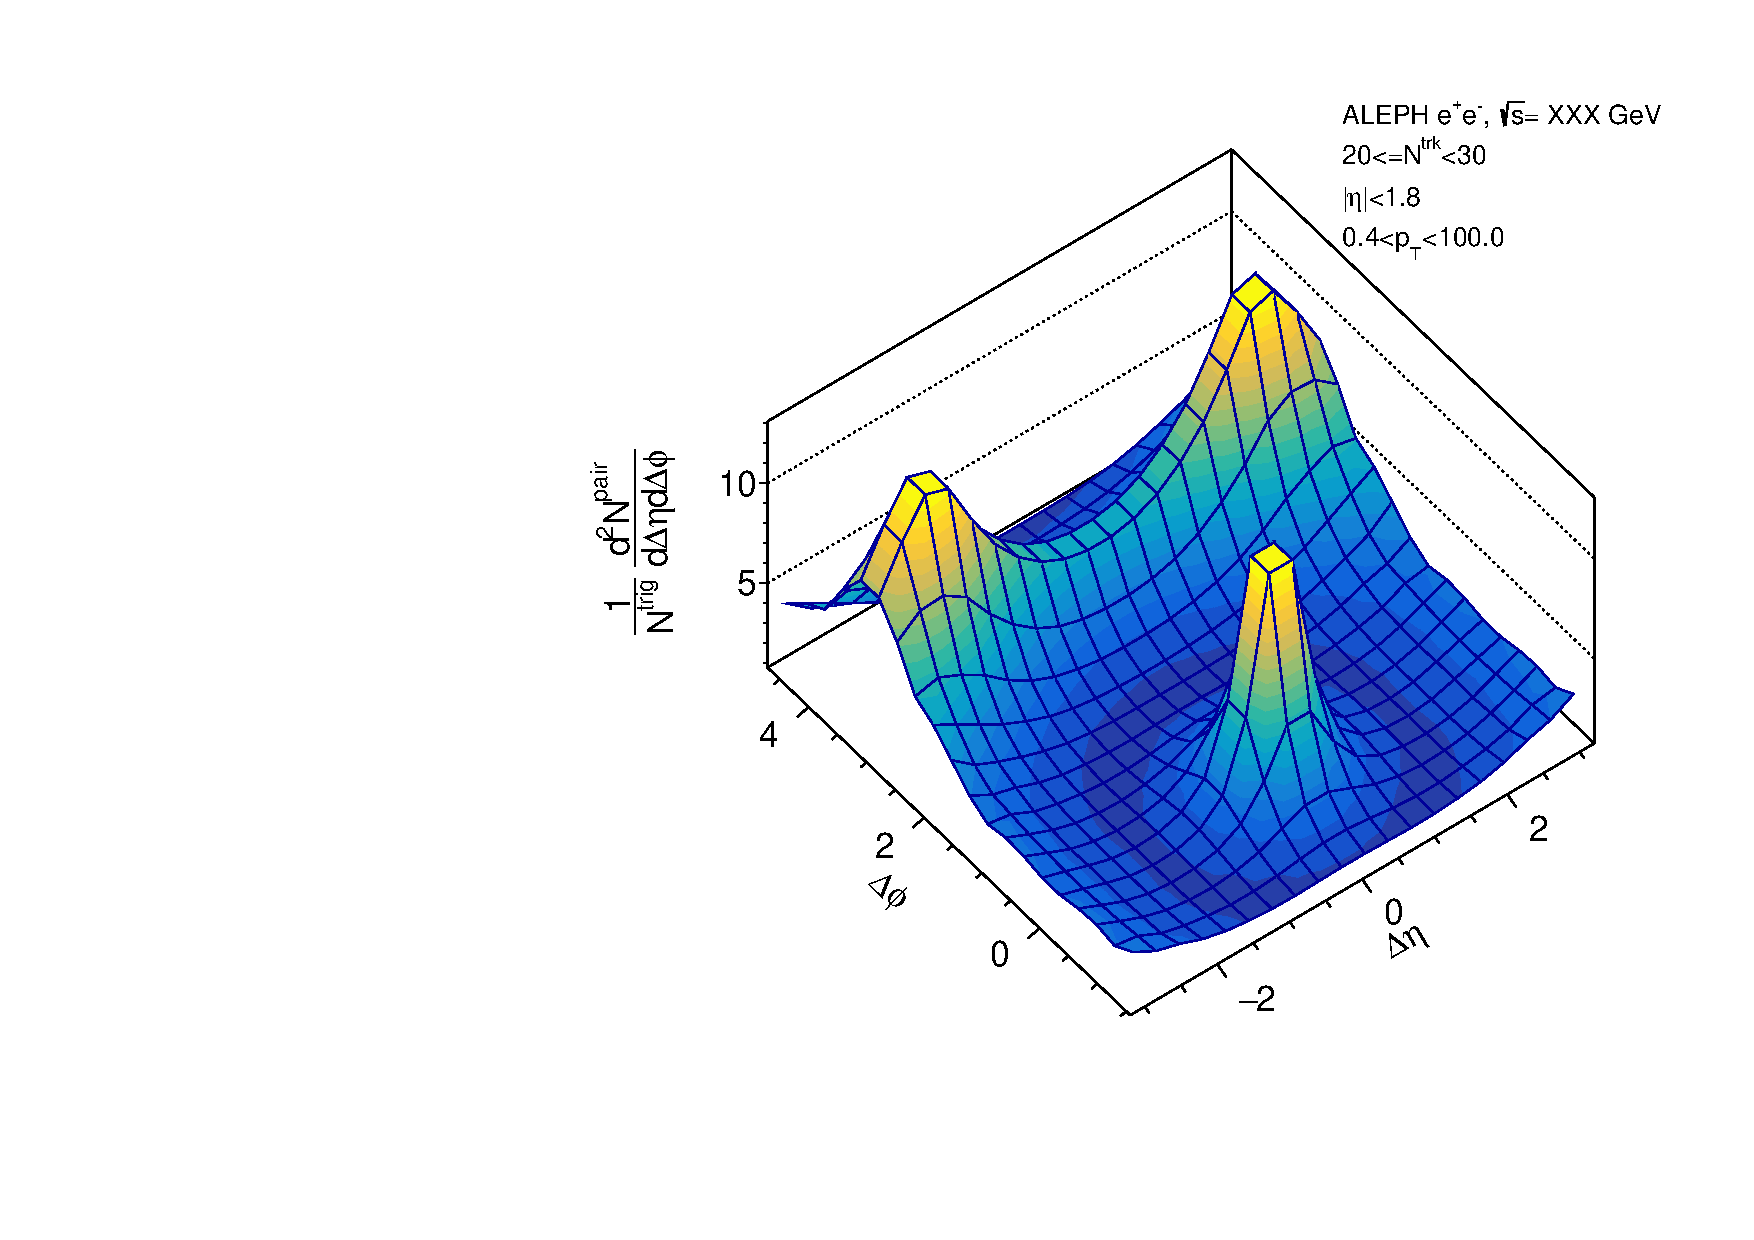
\includegraphics[width=.32\textwidth]{images/TwoParticleCorrelation/CrossCheck/20180126/LEP2_BEAM/LEP2_BEAM_ratio1_20_30.pdf}}\hfill
\subfloat{\label{sfig:f}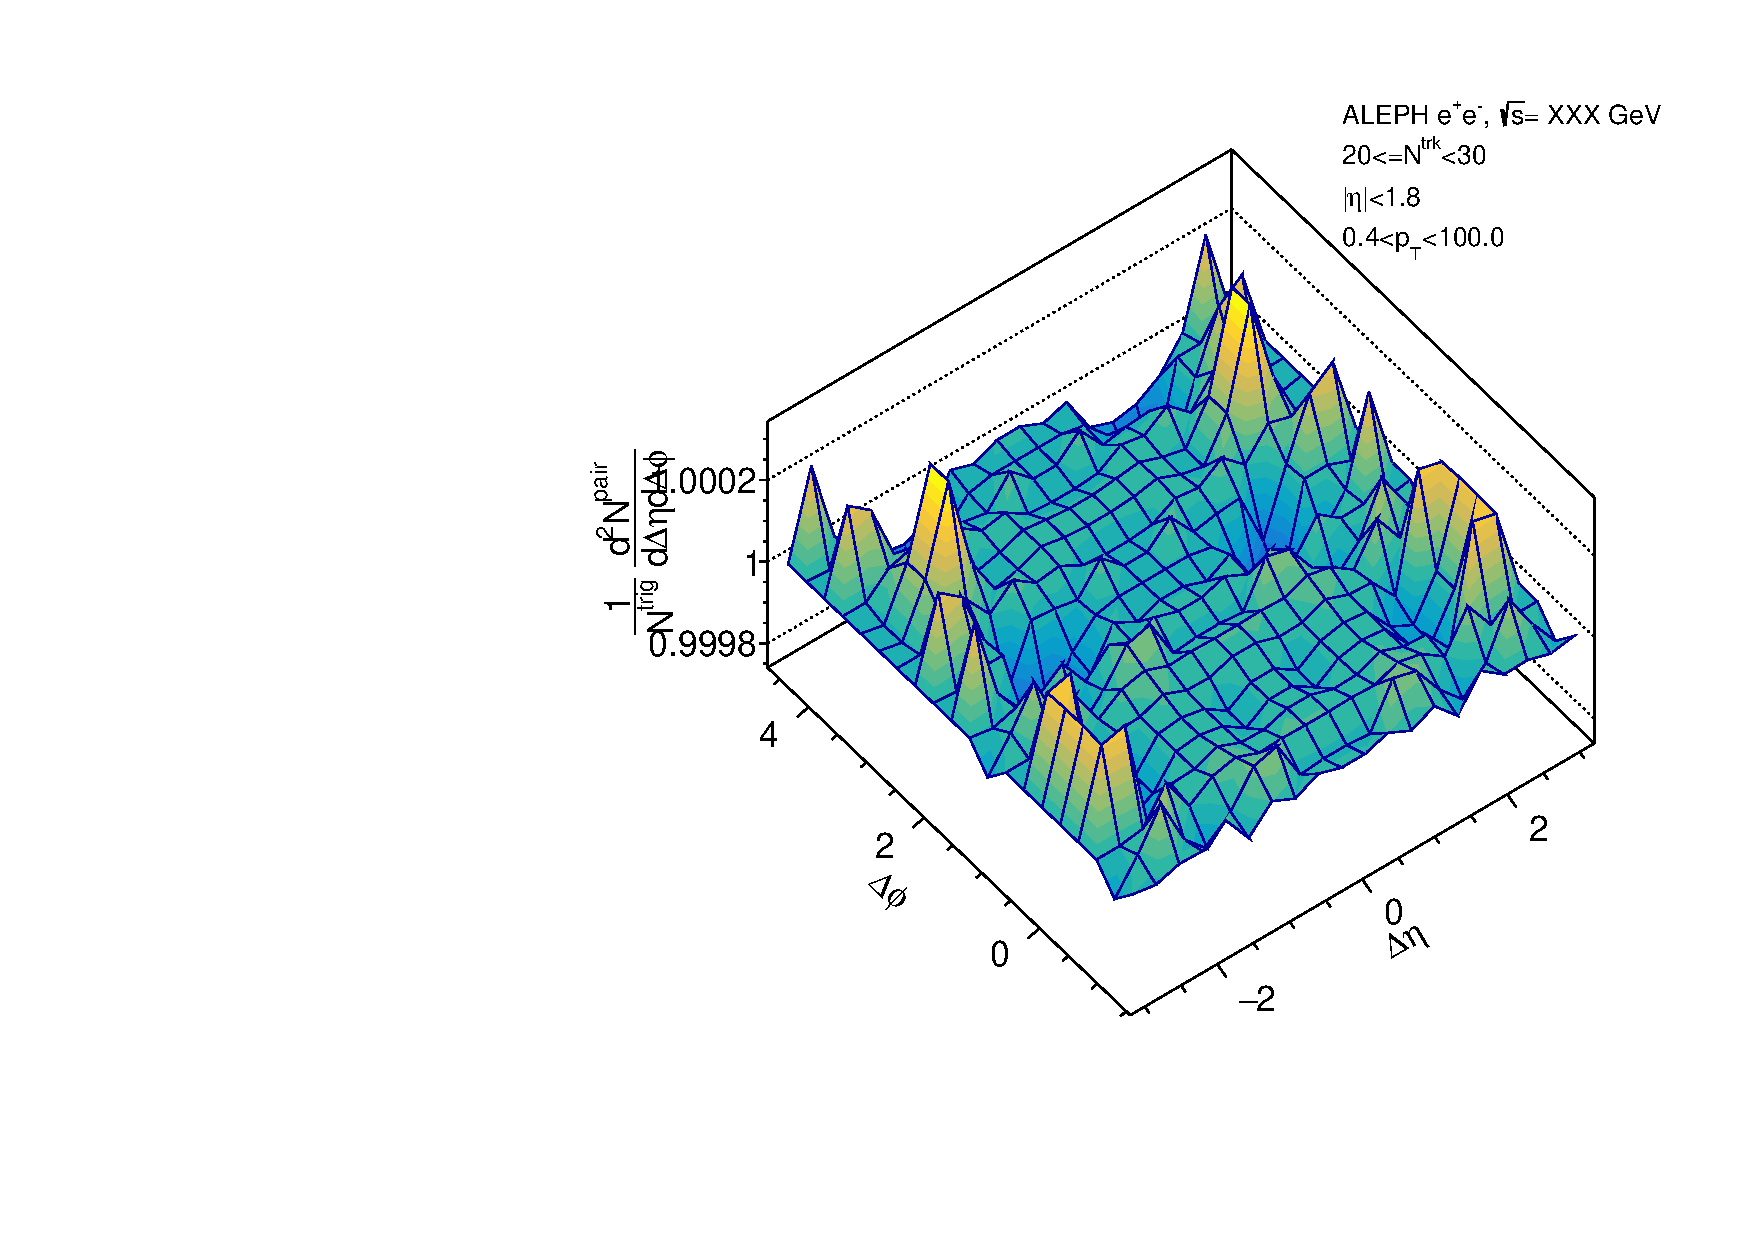
\includegraphics[width=.32\textwidth]{images/TwoParticleCorrelation/CrossCheck/20180126/LEP2_BEAM/LEP2_BEAM_r_ratio_20_30.pdf}}\hfill
\subfloat{\label{sfig:g}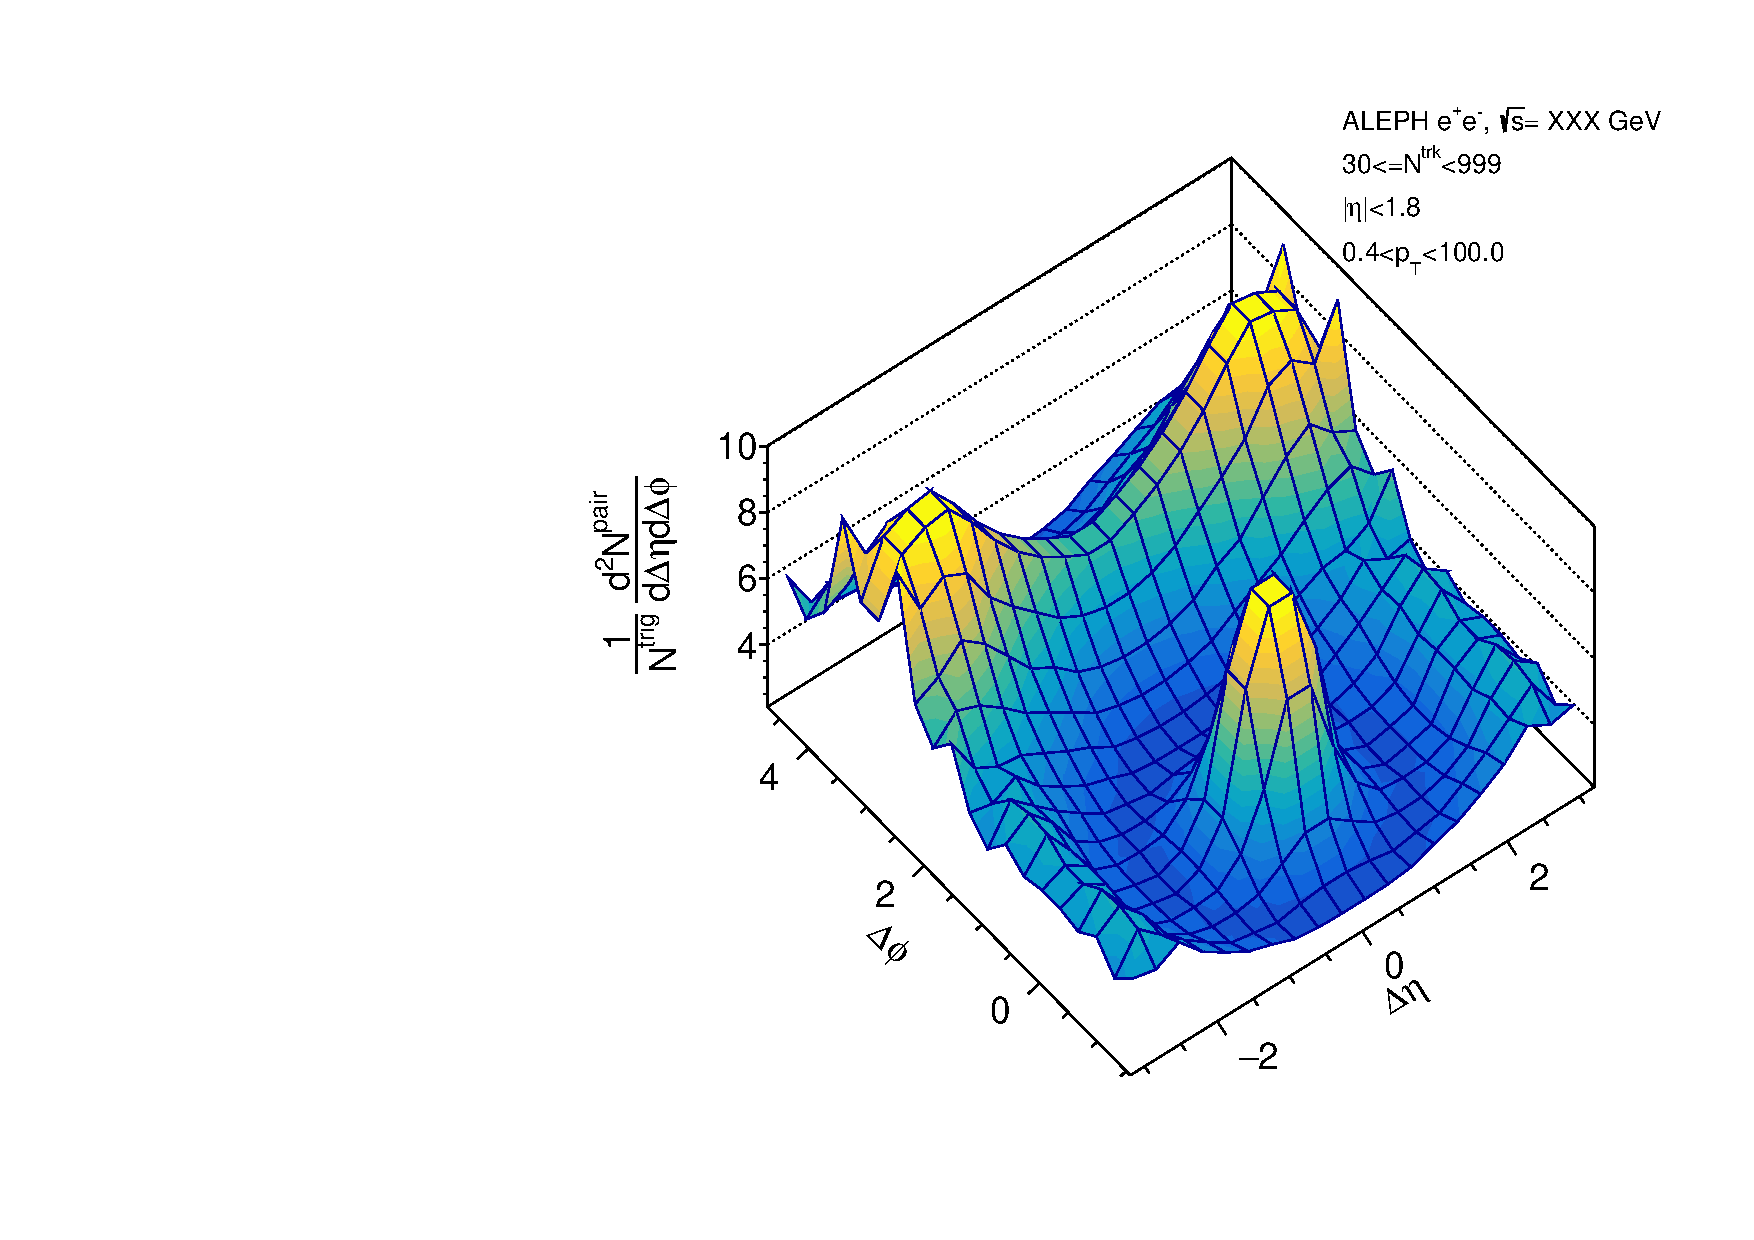
\includegraphics[width=.32\textwidth]{images/TwoParticleCorrelation/CrossCheck/20180126/LEP2_BEAM/LEP2_BEAM_ratio2_30_999.pdf}}\hfill
\subfloat{\label{sfig:h}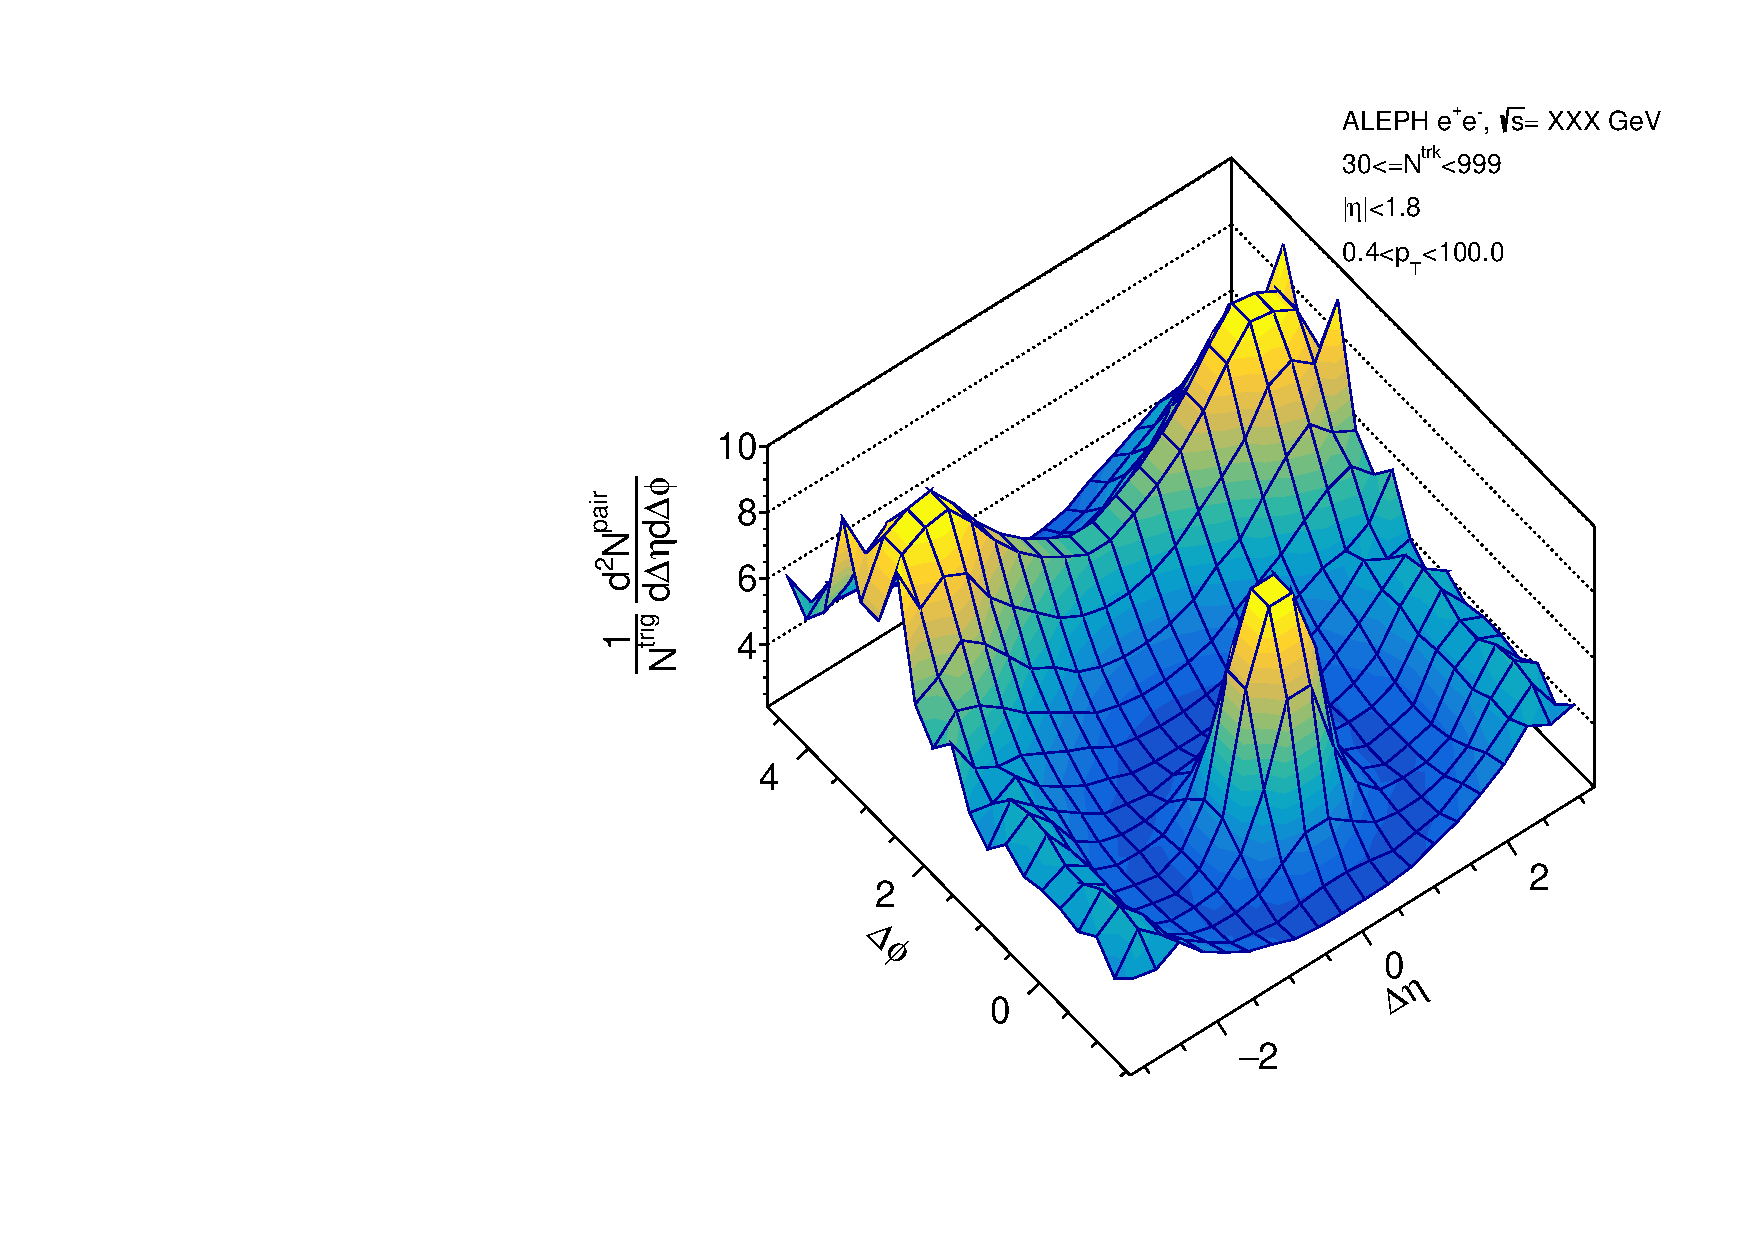
\includegraphics[width=.32\textwidth]{images/TwoParticleCorrelation/CrossCheck/20180126/LEP2_BEAM/LEP2_BEAM_ratio1_30_999.pdf}}\hfill
\subfloat{\label{sfig:i}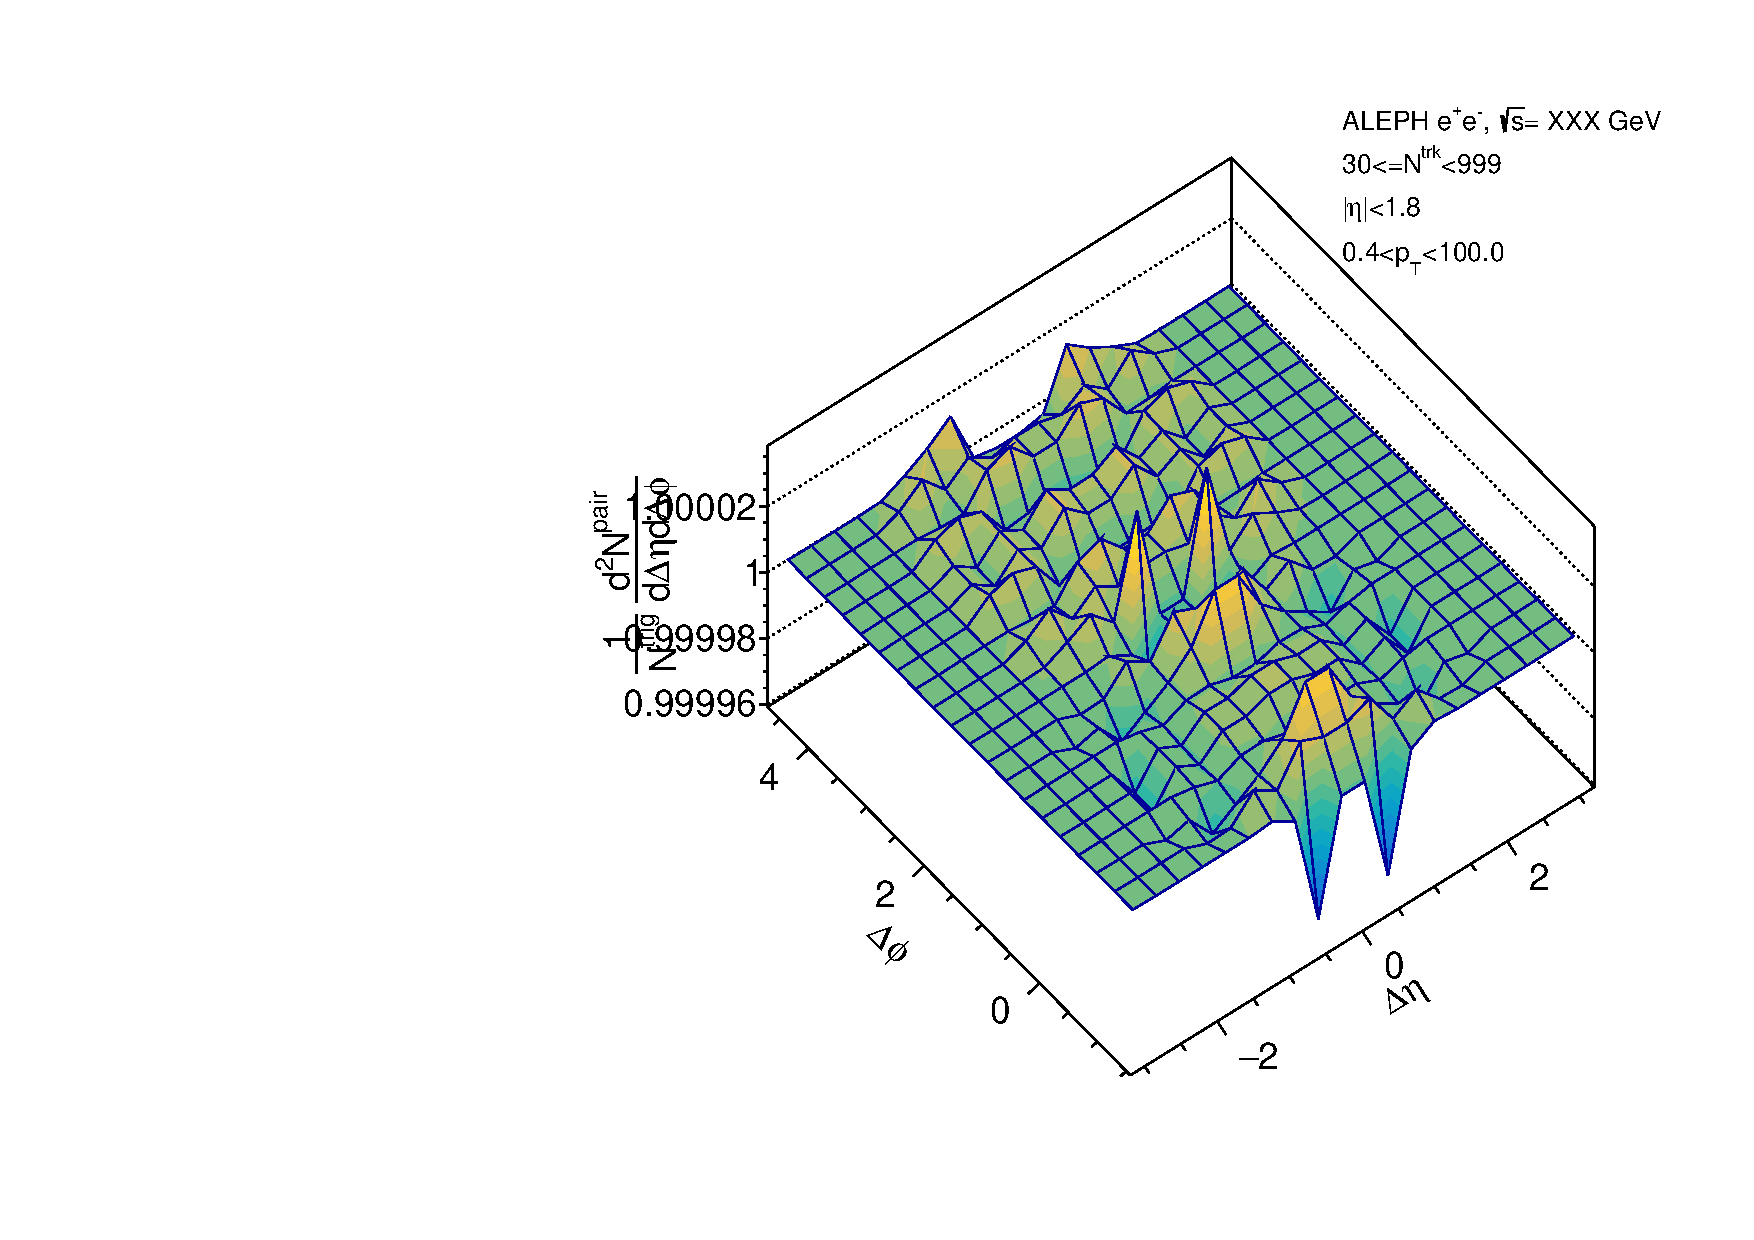
\includegraphics[width=.32\textwidth]{images/TwoParticleCorrelation/CrossCheck/20180126/LEP2_BEAM/LEP2_BEAM_r_ratio_30_999.pdf}} \\
\caption{Two particle correlation fuctions for the LEP2 data set analyzed in the beam axis.}
\label{fig:test}
\end{figure}

\begin{figure}[H]
\centering
\subfloat{\label{sfig:a}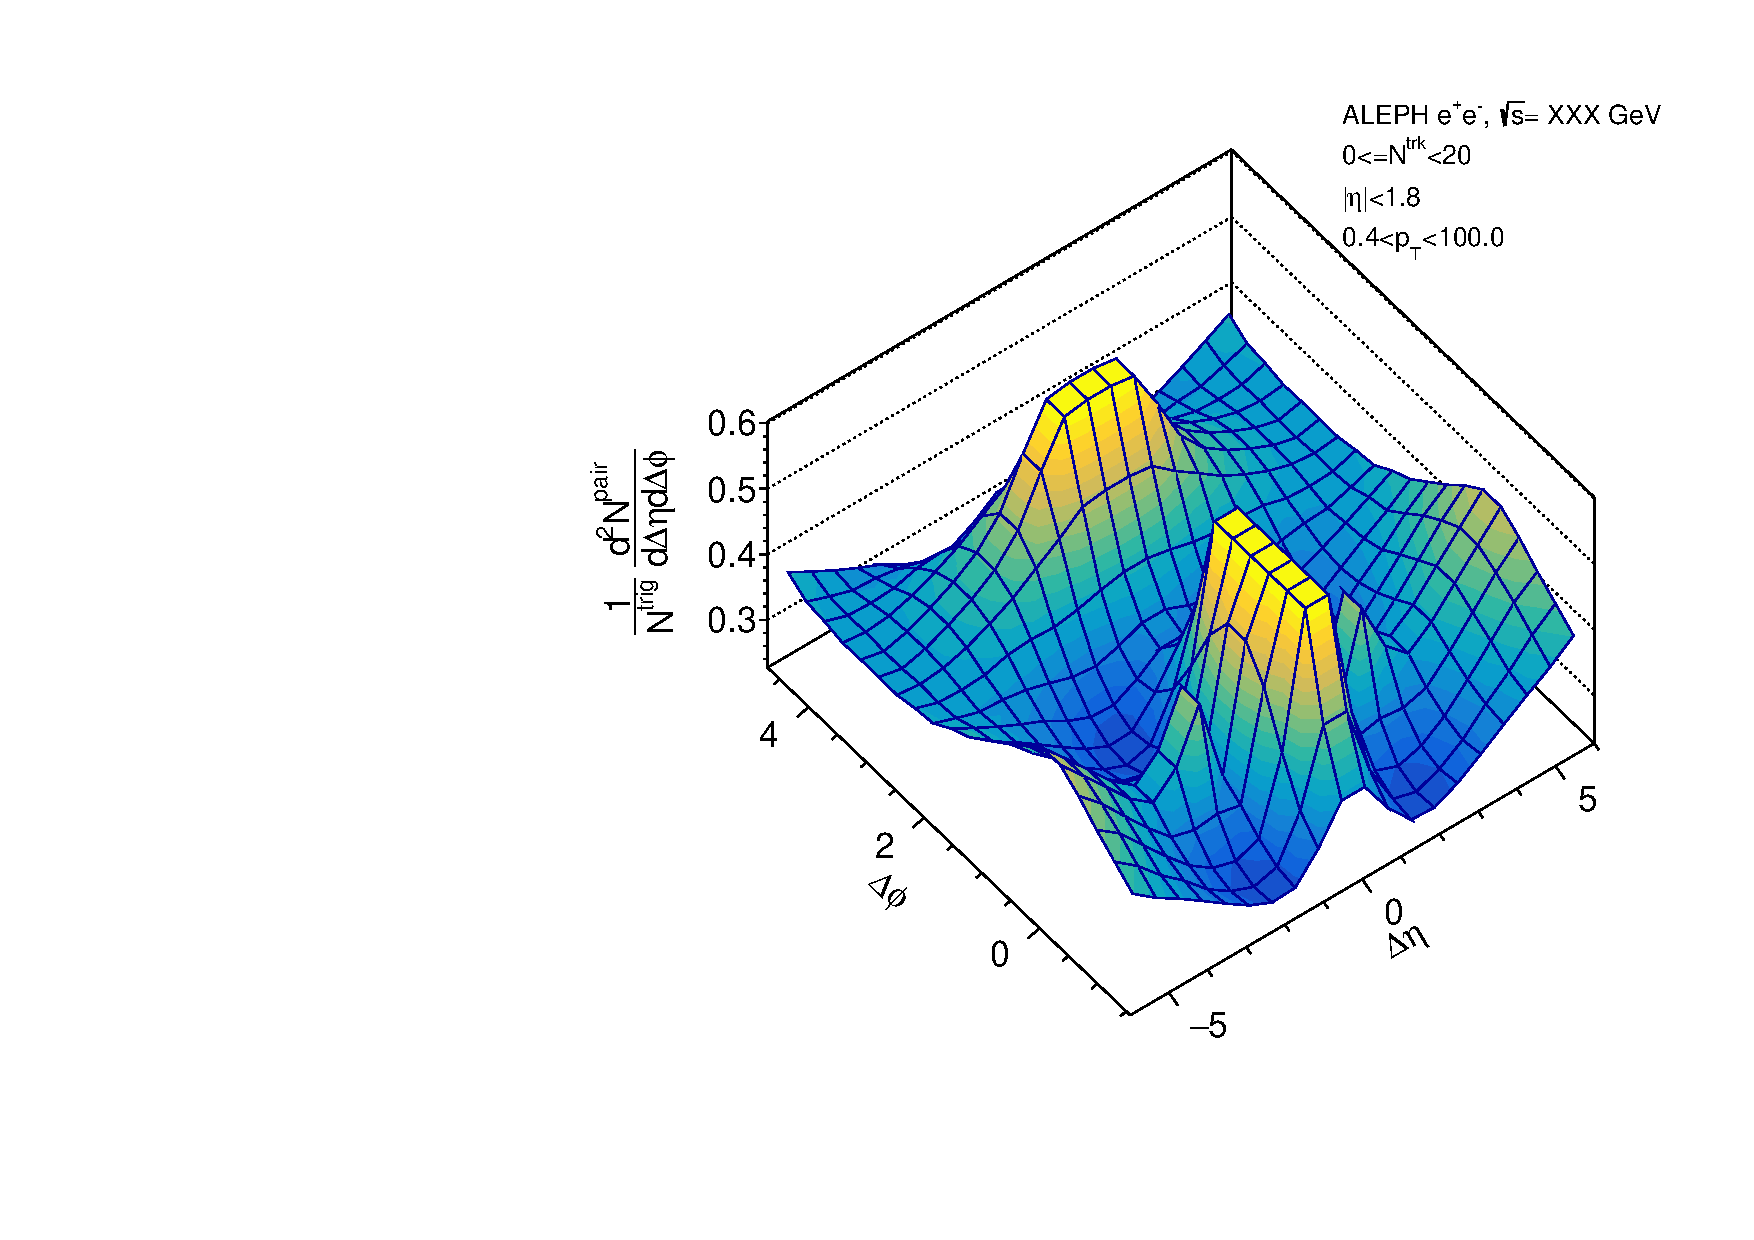
\includegraphics[width=.32\textwidth]{images/TwoParticleCorrelation/CrossCheck/20180126/LEP2_THRUST/LEP2_THRUST_ratio2_0_20.pdf}}\hfill
\subfloat{\label{sfig:b}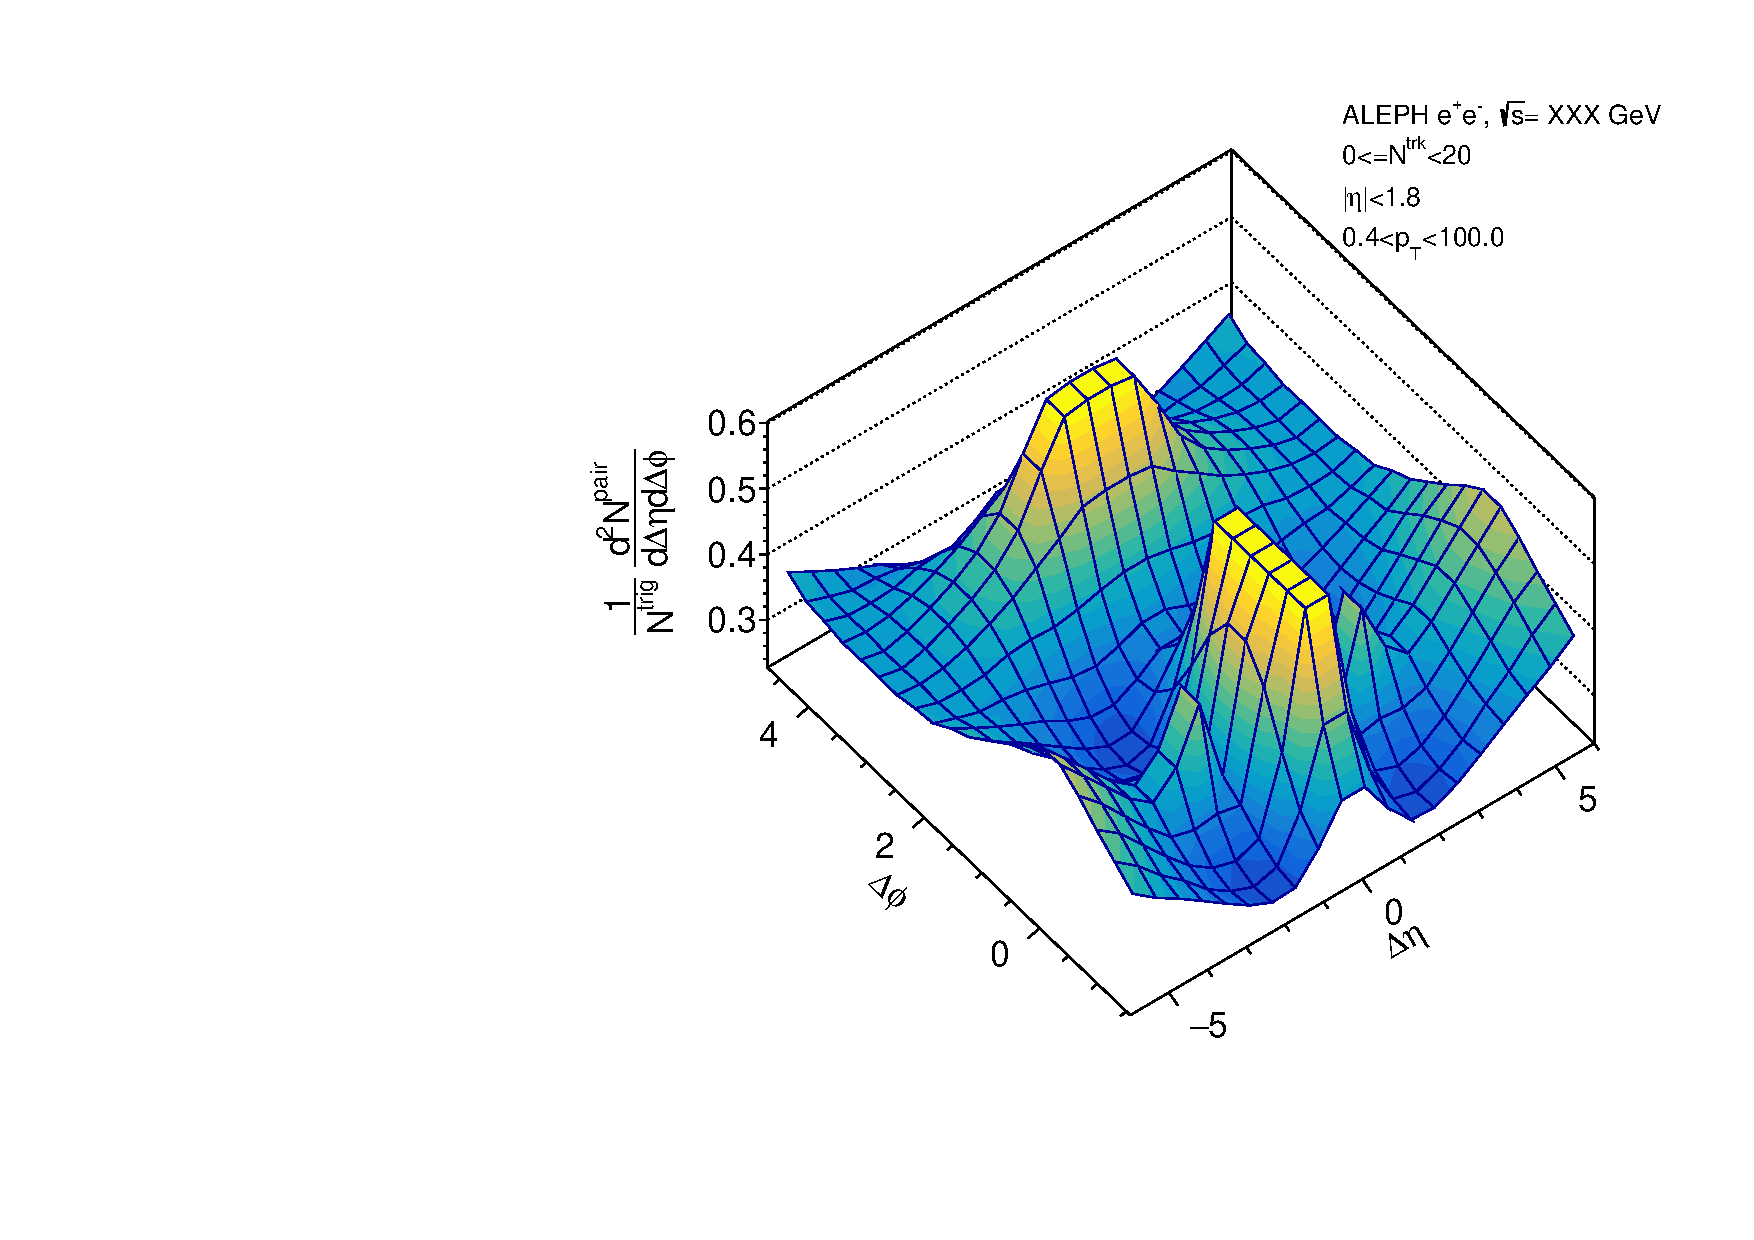
\includegraphics[width=.32\textwidth]{images/TwoParticleCorrelation/CrossCheck/20180126/LEP2_THRUST/LEP2_THRUST_ratio1_0_20.pdf}}\hfill
\subfloat{\label{sfig:c}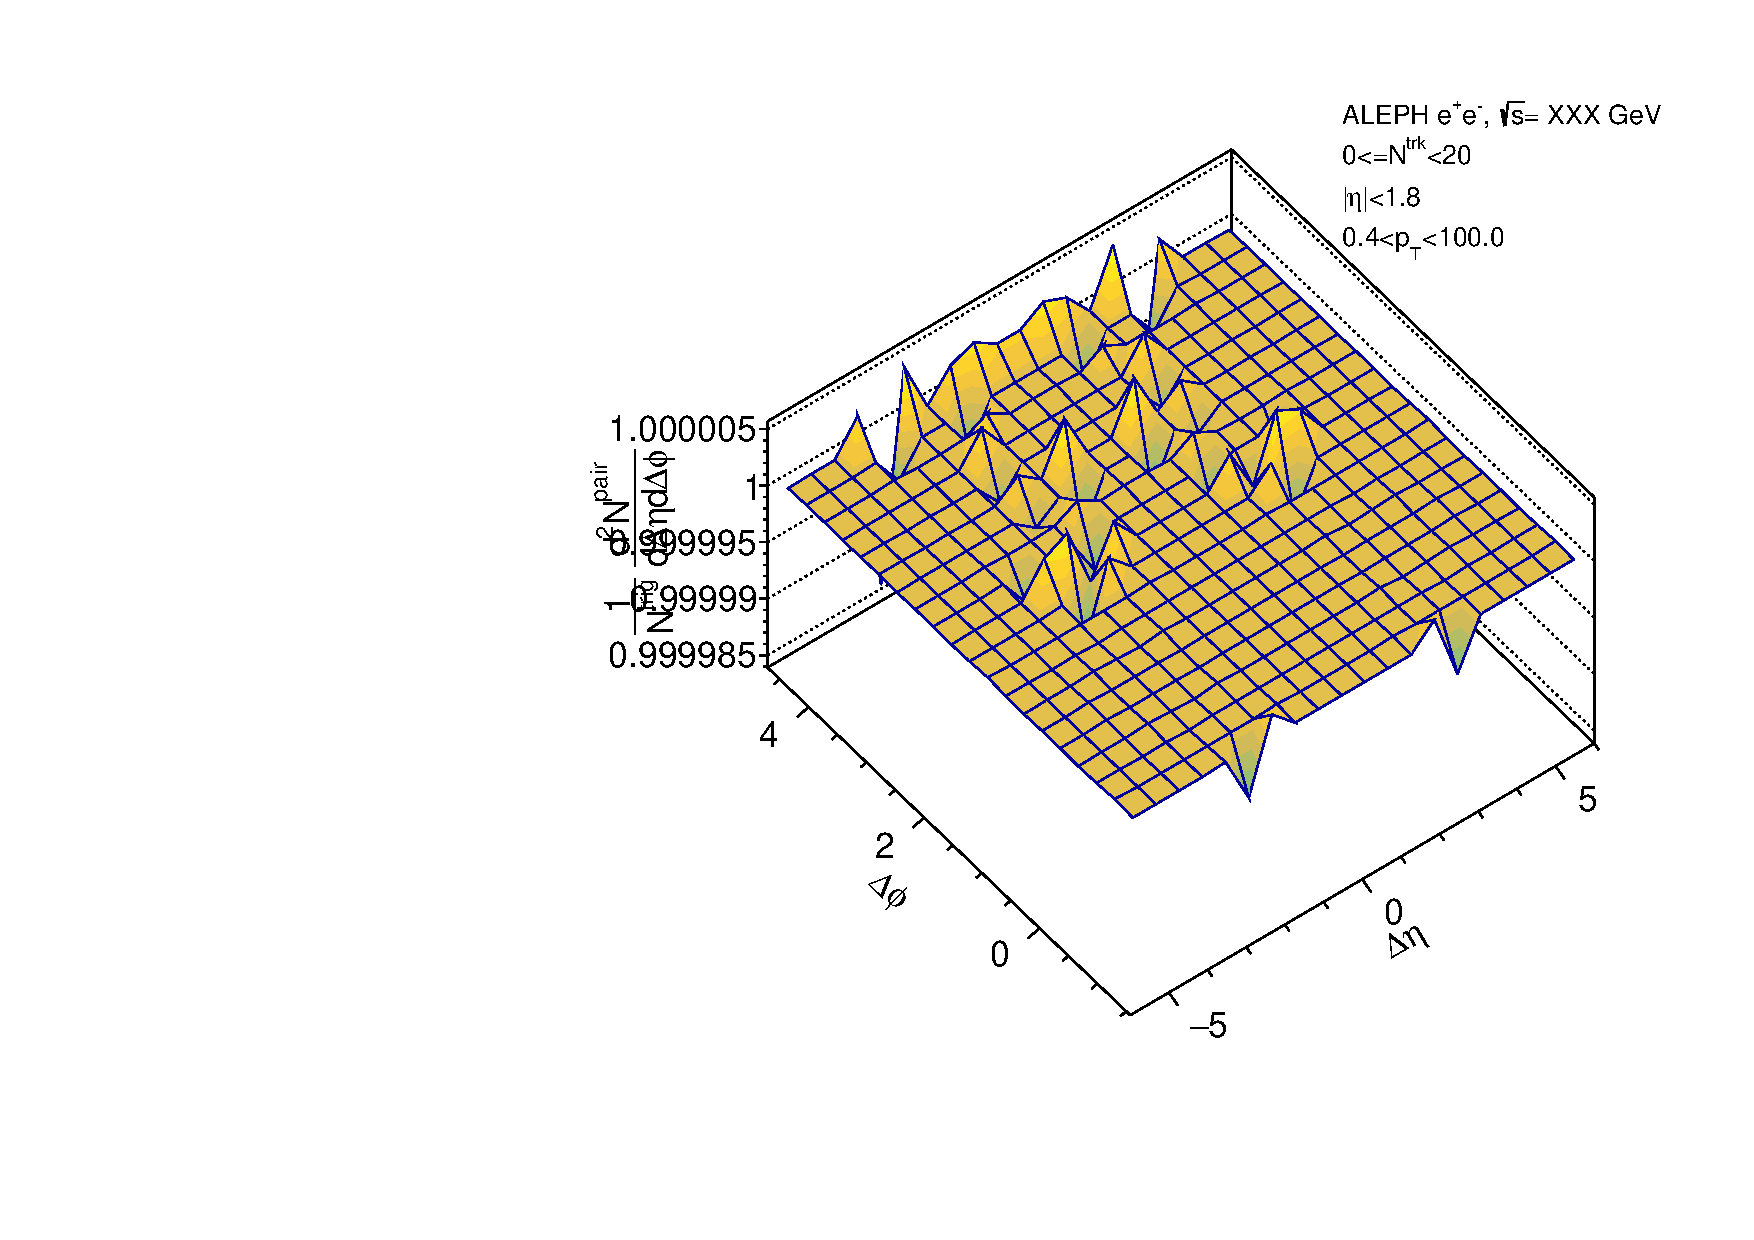
\includegraphics[width=.32\textwidth]{images/TwoParticleCorrelation/CrossCheck/20180126/LEP2_THRUST/LEP2_THRUST_r_ratio_0_20.pdf}}\hfill
\subfloat{\label{sfig:d}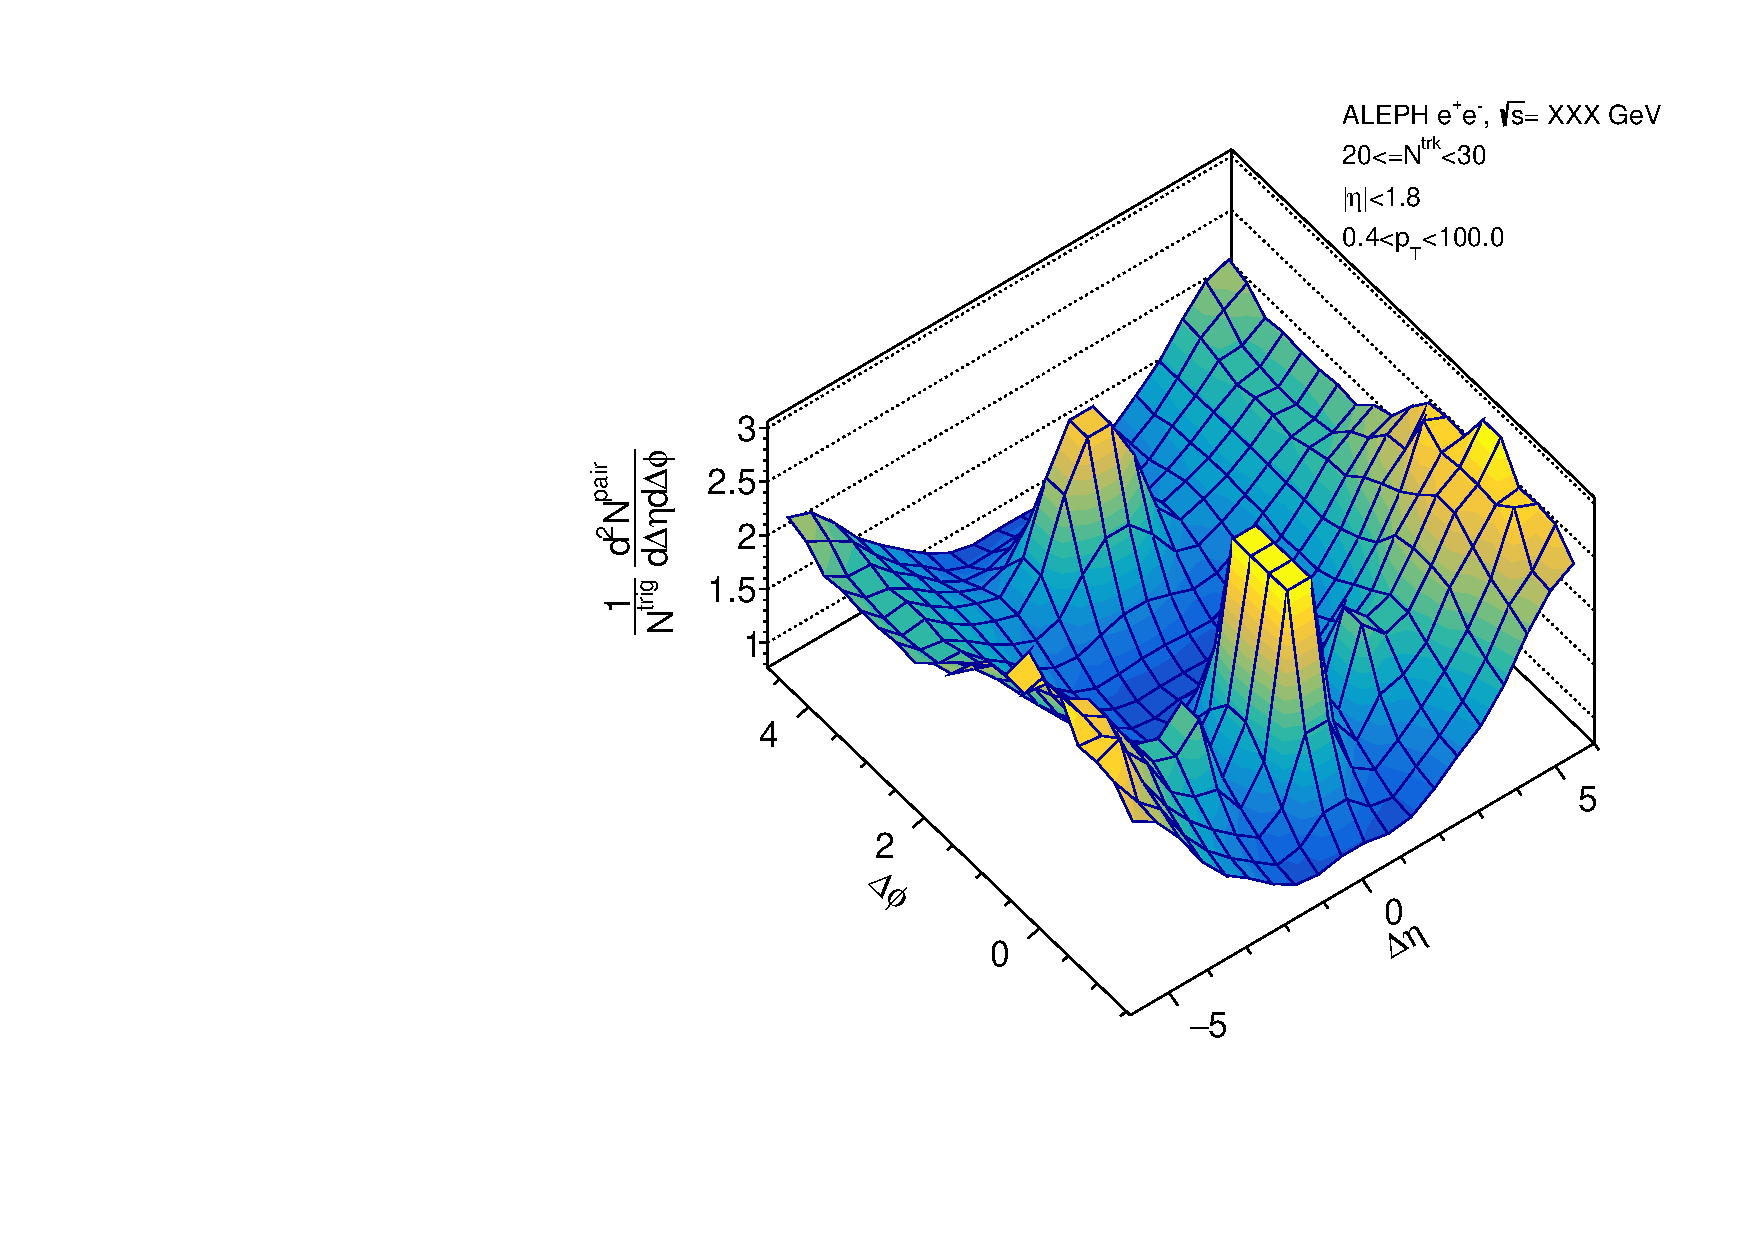
\includegraphics[width=.32\textwidth]{images/TwoParticleCorrelation/CrossCheck/20180126/LEP2_THRUST/LEP2_THRUST_ratio2_20_30.pdf}}\hfill
\subfloat{\label{sfig:e}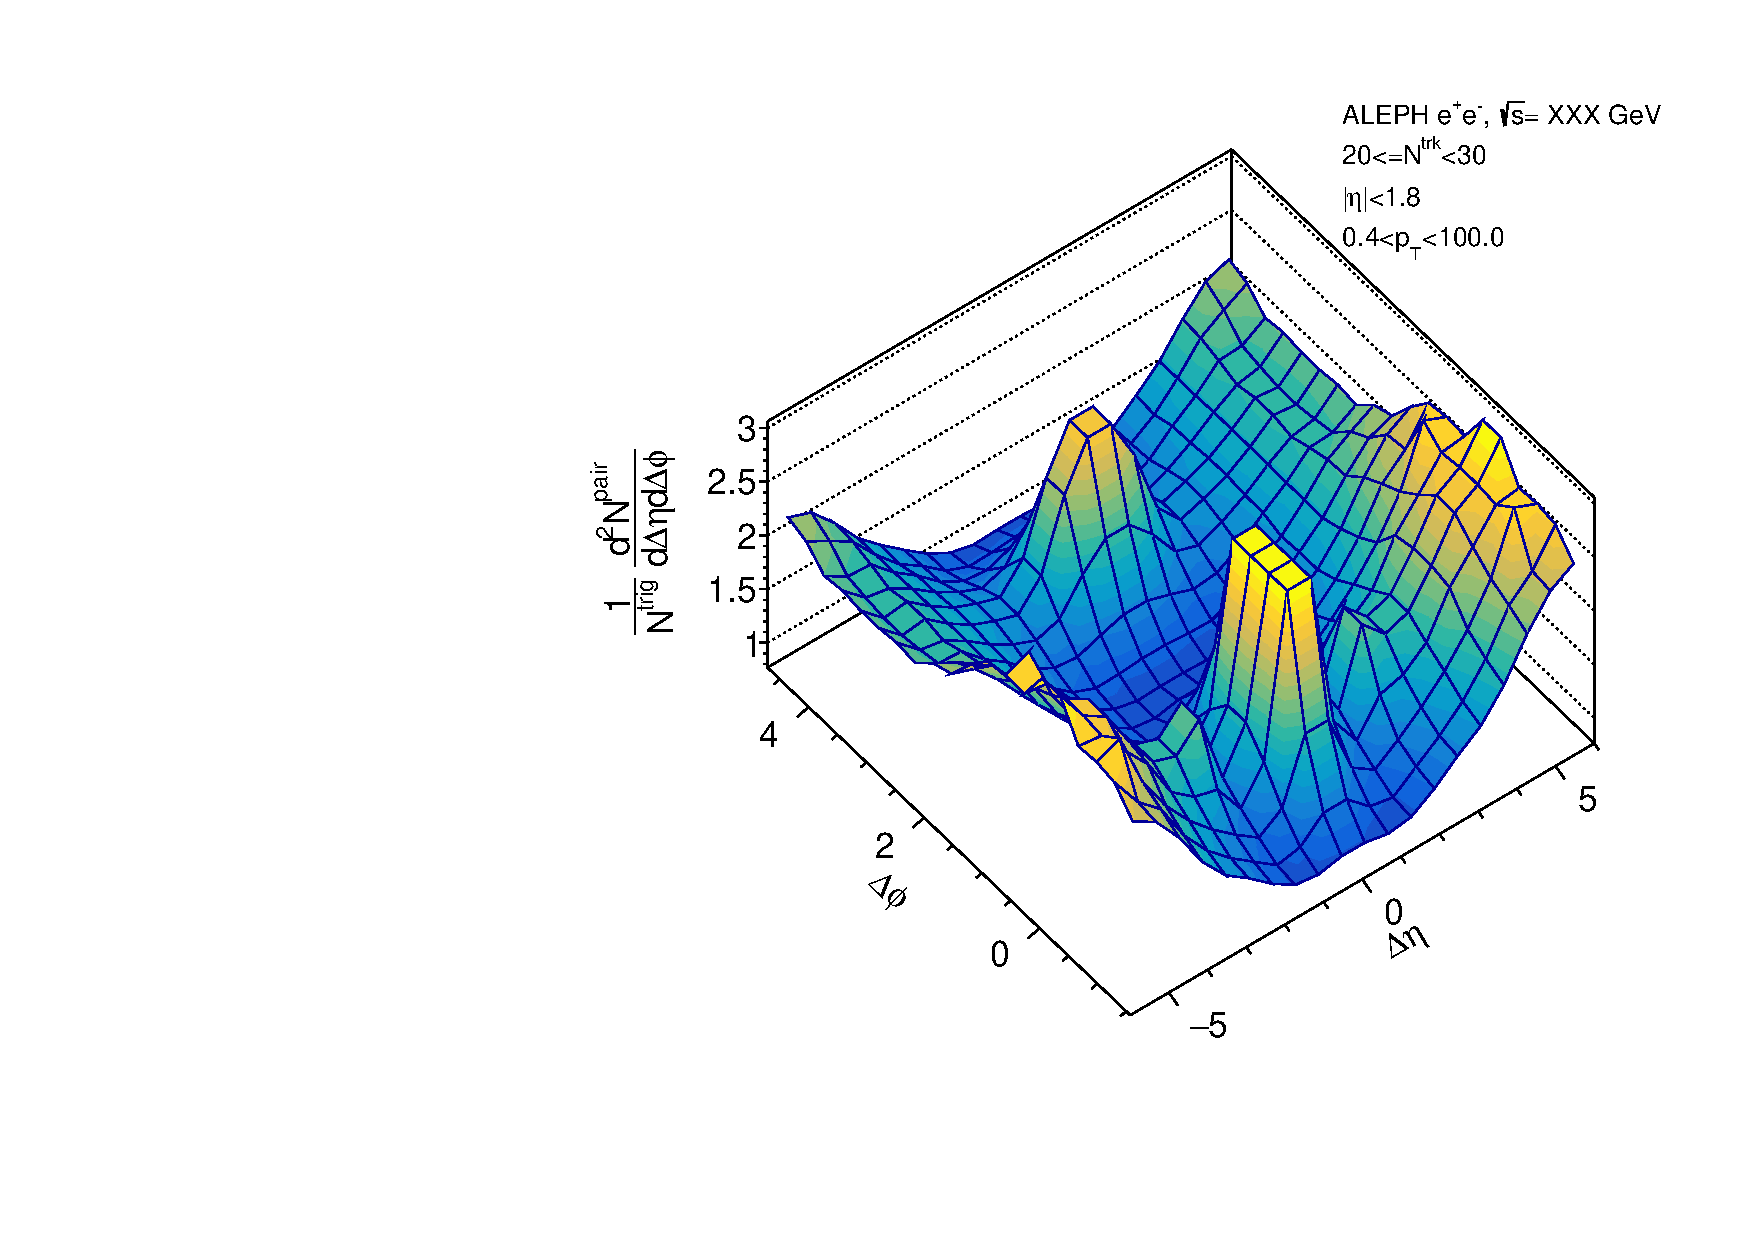
\includegraphics[width=.32\textwidth]{images/TwoParticleCorrelation/CrossCheck/20180126/LEP2_THRUST/LEP2_THRUST_ratio1_20_30.pdf}}\hfill
\subfloat{\label{sfig:f}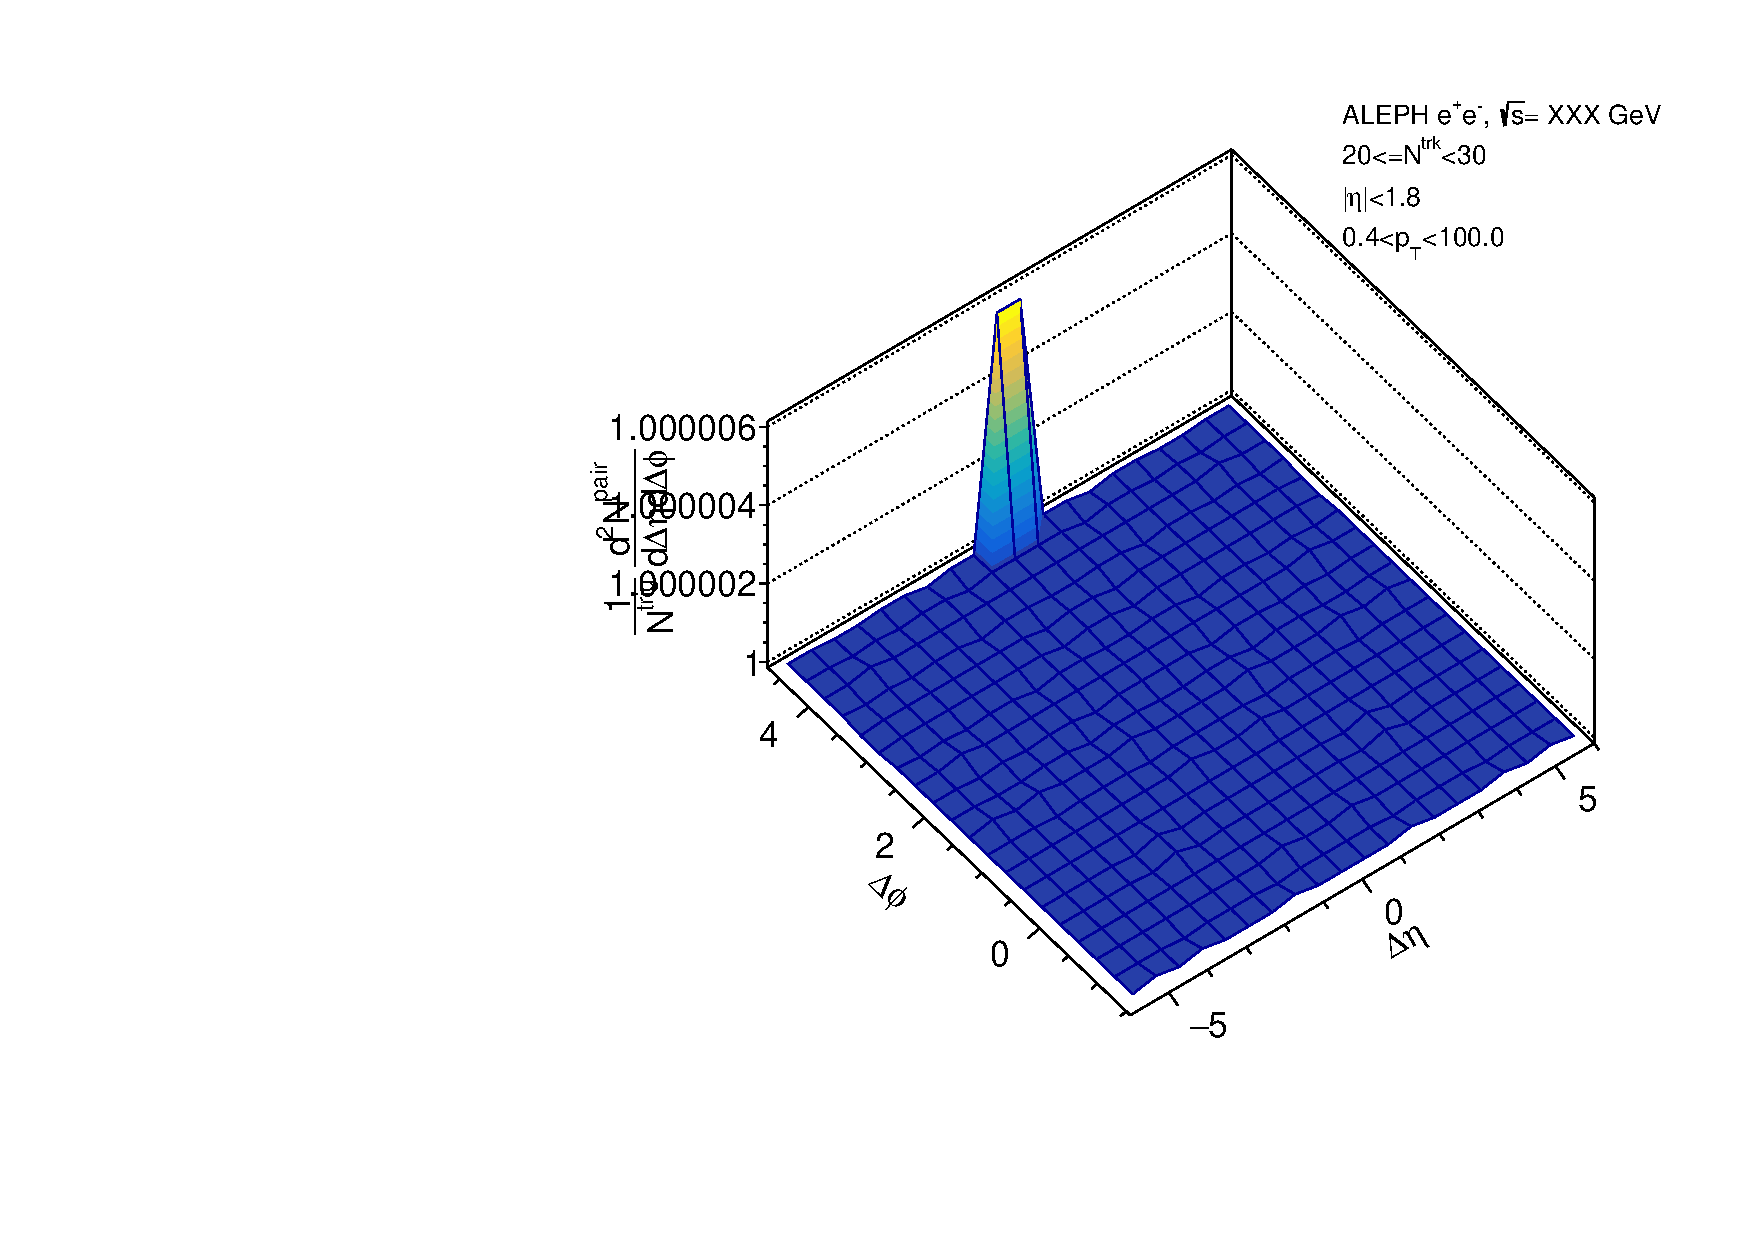
\includegraphics[width=.32\textwidth]{images/TwoParticleCorrelation/CrossCheck/20180126/LEP2_THRUST/LEP2_THRUST_r_ratio_20_30.pdf}}\hfill
\subfloat{\label{sfig:g}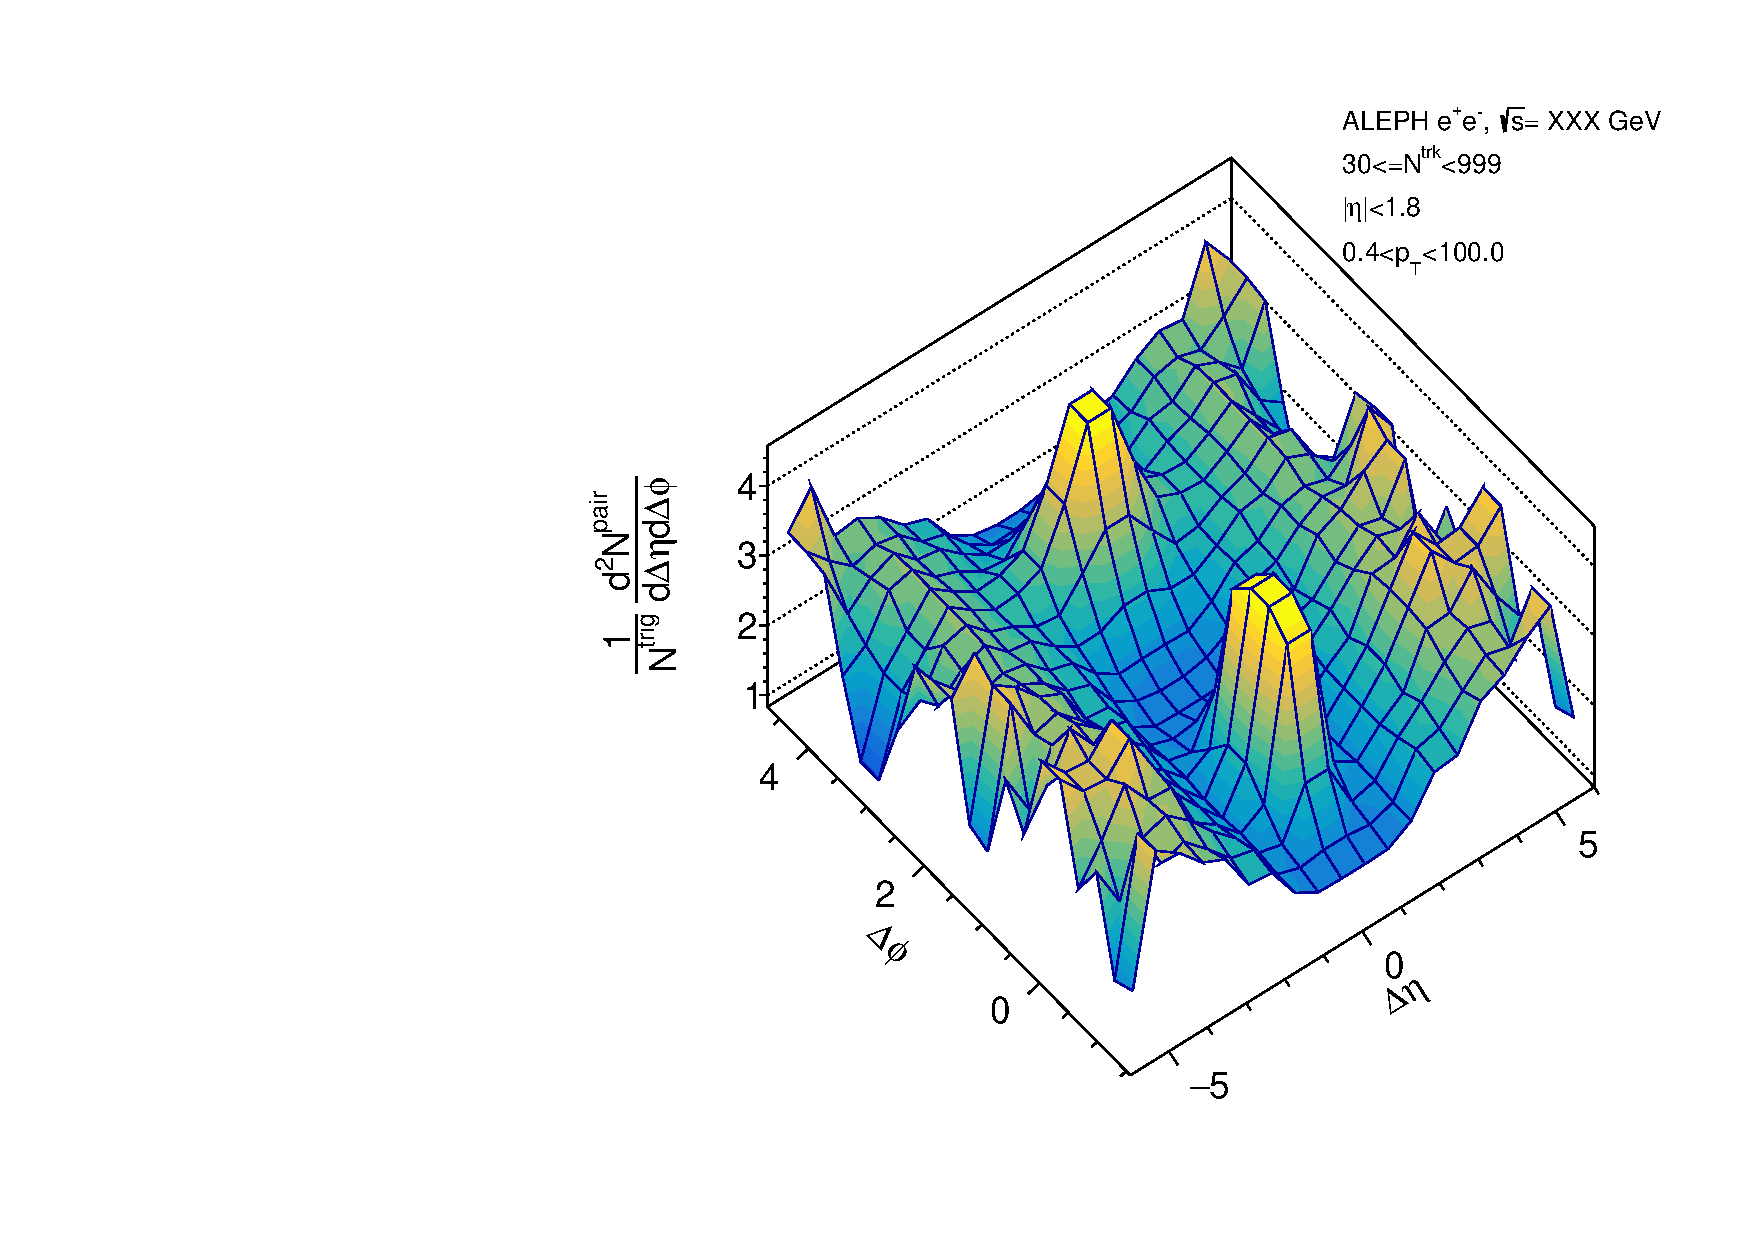
\includegraphics[width=.32\textwidth]{images/TwoParticleCorrelation/CrossCheck/20180126/LEP2_THRUST/LEP2_THRUST_ratio2_30_999.pdf}}\hfill
\subfloat{\label{sfig:h}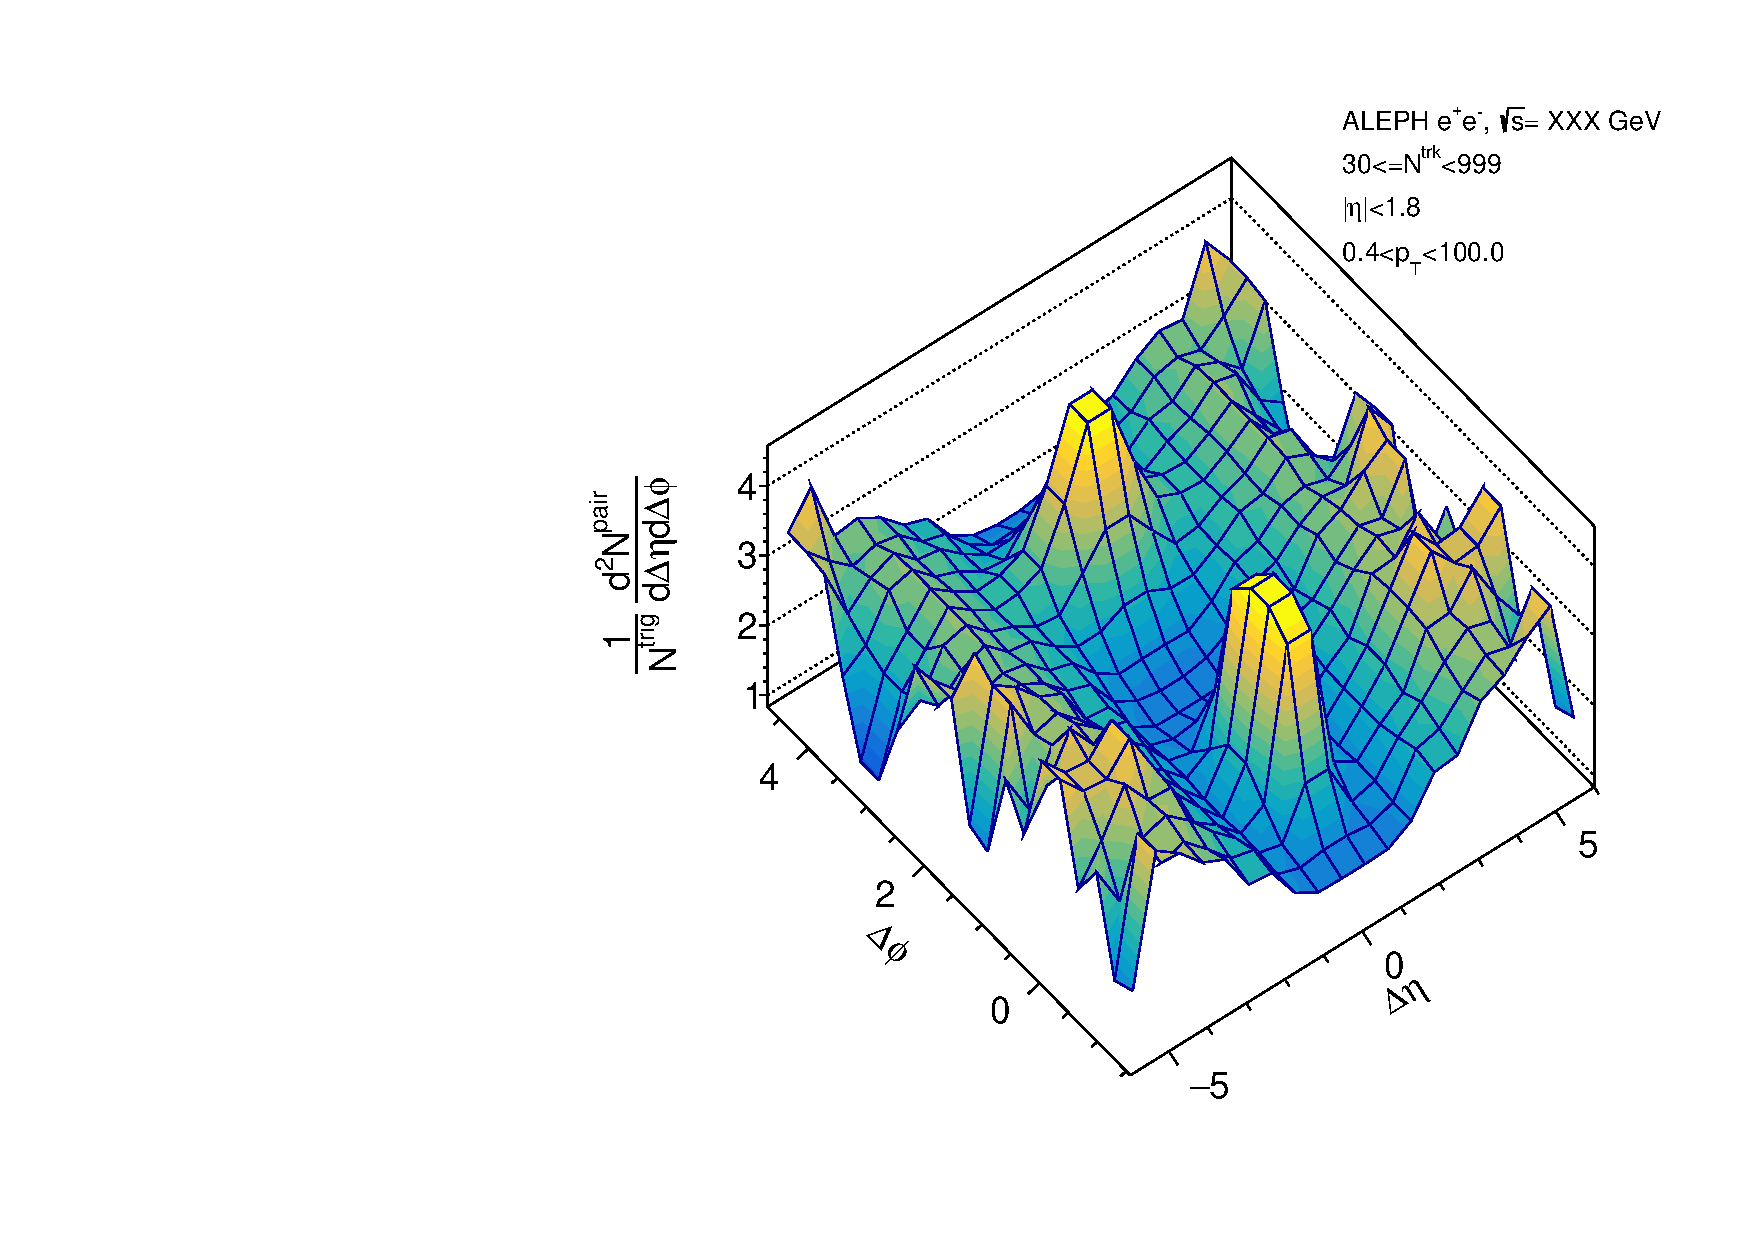
\includegraphics[width=.32\textwidth]{images/TwoParticleCorrelation/CrossCheck/20180126/LEP2_THRUST/LEP2_THRUST_ratio1_30_999.pdf}}\hfill
\subfloat{\label{sfig:i}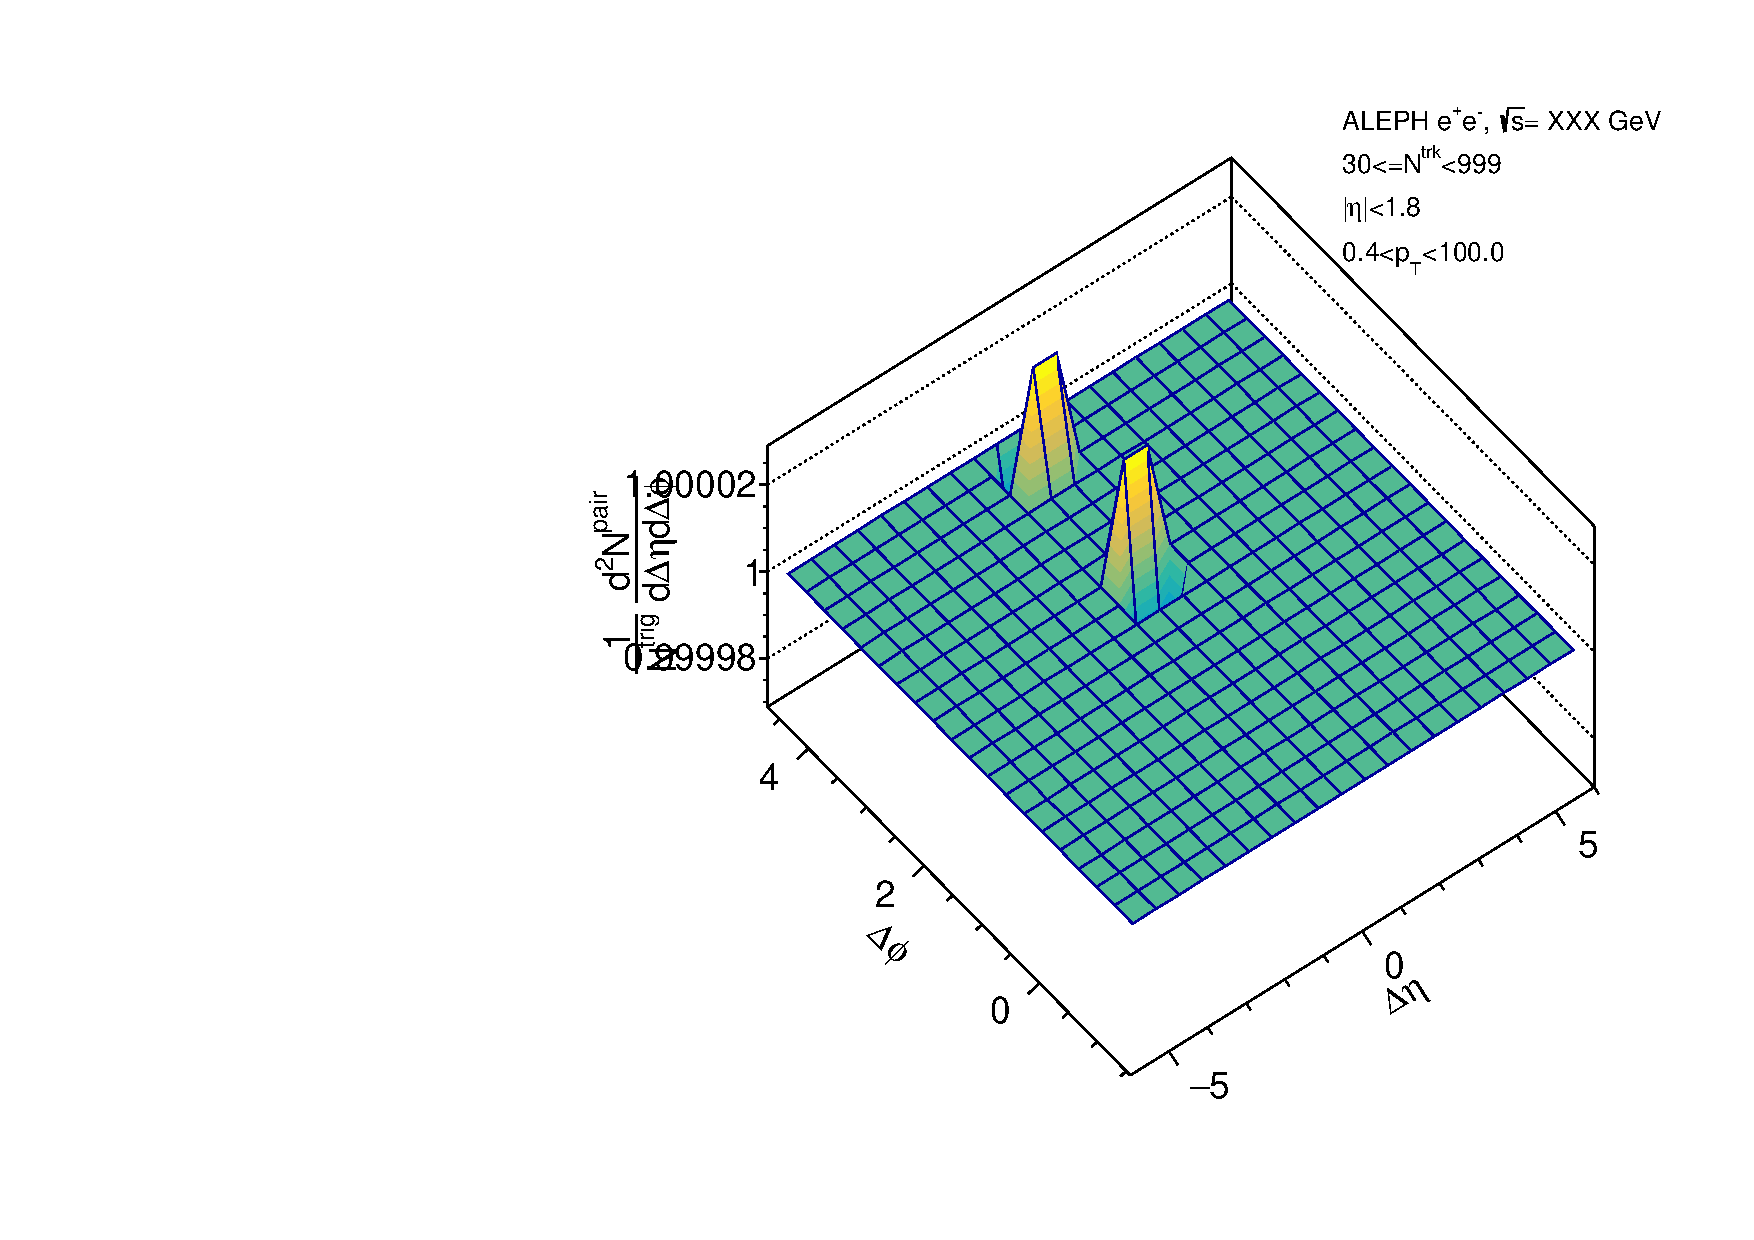
\includegraphics[width=.32\textwidth]{images/TwoParticleCorrelation/CrossCheck/20180126/LEP2_THRUST/LEP2_THRUST_r_ratio_30_999.pdf}} \\
\caption{Two particle correlation fuctions for the LEP2 data set analyzed in the thrust axis.}
\label{fig:test}
\end{figure}

\begin{figure}[H]
\centering
\subfloat{\label{sfig:a}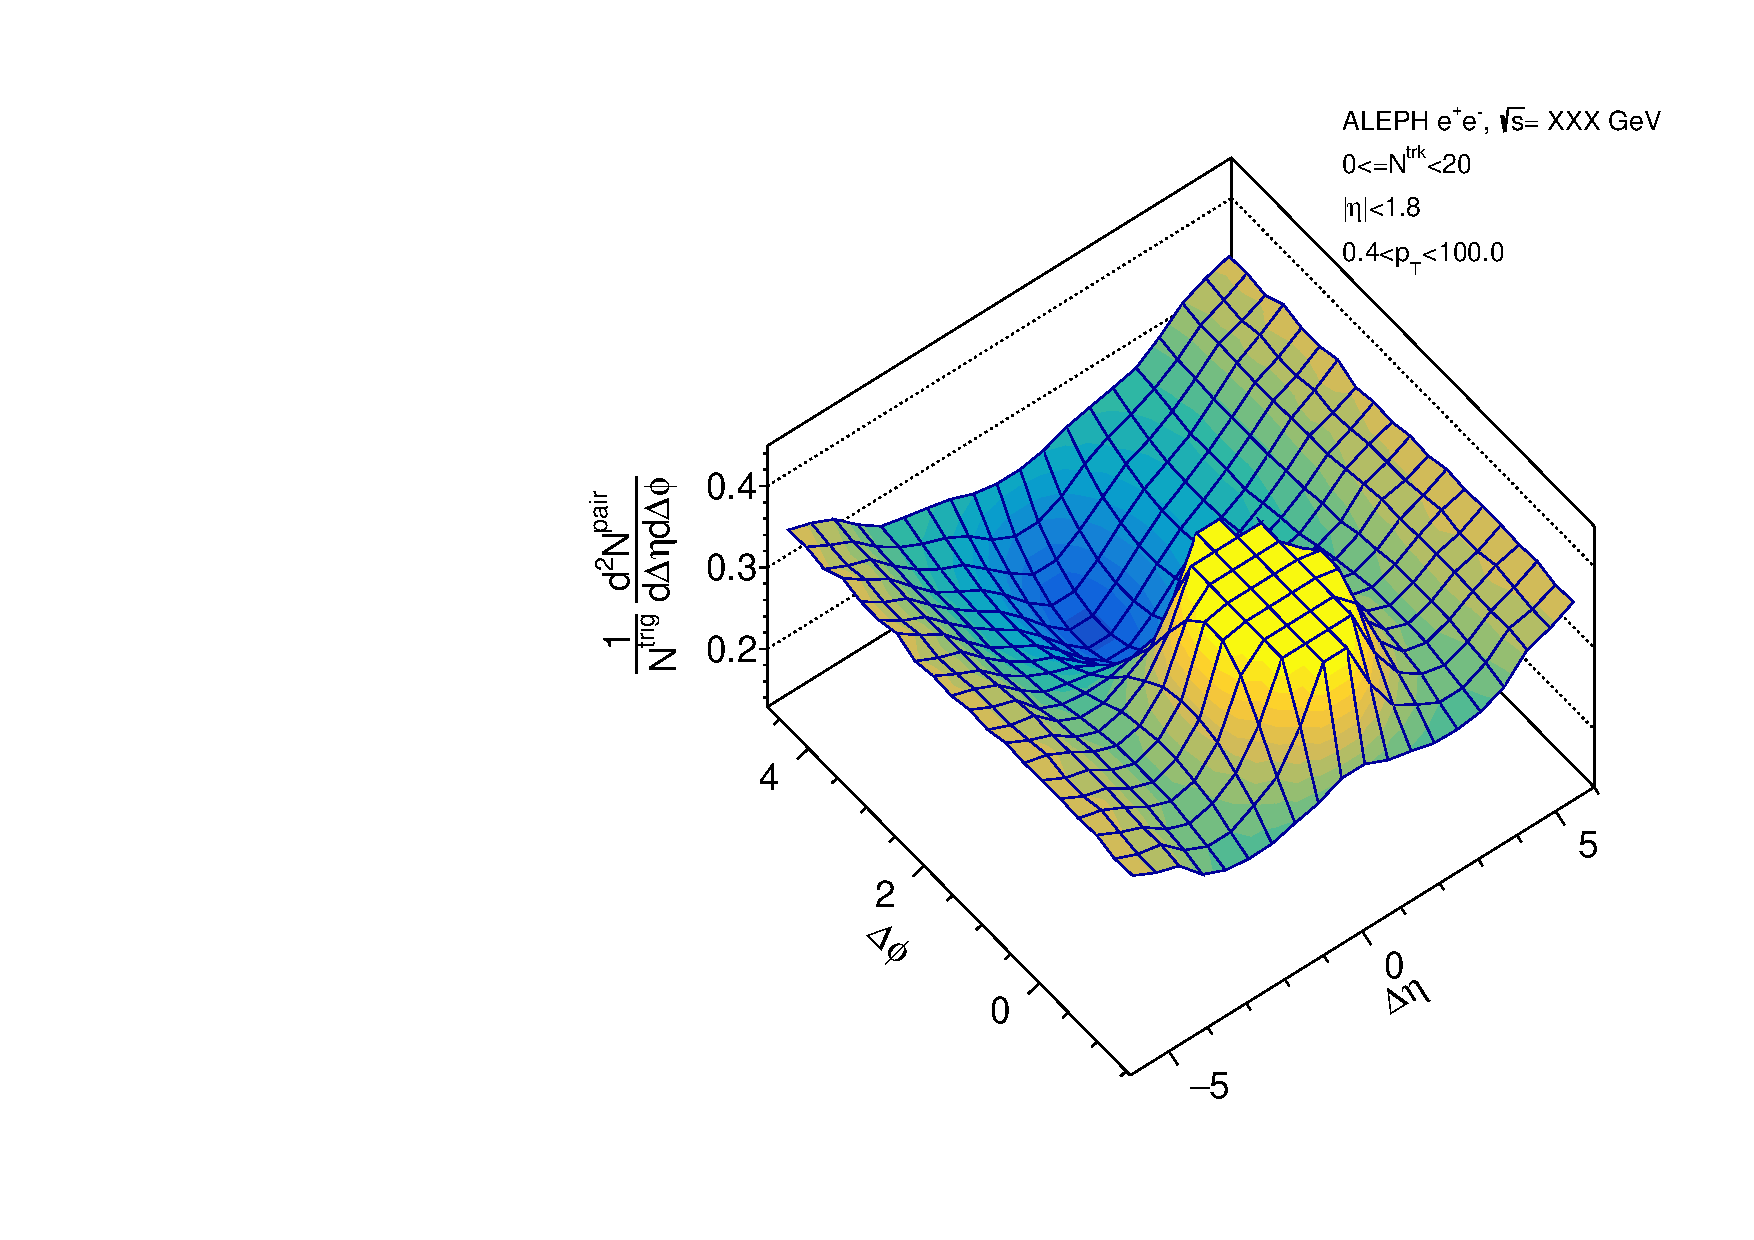
\includegraphics[width=.32\textwidth]{images/TwoParticleCorrelation/CrossCheck/20180126/LEP2_WTA/LEP2_WTA_ratio2_0_20.pdf}}\hfill
\subfloat{\label{sfig:b}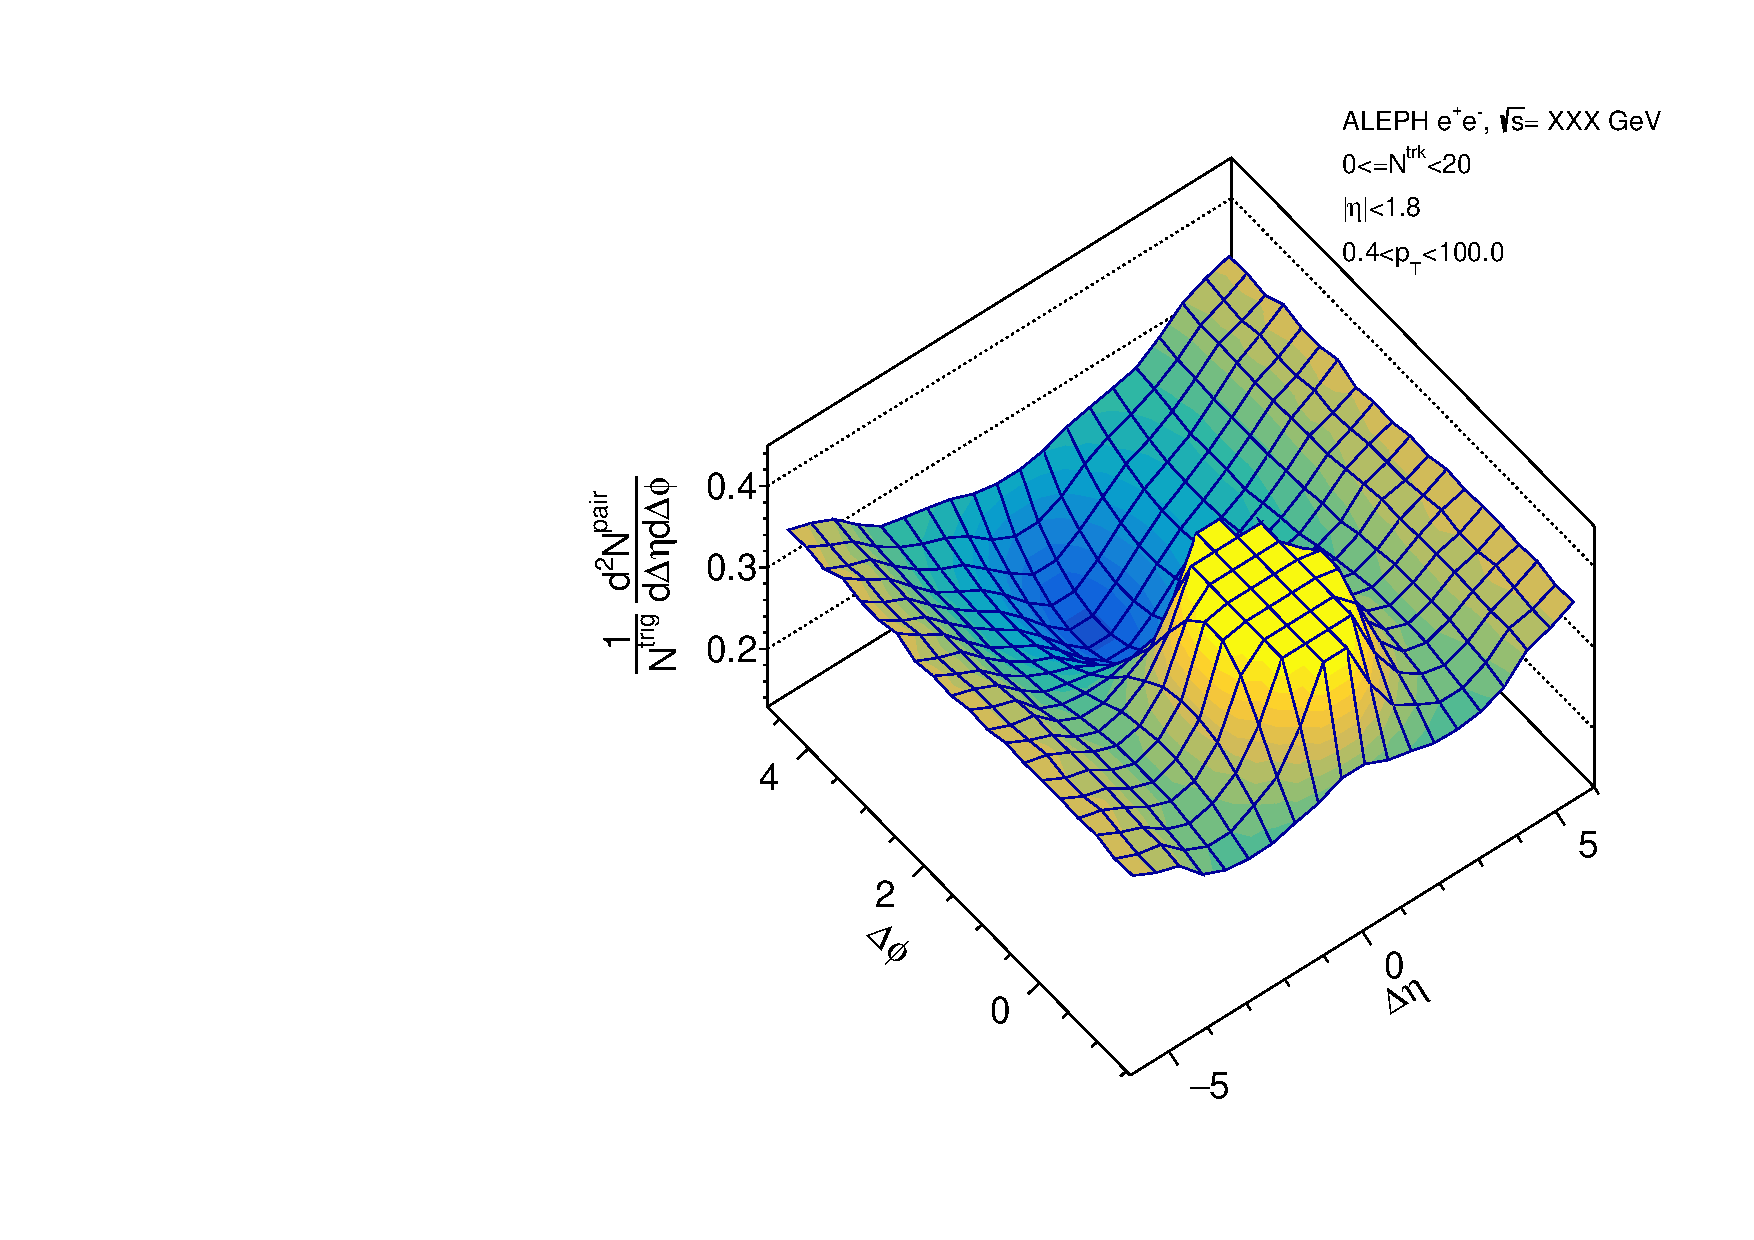
\includegraphics[width=.32\textwidth]{images/TwoParticleCorrelation/CrossCheck/20180126/LEP2_WTA/LEP2_WTA_ratio1_0_20.pdf}}\hfill
\subfloat{\label{sfig:c}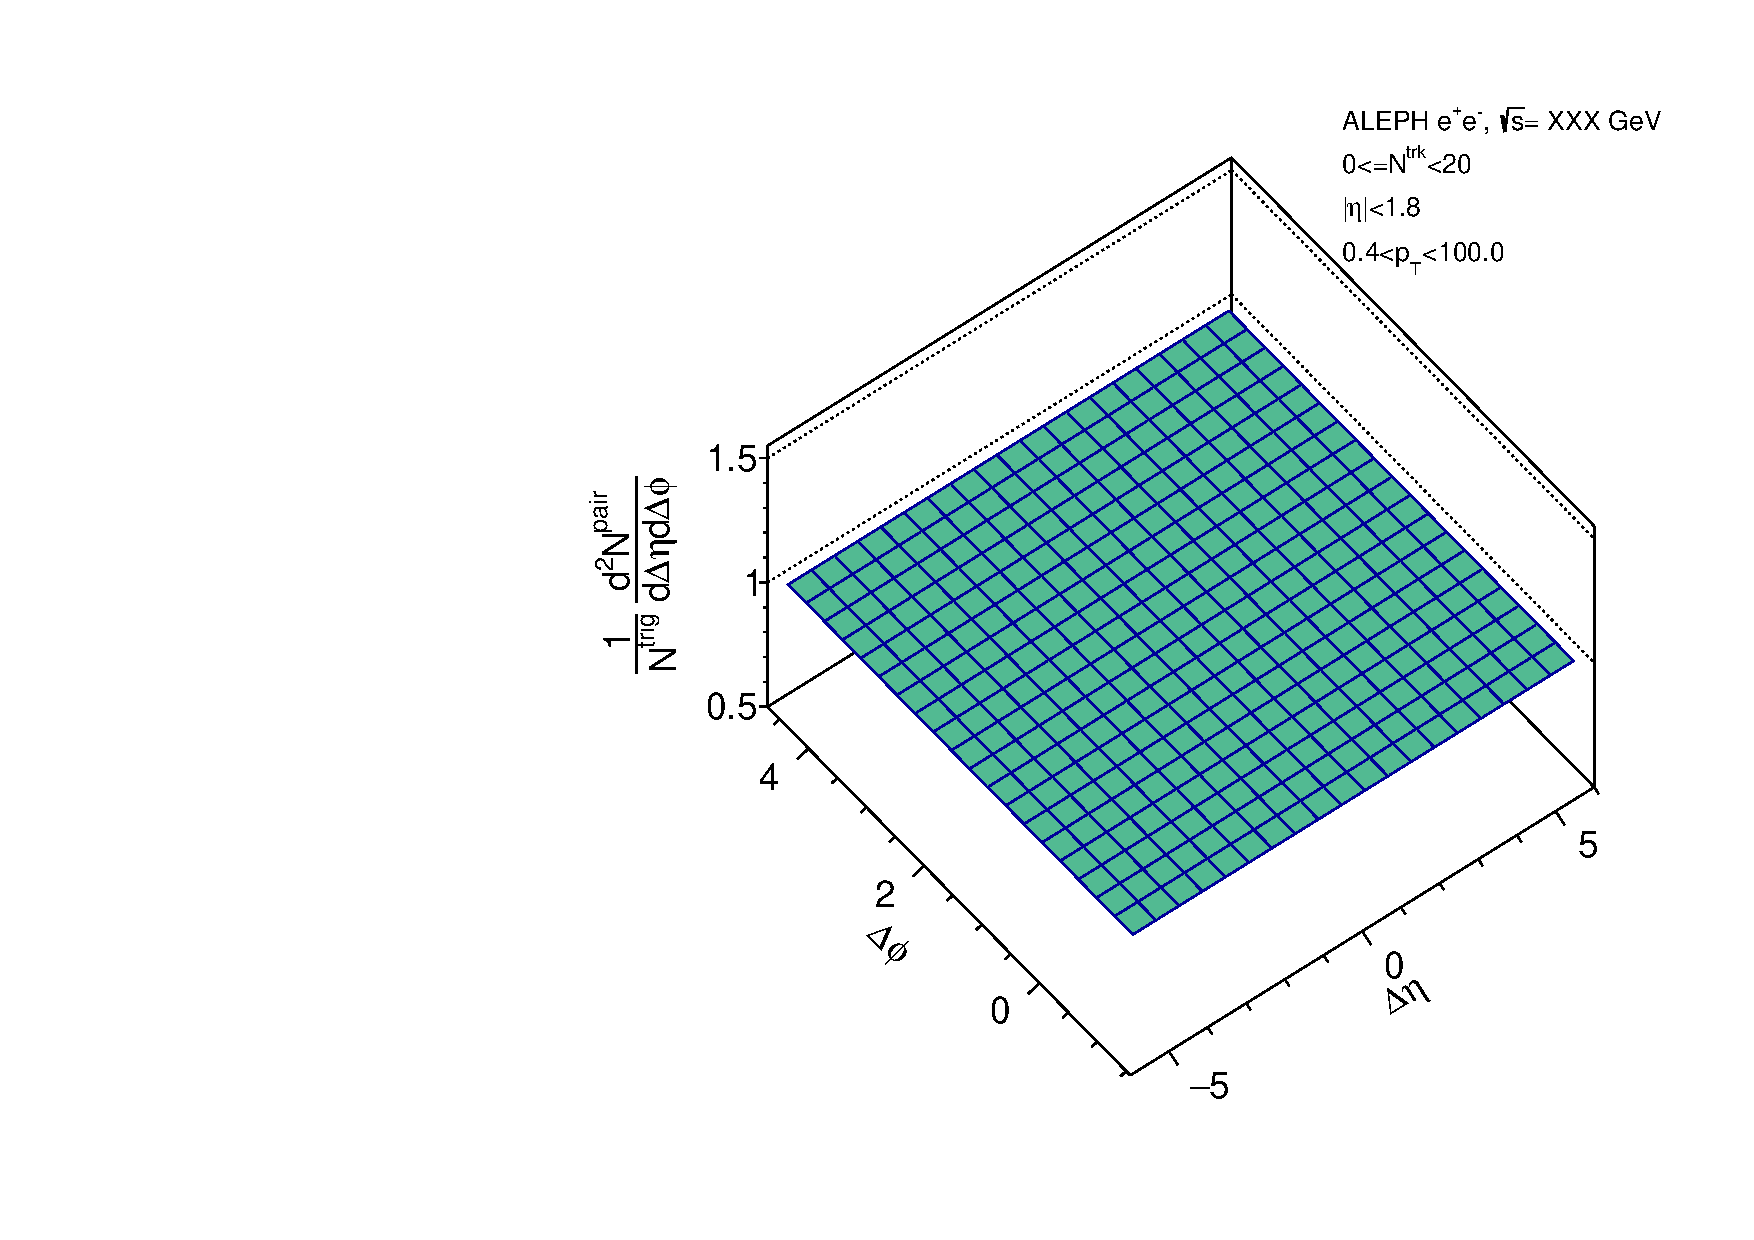
\includegraphics[width=.32\textwidth]{images/TwoParticleCorrelation/CrossCheck/20180126/LEP2_WTA/LEP2_WTA_r_ratio_0_20.pdf}}\hfill
\subfloat{\label{sfig:d}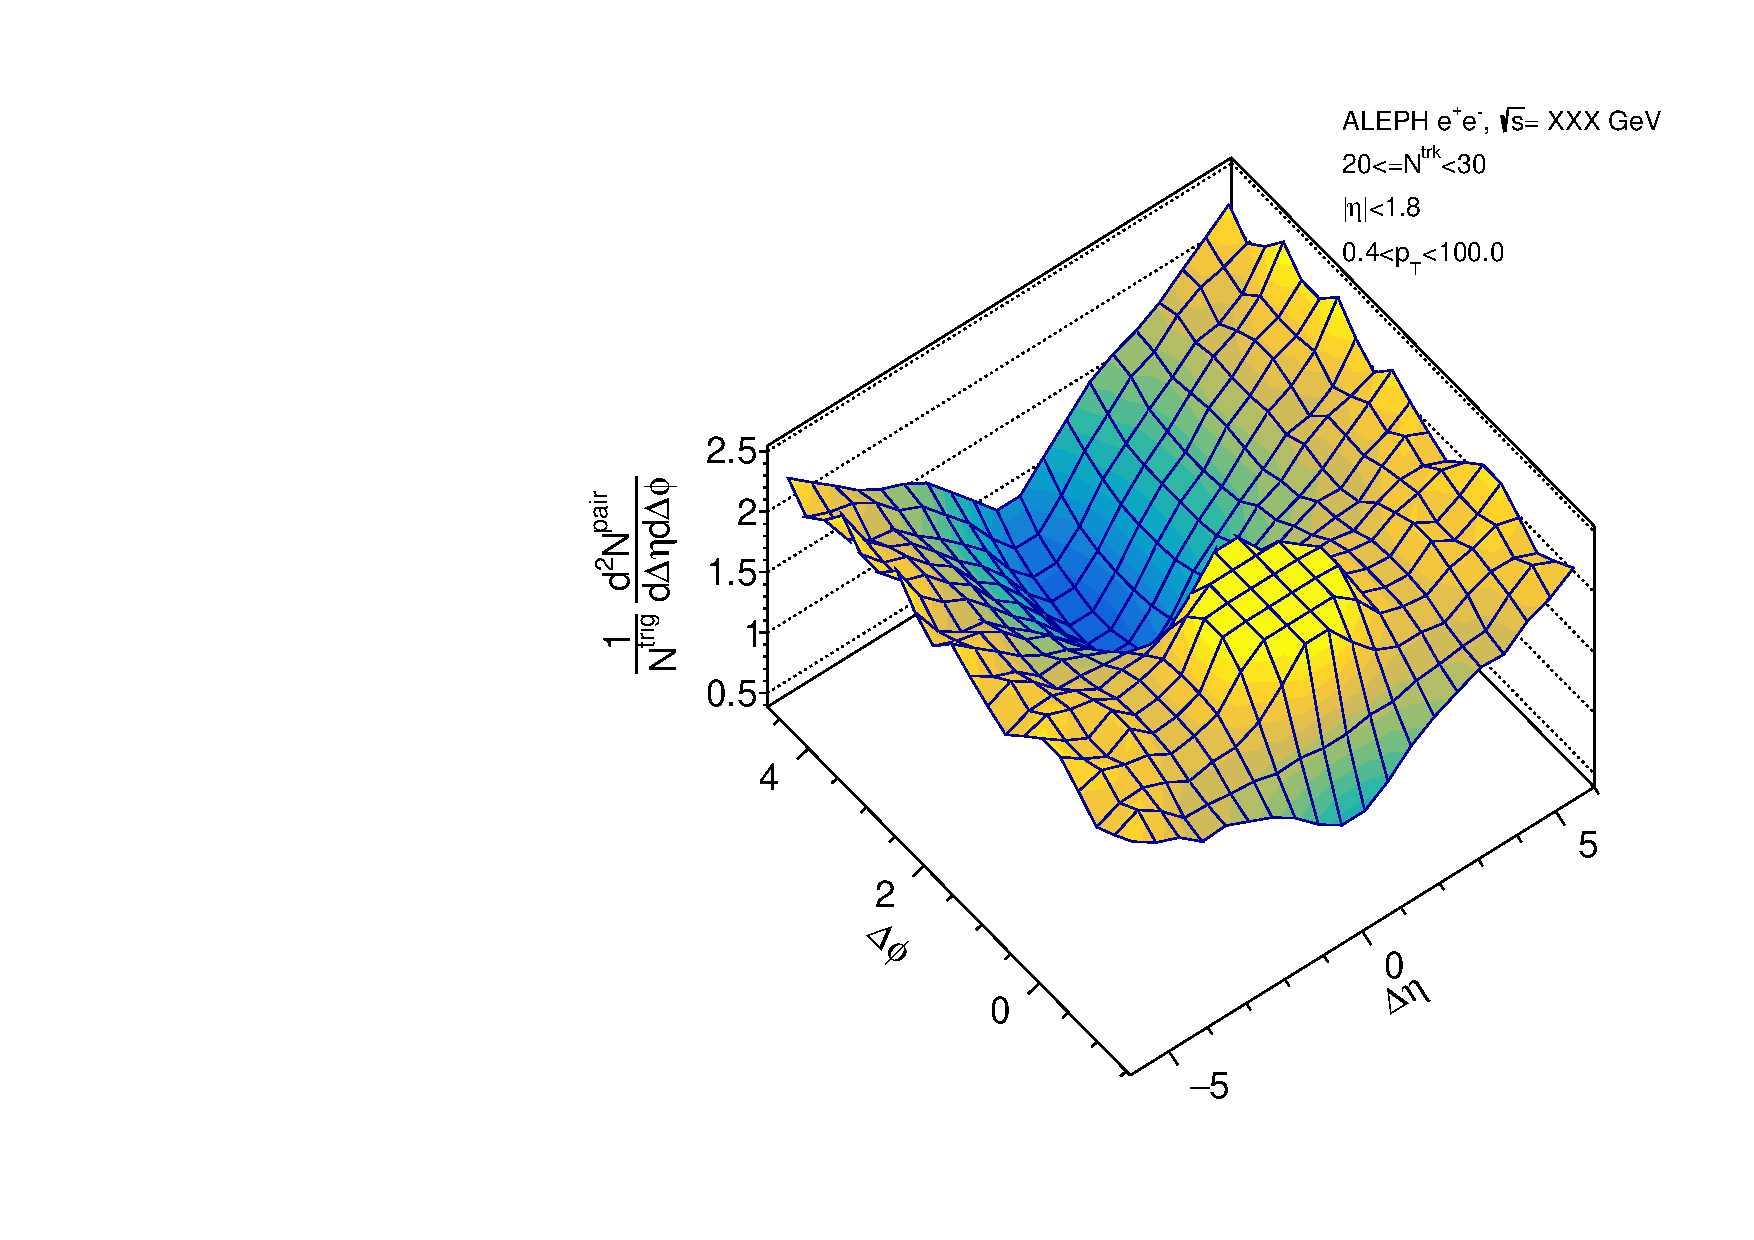
\includegraphics[width=.32\textwidth]{images/TwoParticleCorrelation/CrossCheck/20180126/LEP2_WTA/LEP2_WTA_ratio2_20_30.pdf}}\hfill
\subfloat{\label{sfig:e}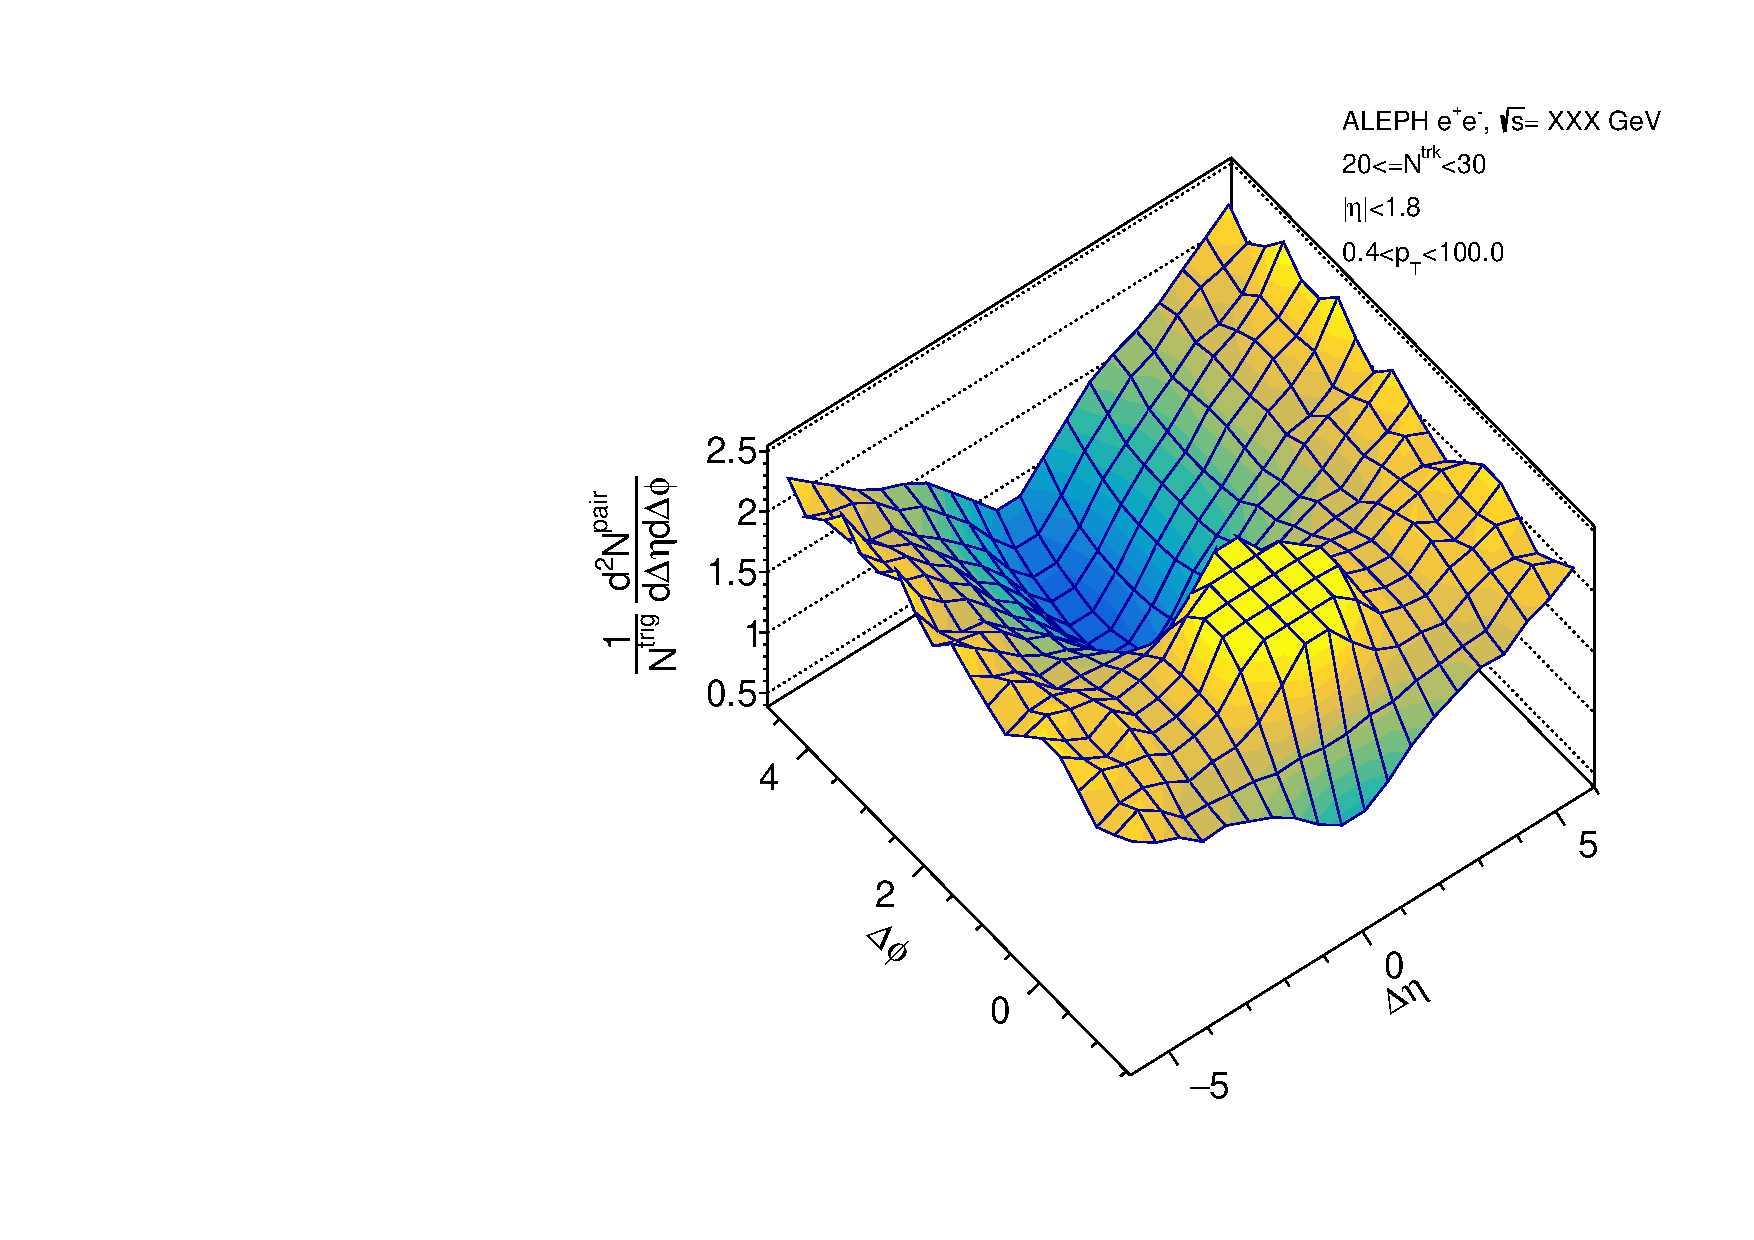
\includegraphics[width=.32\textwidth]{images/TwoParticleCorrelation/CrossCheck/20180126/LEP2_WTA/LEP2_WTA_ratio1_20_30.pdf}}\hfill
\subfloat{\label{sfig:f}\includegraphics[width=.32\textwidth]{images/TwoParticleCorrelation/CrossCheck/20180126/LEP2_WTA/LEP2_WTA_r_ratio_20_30.pdf}}\hfill
\subfloat{\label{sfig:g}\includegraphics[width=.32\textwidth]{images/TwoParticleCorrelation/CrossCheck/20180126/LEP2_WTA/LEP2_WTA_ratio2_30_999.pdf}}\hfill
\subfloat{\label{sfig:h}\includegraphics[width=.32\textwidth]{images/TwoParticleCorrelation/CrossCheck/20180126/LEP2_WTA/LEP2_WTA_ratio1_30_999.pdf}}\hfill
\subfloat{\label{sfig:i}\includegraphics[width=.32\textwidth]{images/TwoParticleCorrelation/CrossCheck/20180126/LEP2_WTA/LEP2_WTA_r_ratio_30_999.pdf}} \\
\caption{Two particle correlation fuctions for the LEP2 data set analyzed in the WTA axis.}
\label{fig:test}
\end{figure}

%%%%%%%%%%% PYTHIA8 %%%%%%%%%%%
\begin{figure}[H]
\centering
\subfloat{\label{sfig:a}\includegraphics[width=.32\textwidth]{images/TwoParticleCorrelation/CrossCheck/20180126/PYTHIA8_WTA/PYTHIA8_WTA_ratio2_0_20.pdf}}\hfill
\subfloat{\label{sfig:b}\includegraphics[width=.32\textwidth]{images/TwoParticleCorrelation/CrossCheck/20180126/PYTHIA8_WTA/PYTHIA8_WTA_ratio1_0_20.pdf}}\hfill
\subfloat{\label{sfig:c}\includegraphics[width=.32\textwidth]{images/TwoParticleCorrelation/CrossCheck/20180126/PYTHIA8_WTA/PYTHIA8_WTA_r_ratio_0_20.pdf}}\hfill
\subfloat{\label{sfig:d}\includegraphics[width=.32\textwidth]{images/TwoParticleCorrelation/CrossCheck/20180126/PYTHIA8_WTA/PYTHIA8_WTA_ratio2_20_30.pdf}}\hfill
\subfloat{\label{sfig:e}\includegraphics[width=.32\textwidth]{images/TwoParticleCorrelation/CrossCheck/20180126/PYTHIA8_WTA/PYTHIA8_WTA_ratio1_20_30.pdf}}\hfill
\subfloat{\label{sfig:f}\includegraphics[width=.32\textwidth]{images/TwoParticleCorrelation/CrossCheck/20180126/PYTHIA8_WTA/PYTHIA8_WTA_r_ratio_20_30.pdf}}\hfill
\subfloat{\label{sfig:g}\includegraphics[width=.32\textwidth]{images/TwoParticleCorrelation/CrossCheck/20180126/PYTHIA8_WTA/PYTHIA8_WTA_ratio2_30_999.pdf}}\hfill
\subfloat{\label{sfig:h}\includegraphics[width=.32\textwidth]{images/TwoParticleCorrelation/CrossCheck/20180126/PYTHIA8_WTA/PYTHIA8_WTA_ratio1_30_999.pdf}}\hfill
\subfloat{\label{sfig:i}\includegraphics[width=.32\textwidth]{images/TwoParticleCorrelation/CrossCheck/20180126/PYTHIA8_WTA/PYTHIA8_WTA_r_ratio_30_999.pdf}} \\
\caption{Two particle correlation fuctions for the PYTHIA8 data set analyzed in the WTA axis.}
\label{fig:test}
\end{figure}


%%%%%%%%%%% PYTHIA8 Rope Walk %%%%%%%%%%%
\begin{figure}[H]
\centering
\subfloat{\label{sfig:a}\includegraphics[width=.32\textwidth]{images/TwoParticleCorrelation/CrossCheck/20180126/PYTHIA8_RopeWalk_WTA/PYTHIA8_RopeWalk_WTA_ratio2_0_20.pdf}}\hfill
\subfloat{\label{sfig:b}\includegraphics[width=.32\textwidth]{images/TwoParticleCorrelation/CrossCheck/20180126/PYTHIA8_RopeWalk_WTA/PYTHIA8_RopeWalk_WTA_ratio1_0_20.pdf}}\hfill
\subfloat{\label{sfig:c}\includegraphics[width=.32\textwidth]{images/TwoParticleCorrelation/CrossCheck/20180126/PYTHIA8_RopeWalk_WTA/PYTHIA8_RopeWalk_WTA_r_ratio_0_20.pdf}}\hfill
\subfloat{\label{sfig:d}\includegraphics[width=.32\textwidth]{images/TwoParticleCorrelation/CrossCheck/20180126/PYTHIA8_RopeWalk_WTA/PYTHIA8_RopeWalk_WTA_ratio2_20_30.pdf}}\hfill
\subfloat{\label{sfig:e}\includegraphics[width=.32\textwidth]{images/TwoParticleCorrelation/CrossCheck/20180126/PYTHIA8_RopeWalk_WTA/PYTHIA8_RopeWalk_WTA_ratio1_20_30.pdf}}\hfill
\subfloat{\label{sfig:f}\includegraphics[width=.32\textwidth]{images/TwoParticleCorrelation/CrossCheck/20180126/PYTHIA8_RopeWalk_WTA/PYTHIA8_RopeWalk_WTA_r_ratio_20_30.pdf}}\hfill
\subfloat{\label{sfig:g}\includegraphics[width=.32\textwidth]{images/TwoParticleCorrelation/CrossCheck/20180126/PYTHIA8_RopeWalk_WTA/PYTHIA8_RopeWalk_WTA_ratio2_30_999.pdf}}\hfill
\subfloat{\label{sfig:h}\includegraphics[width=.32\textwidth]{images/TwoParticleCorrelation/CrossCheck/20180126/PYTHIA8_RopeWalk_WTA/PYTHIA8_RopeWalk_WTA_ratio1_30_999.pdf}}\hfill
\subfloat{\label{sfig:i}\includegraphics[width=.32\textwidth]{images/TwoParticleCorrelation/CrossCheck/20180126/PYTHIA8_RopeWalk_WTA/PYTHIA8_RopeWalk_WTA_r_ratio_30_999.pdf}} \\
\caption{Two particle correlation fuctions for the PYTHIA8 rope walk data set analyzed in the WTA axis.}
\label{fig:test}
\end{figure}
